\documentclass[twoside]{book}

% Packages required by doxygen
\usepackage{fixltx2e}
\usepackage{calc}
\usepackage{doxygen}
\usepackage[export]{adjustbox} % also loads graphicx
\usepackage{graphicx}
\usepackage[utf8]{inputenc}
\usepackage{makeidx}
\usepackage{multicol}
\usepackage{multirow}
\PassOptionsToPackage{warn}{textcomp}
\usepackage{textcomp}
\usepackage[nointegrals]{wasysym}
\usepackage[table]{xcolor}

% NLS support packages
platex
% Font selection
\usepackage[T1]{fontenc}
\usepackage[scaled=.90]{helvet}
\usepackage{courier}
\usepackage{amssymb}
\usepackage{sectsty}
\renewcommand{\familydefault}{\sfdefault}
\allsectionsfont{%
  \fontseries{bc}\selectfont%
  \color{darkgray}%
}
\renewcommand{\DoxyLabelFont}{%
  \fontseries{bc}\selectfont%
  \color{darkgray}%
}
\newcommand{\+}{\discretionary{\mbox{\scriptsize$\hookleftarrow$}}{}{}}

% Page & text layout
\usepackage{geometry}
\geometry{%
  a4paper,%
  top=2.5cm,%
  bottom=2.5cm,%
  left=2.5cm,%
  right=2.5cm%
}
\tolerance=750
\hfuzz=15pt
\hbadness=750
\setlength{\emergencystretch}{15pt}
\setlength{\parindent}{0cm}
\setlength{\parskip}{3ex plus 2ex minus 2ex}
\makeatletter
\renewcommand{\paragraph}{%
  \@startsection{paragraph}{4}{0ex}{-1.0ex}{1.0ex}{%
    \normalfont\normalsize\bfseries\SS@parafont%
  }%
}
\renewcommand{\subparagraph}{%
  \@startsection{subparagraph}{5}{0ex}{-1.0ex}{1.0ex}{%
    \normalfont\normalsize\bfseries\SS@subparafont%
  }%
}
\makeatother

% Headers & footers
\usepackage{fancyhdr}
\pagestyle{fancyplain}
\fancyhead[LE]{\fancyplain{}{\bfseries\thepage}}
\fancyhead[CE]{\fancyplain{}{}}
\fancyhead[RE]{\fancyplain{}{\bfseries\leftmark}}
\fancyhead[LO]{\fancyplain{}{\bfseries\rightmark}}
\fancyhead[CO]{\fancyplain{}{}}
\fancyhead[RO]{\fancyplain{}{\bfseries\thepage}}
\fancyfoot[LE]{\fancyplain{}{}}
\fancyfoot[CE]{\fancyplain{}{}}
\fancyfoot[RE]{\fancyplain{}{\bfseries\scriptsize Generated by Doxygen }}
\fancyfoot[LO]{\fancyplain{}{\bfseries\scriptsize Generated by Doxygen }}
\fancyfoot[CO]{\fancyplain{}{}}
\fancyfoot[RO]{\fancyplain{}{}}
\renewcommand{\footrulewidth}{0.4pt}
\renewcommand{\chaptermark}[1]{%
  \markboth{#1}{}%
}
\renewcommand{\sectionmark}[1]{%
  \markright{\thesection\ #1}%
}

% Indices & bibliography
\usepackage{natbib}
\usepackage[titles]{tocloft}
\setcounter{tocdepth}{3}
\setcounter{secnumdepth}{5}
\makeindex

% Hyperlinks (required, but should be loaded last)
\usepackage{ifpdf}
\ifpdf
  \usepackage[pdftex,pagebackref=true]{hyperref}
\else
  \usepackage[ps2pdf,pagebackref=true]{hyperref}
\fi
\hypersetup{%
  colorlinks=true,%
  linkcolor=blue,%
  citecolor=blue,%
  unicode%
}

% Custom commands
\newcommand{\clearemptydoublepage}{%
  \newpage{\pagestyle{empty}\cleardoublepage}%
}

\usepackage{caption}
\captionsetup{labelsep=space,justification=centering,font={bf},singlelinecheck=off,skip=4pt,position=top}

%===== C O N T E N T S =====

\begin{document}

% Titlepage & ToC
\hypersetup{pageanchor=false,
             bookmarksnumbered=true,
             pdfencoding=unicode
            }
\pagenumbering{alph}
\begin{titlepage}
\vspace*{7cm}
\begin{center}%
{\Large Javaトランプカードプロジェクト \\[1ex]\large 1.\+0.\+0 }\\
\vspace*{1cm}
{\large Generated by Doxygen 1.8.13}\\
\end{center}
\end{titlepage}
\clearemptydoublepage
\pagenumbering{roman}
\tableofcontents
\clearemptydoublepage
\pagenumbering{arabic}
\hypersetup{pageanchor=true}

%--- Begin generated contents ---
\chapter{Class Index}
\section{Class List}
Here are the classes, structs, unions and interfaces with brief descriptions\+:\begin{DoxyCompactList}
\item\contentsline{section}{\hyperlink{classjp_1_1gr_1_1java__conf_1_1yuta__yoshinaga_1_1java__trumpcards_1_1_black_jack}{jp.\+gr.\+java\+\_\+conf.\+yuta\+\_\+yoshinaga.\+java\+\_\+trumpcards.\+Black\+Jack} \\*ブラックジャッククラス }{\pageref{classjp_1_1gr_1_1java__conf_1_1yuta__yoshinaga_1_1java__trumpcards_1_1_black_jack}}{}
\item\contentsline{section}{\hyperlink{classjp_1_1gr_1_1java__conf_1_1yuta__yoshinaga_1_1java__trumpcards_1_1_card}{jp.\+gr.\+java\+\_\+conf.\+yuta\+\_\+yoshinaga.\+java\+\_\+trumpcards.\+Card} \\*カードクラス }{\pageref{classjp_1_1gr_1_1java__conf_1_1yuta__yoshinaga_1_1java__trumpcards_1_1_card}}{}
\item\contentsline{section}{\hyperlink{classjp_1_1gr_1_1java__conf_1_1yuta__yoshinaga_1_1java__trumpcards_1_1_player}{jp.\+gr.\+java\+\_\+conf.\+yuta\+\_\+yoshinaga.\+java\+\_\+trumpcards.\+Player} \\*プレイヤークラス }{\pageref{classjp_1_1gr_1_1java__conf_1_1yuta__yoshinaga_1_1java__trumpcards_1_1_player}}{}
\item\contentsline{section}{\hyperlink{classjp_1_1gr_1_1java__conf_1_1yuta__yoshinaga_1_1java__trumpcards_1_1_trump_cards}{jp.\+gr.\+java\+\_\+conf.\+yuta\+\_\+yoshinaga.\+java\+\_\+trumpcards.\+Trump\+Cards} \\*トランプカードクラス }{\pageref{classjp_1_1gr_1_1java__conf_1_1yuta__yoshinaga_1_1java__trumpcards_1_1_trump_cards}}{}
\end{DoxyCompactList}

\chapter{File Index}
\section{File List}
Here is a list of all documented files with brief descriptions\+:\begin{DoxyCompactList}
\item\contentsline{section}{jp/gr/java\+\_\+conf/yuta\+\_\+yoshinaga/java\+\_\+trumpcards/\hyperlink{_black_jack_8java}{Black\+Jack.\+java} \\*ブラックジャッククラス }{\pageref{_black_jack_8java}}{}
\item\contentsline{section}{jp/gr/java\+\_\+conf/yuta\+\_\+yoshinaga/java\+\_\+trumpcards/\hyperlink{_black_jack_main_8java}{Black\+Jack\+Main.\+java} \\*ブラックジャックメインクラス }{\pageref{_black_jack_main_8java}}{}
\item\contentsline{section}{jp/gr/java\+\_\+conf/yuta\+\_\+yoshinaga/java\+\_\+trumpcards/\hyperlink{_card_8java}{Card.\+java} \\*カードクラス }{\pageref{_card_8java}}{}
\item\contentsline{section}{jp/gr/java\+\_\+conf/yuta\+\_\+yoshinaga/java\+\_\+trumpcards/\hyperlink{_player_8java}{Player.\+java} \\*プレイヤークラス }{\pageref{_player_8java}}{}
\item\contentsline{section}{jp/gr/java\+\_\+conf/yuta\+\_\+yoshinaga/java\+\_\+trumpcards/\hyperlink{_trump_cards_8java}{Trump\+Cards.\+java} \\*トランプカードクラス }{\pageref{_trump_cards_8java}}{}
\end{DoxyCompactList}

\chapter{Class Documentation}
\hypertarget{classjp_1_1gr_1_1java__conf_1_1yuta__yoshinaga_1_1java__trumpcards_1_1_black_jack}{}\section{jp.\+gr.\+java\+\_\+conf.\+yuta\+\_\+yoshinaga.\+java\+\_\+trumpcards.\+Black\+Jack Class Reference}
\label{classjp_1_1gr_1_1java__conf_1_1yuta__yoshinaga_1_1java__trumpcards_1_1_black_jack}\index{jp.\+gr.\+java\+\_\+conf.\+yuta\+\_\+yoshinaga.\+java\+\_\+trumpcards.\+Black\+Jack@{jp.\+gr.\+java\+\_\+conf.\+yuta\+\_\+yoshinaga.\+java\+\_\+trumpcards.\+Black\+Jack}}


ブラックジャッククラス  




Collaboration diagram for jp.\+gr.\+java\+\_\+conf.\+yuta\+\_\+yoshinaga.\+java\+\_\+trumpcards.\+Black\+Jack\+:
\nopagebreak
\begin{figure}[H]
\begin{center}
\leavevmode
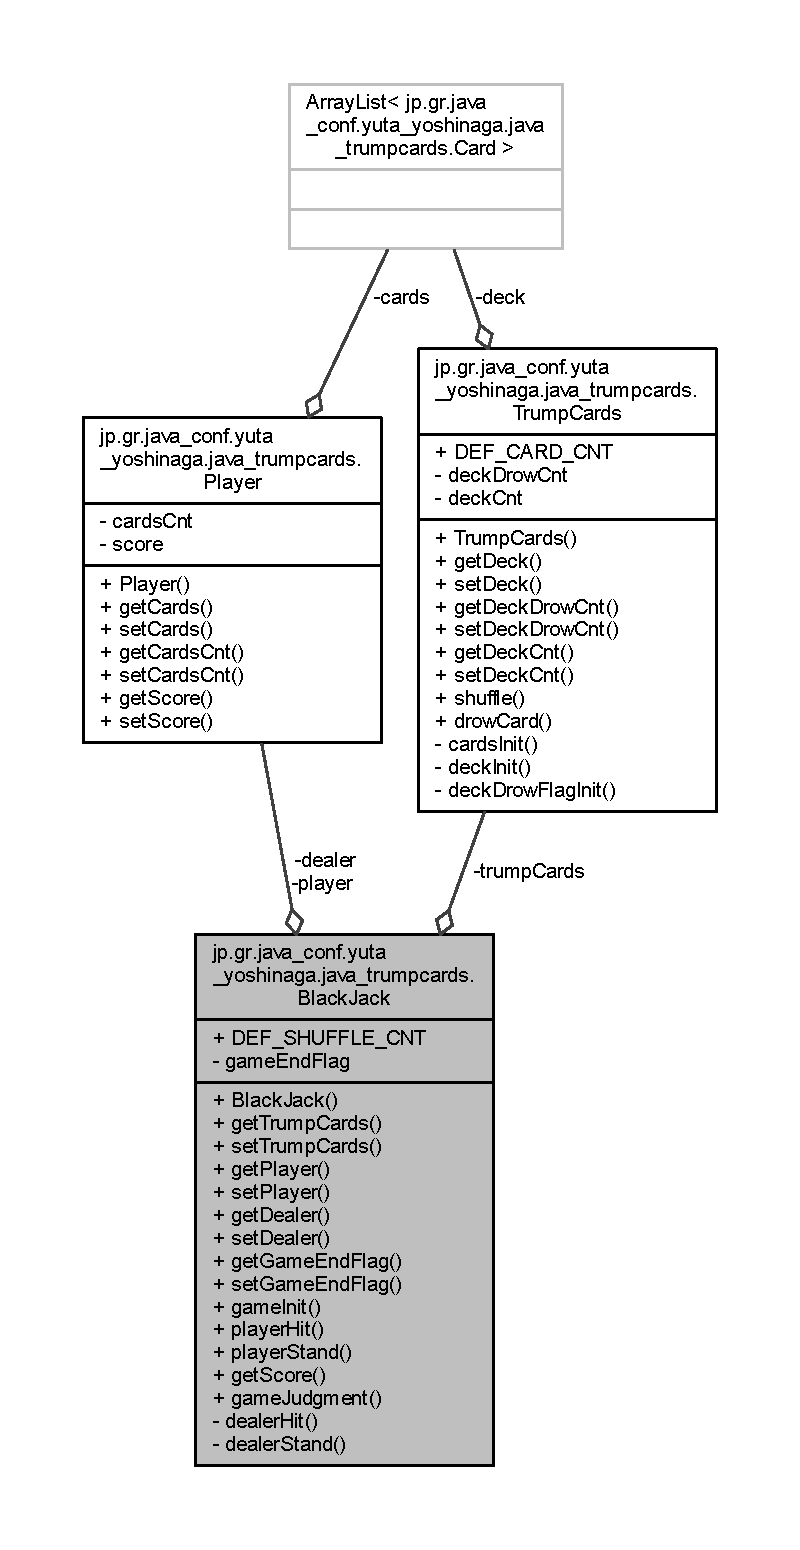
\includegraphics[height=550pt]{classjp_1_1gr_1_1java__conf_1_1yuta__yoshinaga_1_1java__trumpcards_1_1_black_jack__coll__graph}
\end{center}
\end{figure}
\subsection*{Public Member Functions}
\begin{DoxyCompactItemize}
\item 
\hyperlink{classjp_1_1gr_1_1java__conf_1_1yuta__yoshinaga_1_1java__trumpcards_1_1_black_jack_a8ec4c341c5db71243c0916980549868d}{Black\+Jack} ()
\begin{DoxyCompactList}\small\item\em コンストラクタ \end{DoxyCompactList}\item 
\hyperlink{classjp_1_1gr_1_1java__conf_1_1yuta__yoshinaga_1_1java__trumpcards_1_1_trump_cards}{Trump\+Cards} \hyperlink{classjp_1_1gr_1_1java__conf_1_1yuta__yoshinaga_1_1java__trumpcards_1_1_black_jack_a19f0d24ac49d16b9db099801cc6f7340}{get\+Trump\+Cards} ()
\begin{DoxyCompactList}\small\item\em ゲッター \end{DoxyCompactList}\item 
void \hyperlink{classjp_1_1gr_1_1java__conf_1_1yuta__yoshinaga_1_1java__trumpcards_1_1_black_jack_a216185ef3f8c02439b201ec52234aecf}{set\+Trump\+Cards} (\hyperlink{classjp_1_1gr_1_1java__conf_1_1yuta__yoshinaga_1_1java__trumpcards_1_1_trump_cards}{Trump\+Cards} \hyperlink{classjp_1_1gr_1_1java__conf_1_1yuta__yoshinaga_1_1java__trumpcards_1_1_black_jack_a7961e6ab54f14237d136f6be831f3014}{trump\+Cards})
\begin{DoxyCompactList}\small\item\em セッター \end{DoxyCompactList}\item 
\hyperlink{classjp_1_1gr_1_1java__conf_1_1yuta__yoshinaga_1_1java__trumpcards_1_1_player}{Player} \hyperlink{classjp_1_1gr_1_1java__conf_1_1yuta__yoshinaga_1_1java__trumpcards_1_1_black_jack_aa4fff12d377006ce93d731a6808b67bd}{get\+Player} ()
\begin{DoxyCompactList}\small\item\em ゲッター \end{DoxyCompactList}\item 
void \hyperlink{classjp_1_1gr_1_1java__conf_1_1yuta__yoshinaga_1_1java__trumpcards_1_1_black_jack_a3c6bfcfb81ccad65be2f5cfb82819951}{set\+Player} (\hyperlink{classjp_1_1gr_1_1java__conf_1_1yuta__yoshinaga_1_1java__trumpcards_1_1_player}{Player} \hyperlink{classjp_1_1gr_1_1java__conf_1_1yuta__yoshinaga_1_1java__trumpcards_1_1_black_jack_a94a3eaa560ab93f938ce2c26dad52eb4}{player})
\begin{DoxyCompactList}\small\item\em セッター \end{DoxyCompactList}\item 
\hyperlink{classjp_1_1gr_1_1java__conf_1_1yuta__yoshinaga_1_1java__trumpcards_1_1_player}{Player} \hyperlink{classjp_1_1gr_1_1java__conf_1_1yuta__yoshinaga_1_1java__trumpcards_1_1_black_jack_ae3829512336f2ca3f931924b435c8593}{get\+Dealer} ()
\begin{DoxyCompactList}\small\item\em ゲッター \end{DoxyCompactList}\item 
void \hyperlink{classjp_1_1gr_1_1java__conf_1_1yuta__yoshinaga_1_1java__trumpcards_1_1_black_jack_a8fd066f80b7dd83f393a770bb24cd675}{set\+Dealer} (\hyperlink{classjp_1_1gr_1_1java__conf_1_1yuta__yoshinaga_1_1java__trumpcards_1_1_player}{Player} \hyperlink{classjp_1_1gr_1_1java__conf_1_1yuta__yoshinaga_1_1java__trumpcards_1_1_black_jack_a01acee20012cd234246a1b058cc9d8c0}{dealer})
\begin{DoxyCompactList}\small\item\em セッター \end{DoxyCompactList}\item 
boolean \hyperlink{classjp_1_1gr_1_1java__conf_1_1yuta__yoshinaga_1_1java__trumpcards_1_1_black_jack_aa541fa5982861610f084bede8c5d6ac1}{get\+Game\+End\+Flag} ()
\begin{DoxyCompactList}\small\item\em ゲッター \end{DoxyCompactList}\item 
void \hyperlink{classjp_1_1gr_1_1java__conf_1_1yuta__yoshinaga_1_1java__trumpcards_1_1_black_jack_a75ef56d0490e7b343fc6c02acbe43dd7}{set\+Game\+End\+Flag} (boolean \hyperlink{classjp_1_1gr_1_1java__conf_1_1yuta__yoshinaga_1_1java__trumpcards_1_1_black_jack_a91aefa2a1168d70726ddb68735bfe9fe}{game\+End\+Flag})
\begin{DoxyCompactList}\small\item\em セッター \end{DoxyCompactList}\item 
void \hyperlink{classjp_1_1gr_1_1java__conf_1_1yuta__yoshinaga_1_1java__trumpcards_1_1_black_jack_aecf1c840d9643b4809cd5e93710256a4}{game\+Init} ()
\begin{DoxyCompactList}\small\item\em ゲーム初期化 \end{DoxyCompactList}\item 
void \hyperlink{classjp_1_1gr_1_1java__conf_1_1yuta__yoshinaga_1_1java__trumpcards_1_1_black_jack_a4b8f2248ac868b5d3b9506fb0ece0ea2}{player\+Hit} ()
\begin{DoxyCompactList}\small\item\em プレイヤーヒット \end{DoxyCompactList}\item 
void \hyperlink{classjp_1_1gr_1_1java__conf_1_1yuta__yoshinaga_1_1java__trumpcards_1_1_black_jack_a53f37ae6f1388143c70a8b138c6c2443}{player\+Stand} ()
\begin{DoxyCompactList}\small\item\em プレイヤースタンド \end{DoxyCompactList}\item 
int \hyperlink{classjp_1_1gr_1_1java__conf_1_1yuta__yoshinaga_1_1java__trumpcards_1_1_black_jack_a23b680e89ca3a4c306576ba0a7debfac}{get\+Score} (Array\+List$<$ \hyperlink{classjp_1_1gr_1_1java__conf_1_1yuta__yoshinaga_1_1java__trumpcards_1_1_card}{Card} $>$ cards, int cards\+Cnt)
\begin{DoxyCompactList}\small\item\em 手札から現在のスコア取得 \end{DoxyCompactList}\item 
int \hyperlink{classjp_1_1gr_1_1java__conf_1_1yuta__yoshinaga_1_1java__trumpcards_1_1_black_jack_a26f4a11e36c237ec64f08010b8ea0a01}{game\+Judgment} ()
\begin{DoxyCompactList}\small\item\em ゲーム勝敗判定 \end{DoxyCompactList}\end{DoxyCompactItemize}
\subsection*{Static Public Attributes}
\begin{DoxyCompactItemize}
\item 
\mbox{\Hypertarget{classjp_1_1gr_1_1java__conf_1_1yuta__yoshinaga_1_1java__trumpcards_1_1_black_jack_a6726d858249cdc023cd6e347593b337b}\label{classjp_1_1gr_1_1java__conf_1_1yuta__yoshinaga_1_1java__trumpcards_1_1_black_jack_a6726d858249cdc023cd6e347593b337b}} 
static final int {\bfseries D\+E\+F\+\_\+\+S\+H\+U\+F\+F\+L\+E\+\_\+\+C\+NT} = 10
\end{DoxyCompactItemize}
\subsection*{Private Member Functions}
\begin{DoxyCompactItemize}
\item 
void \hyperlink{classjp_1_1gr_1_1java__conf_1_1yuta__yoshinaga_1_1java__trumpcards_1_1_black_jack_a3db7b3231ab583af54941a41517954ea}{dealer\+Hit} ()
\begin{DoxyCompactList}\small\item\em ディーラーヒット \end{DoxyCompactList}\item 
void \hyperlink{classjp_1_1gr_1_1java__conf_1_1yuta__yoshinaga_1_1java__trumpcards_1_1_black_jack_a49f2f12998ffa9892f4e8212f85afc7f}{dealer\+Stand} ()
\begin{DoxyCompactList}\small\item\em ディーラースタンド \end{DoxyCompactList}\end{DoxyCompactItemize}
\subsection*{Private Attributes}
\begin{DoxyCompactItemize}
\item 
\mbox{\Hypertarget{classjp_1_1gr_1_1java__conf_1_1yuta__yoshinaga_1_1java__trumpcards_1_1_black_jack_a7961e6ab54f14237d136f6be831f3014}\label{classjp_1_1gr_1_1java__conf_1_1yuta__yoshinaga_1_1java__trumpcards_1_1_black_jack_a7961e6ab54f14237d136f6be831f3014}} 
\hyperlink{classjp_1_1gr_1_1java__conf_1_1yuta__yoshinaga_1_1java__trumpcards_1_1_trump_cards}{Trump\+Cards} \hyperlink{classjp_1_1gr_1_1java__conf_1_1yuta__yoshinaga_1_1java__trumpcards_1_1_black_jack_a7961e6ab54f14237d136f6be831f3014}{trump\+Cards}
\begin{DoxyCompactList}\small\item\em トランプカード \end{DoxyCompactList}\item 
\mbox{\Hypertarget{classjp_1_1gr_1_1java__conf_1_1yuta__yoshinaga_1_1java__trumpcards_1_1_black_jack_a94a3eaa560ab93f938ce2c26dad52eb4}\label{classjp_1_1gr_1_1java__conf_1_1yuta__yoshinaga_1_1java__trumpcards_1_1_black_jack_a94a3eaa560ab93f938ce2c26dad52eb4}} 
\hyperlink{classjp_1_1gr_1_1java__conf_1_1yuta__yoshinaga_1_1java__trumpcards_1_1_player}{Player} \hyperlink{classjp_1_1gr_1_1java__conf_1_1yuta__yoshinaga_1_1java__trumpcards_1_1_black_jack_a94a3eaa560ab93f938ce2c26dad52eb4}{player}
\begin{DoxyCompactList}\small\item\em プレイヤー \end{DoxyCompactList}\item 
\mbox{\Hypertarget{classjp_1_1gr_1_1java__conf_1_1yuta__yoshinaga_1_1java__trumpcards_1_1_black_jack_a01acee20012cd234246a1b058cc9d8c0}\label{classjp_1_1gr_1_1java__conf_1_1yuta__yoshinaga_1_1java__trumpcards_1_1_black_jack_a01acee20012cd234246a1b058cc9d8c0}} 
\hyperlink{classjp_1_1gr_1_1java__conf_1_1yuta__yoshinaga_1_1java__trumpcards_1_1_player}{Player} \hyperlink{classjp_1_1gr_1_1java__conf_1_1yuta__yoshinaga_1_1java__trumpcards_1_1_black_jack_a01acee20012cd234246a1b058cc9d8c0}{dealer}
\begin{DoxyCompactList}\small\item\em ディーラー \end{DoxyCompactList}\item 
\mbox{\Hypertarget{classjp_1_1gr_1_1java__conf_1_1yuta__yoshinaga_1_1java__trumpcards_1_1_black_jack_a91aefa2a1168d70726ddb68735bfe9fe}\label{classjp_1_1gr_1_1java__conf_1_1yuta__yoshinaga_1_1java__trumpcards_1_1_black_jack_a91aefa2a1168d70726ddb68735bfe9fe}} 
boolean \hyperlink{classjp_1_1gr_1_1java__conf_1_1yuta__yoshinaga_1_1java__trumpcards_1_1_black_jack_a91aefa2a1168d70726ddb68735bfe9fe}{game\+End\+Flag}
\begin{DoxyCompactList}\small\item\em ゲーム終了フラグ \end{DoxyCompactList}\end{DoxyCompactItemize}


\subsection{Detailed Description}
ブラックジャッククラス 

Definition at line 26 of file Black\+Jack.\+java.



\subsection{Constructor \& Destructor Documentation}
\mbox{\Hypertarget{classjp_1_1gr_1_1java__conf_1_1yuta__yoshinaga_1_1java__trumpcards_1_1_black_jack_a8ec4c341c5db71243c0916980549868d}\label{classjp_1_1gr_1_1java__conf_1_1yuta__yoshinaga_1_1java__trumpcards_1_1_black_jack_a8ec4c341c5db71243c0916980549868d}} 
\index{jp\+::gr\+::java\+\_\+conf\+::yuta\+\_\+yoshinaga\+::java\+\_\+trumpcards\+::\+Black\+Jack@{jp\+::gr\+::java\+\_\+conf\+::yuta\+\_\+yoshinaga\+::java\+\_\+trumpcards\+::\+Black\+Jack}!Black\+Jack@{Black\+Jack}}
\index{Black\+Jack@{Black\+Jack}!jp\+::gr\+::java\+\_\+conf\+::yuta\+\_\+yoshinaga\+::java\+\_\+trumpcards\+::\+Black\+Jack@{jp\+::gr\+::java\+\_\+conf\+::yuta\+\_\+yoshinaga\+::java\+\_\+trumpcards\+::\+Black\+Jack}}
\subsubsection{\texorpdfstring{Black\+Jack()}{BlackJack()}}
{\footnotesize\ttfamily public jp.\+gr.\+java\+\_\+conf.\+yuta\+\_\+yoshinaga.\+java\+\_\+trumpcards.\+Black\+Jack.\+Black\+Jack (\begin{DoxyParamCaption}{ }\end{DoxyParamCaption})}



コンストラクタ 

\begin{DoxyReturn}{Returns}
ありません 
\end{DoxyReturn}
\begin{DoxyAuthor}{Author}
Yuta Yoshinaga 
\end{DoxyAuthor}
\begin{DoxyDate}{Date}
2019.\+04.\+27 
\end{DoxyDate}


Definition at line 41 of file Black\+Jack.\+java.

Here is the call graph for this function\+:
\nopagebreak
\begin{figure}[H]
\begin{center}
\leavevmode
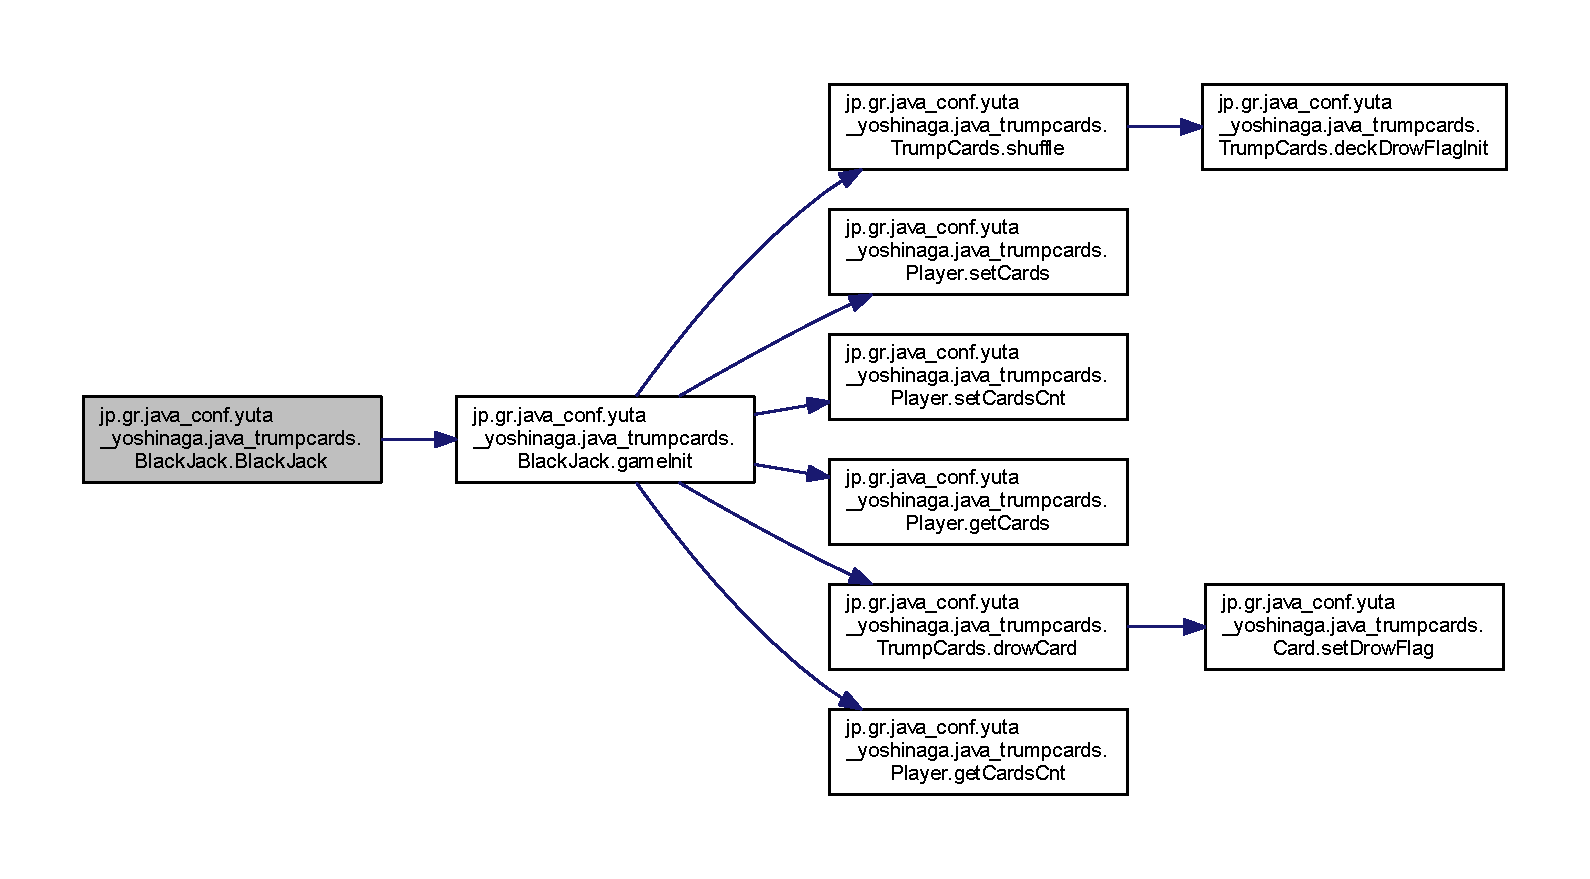
\includegraphics[width=350pt]{classjp_1_1gr_1_1java__conf_1_1yuta__yoshinaga_1_1java__trumpcards_1_1_black_jack_a8ec4c341c5db71243c0916980549868d_cgraph}
\end{center}
\end{figure}


\subsection{Member Function Documentation}
\mbox{\Hypertarget{classjp_1_1gr_1_1java__conf_1_1yuta__yoshinaga_1_1java__trumpcards_1_1_black_jack_a3db7b3231ab583af54941a41517954ea}\label{classjp_1_1gr_1_1java__conf_1_1yuta__yoshinaga_1_1java__trumpcards_1_1_black_jack_a3db7b3231ab583af54941a41517954ea}} 
\index{jp\+::gr\+::java\+\_\+conf\+::yuta\+\_\+yoshinaga\+::java\+\_\+trumpcards\+::\+Black\+Jack@{jp\+::gr\+::java\+\_\+conf\+::yuta\+\_\+yoshinaga\+::java\+\_\+trumpcards\+::\+Black\+Jack}!dealer\+Hit@{dealer\+Hit}}
\index{dealer\+Hit@{dealer\+Hit}!jp\+::gr\+::java\+\_\+conf\+::yuta\+\_\+yoshinaga\+::java\+\_\+trumpcards\+::\+Black\+Jack@{jp\+::gr\+::java\+\_\+conf\+::yuta\+\_\+yoshinaga\+::java\+\_\+trumpcards\+::\+Black\+Jack}}
\subsubsection{\texorpdfstring{dealer\+Hit()}{dealerHit()}}
{\footnotesize\ttfamily private void jp.\+gr.\+java\+\_\+conf.\+yuta\+\_\+yoshinaga.\+java\+\_\+trumpcards.\+Black\+Jack.\+dealer\+Hit (\begin{DoxyParamCaption}{ }\end{DoxyParamCaption})\hspace{0.3cm}{\ttfamily [private]}}



ディーラーヒット 

\begin{DoxyReturn}{Returns}
ありません 
\end{DoxyReturn}
\begin{DoxyAuthor}{Author}
Yuta Yoshinaga 
\end{DoxyAuthor}
\begin{DoxyDate}{Date}
2019.\+04.\+27 
\end{DoxyDate}


Definition at line 214 of file Black\+Jack.\+java.



Referenced by jp.\+gr.\+java\+\_\+conf.\+yuta\+\_\+yoshinaga.\+java\+\_\+trumpcards.\+Black\+Jack.\+player\+Stand().

Here is the call graph for this function\+:
\nopagebreak
\begin{figure}[H]
\begin{center}
\leavevmode
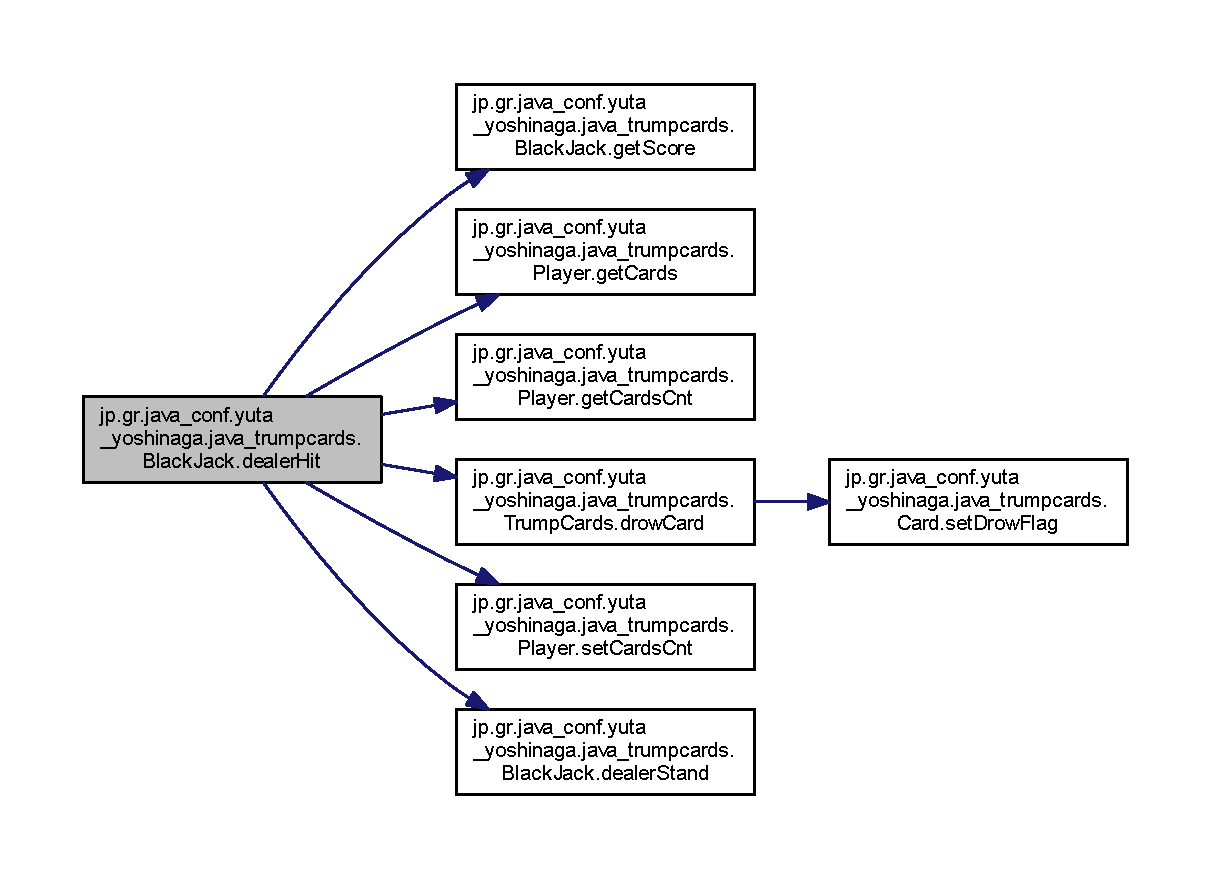
\includegraphics[width=350pt]{classjp_1_1gr_1_1java__conf_1_1yuta__yoshinaga_1_1java__trumpcards_1_1_black_jack_a3db7b3231ab583af54941a41517954ea_cgraph}
\end{center}
\end{figure}
Here is the caller graph for this function\+:
\nopagebreak
\begin{figure}[H]
\begin{center}
\leavevmode
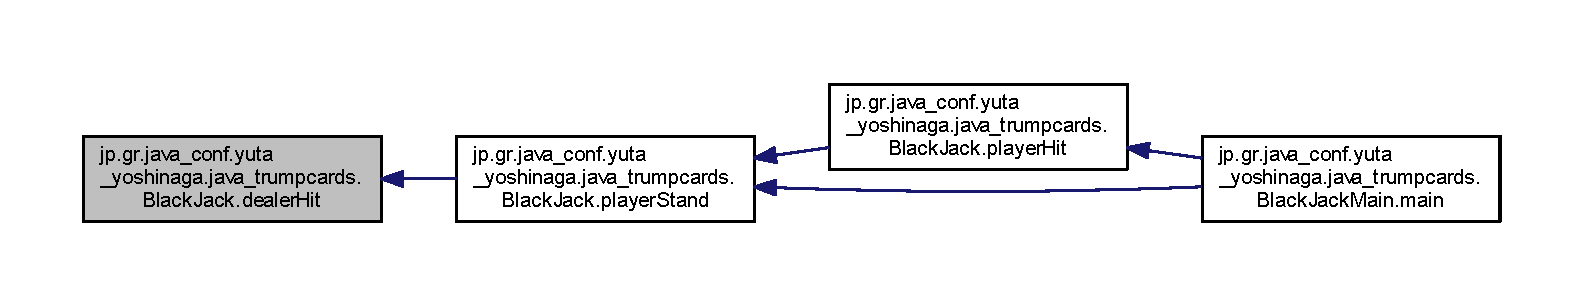
\includegraphics[width=350pt]{classjp_1_1gr_1_1java__conf_1_1yuta__yoshinaga_1_1java__trumpcards_1_1_black_jack_a3db7b3231ab583af54941a41517954ea_icgraph}
\end{center}
\end{figure}
\mbox{\Hypertarget{classjp_1_1gr_1_1java__conf_1_1yuta__yoshinaga_1_1java__trumpcards_1_1_black_jack_a49f2f12998ffa9892f4e8212f85afc7f}\label{classjp_1_1gr_1_1java__conf_1_1yuta__yoshinaga_1_1java__trumpcards_1_1_black_jack_a49f2f12998ffa9892f4e8212f85afc7f}} 
\index{jp\+::gr\+::java\+\_\+conf\+::yuta\+\_\+yoshinaga\+::java\+\_\+trumpcards\+::\+Black\+Jack@{jp\+::gr\+::java\+\_\+conf\+::yuta\+\_\+yoshinaga\+::java\+\_\+trumpcards\+::\+Black\+Jack}!dealer\+Stand@{dealer\+Stand}}
\index{dealer\+Stand@{dealer\+Stand}!jp\+::gr\+::java\+\_\+conf\+::yuta\+\_\+yoshinaga\+::java\+\_\+trumpcards\+::\+Black\+Jack@{jp\+::gr\+::java\+\_\+conf\+::yuta\+\_\+yoshinaga\+::java\+\_\+trumpcards\+::\+Black\+Jack}}
\subsubsection{\texorpdfstring{dealer\+Stand()}{dealerStand()}}
{\footnotesize\ttfamily private void jp.\+gr.\+java\+\_\+conf.\+yuta\+\_\+yoshinaga.\+java\+\_\+trumpcards.\+Black\+Jack.\+dealer\+Stand (\begin{DoxyParamCaption}{ }\end{DoxyParamCaption})\hspace{0.3cm}{\ttfamily [private]}}



ディーラースタンド 

\begin{DoxyReturn}{Returns}
ありません 
\end{DoxyReturn}
\begin{DoxyAuthor}{Author}
Yuta Yoshinaga 
\end{DoxyAuthor}
\begin{DoxyDate}{Date}
2019.\+04.\+27 
\end{DoxyDate}


Definition at line 239 of file Black\+Jack.\+java.



Referenced by jp.\+gr.\+java\+\_\+conf.\+yuta\+\_\+yoshinaga.\+java\+\_\+trumpcards.\+Black\+Jack.\+dealer\+Hit().

Here is the caller graph for this function\+:
\nopagebreak
\begin{figure}[H]
\begin{center}
\leavevmode
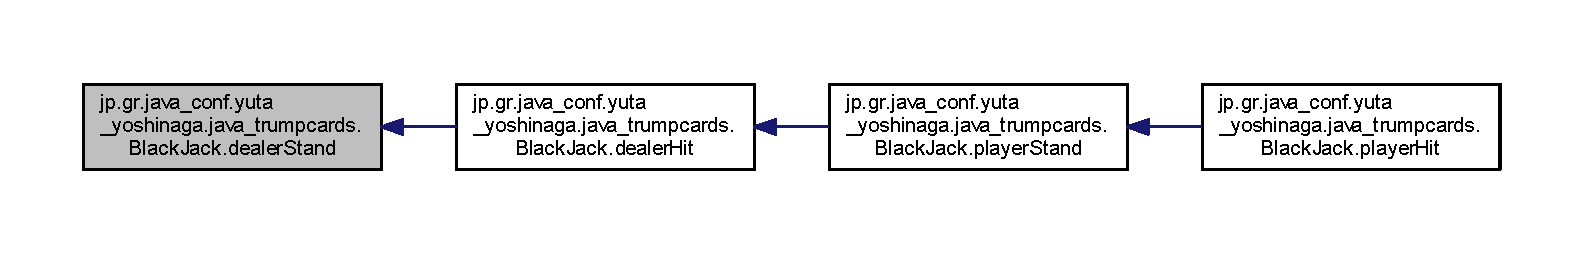
\includegraphics[width=350pt]{classjp_1_1gr_1_1java__conf_1_1yuta__yoshinaga_1_1java__trumpcards_1_1_black_jack_a49f2f12998ffa9892f4e8212f85afc7f_icgraph}
\end{center}
\end{figure}
\mbox{\Hypertarget{classjp_1_1gr_1_1java__conf_1_1yuta__yoshinaga_1_1java__trumpcards_1_1_black_jack_aecf1c840d9643b4809cd5e93710256a4}\label{classjp_1_1gr_1_1java__conf_1_1yuta__yoshinaga_1_1java__trumpcards_1_1_black_jack_aecf1c840d9643b4809cd5e93710256a4}} 
\index{jp\+::gr\+::java\+\_\+conf\+::yuta\+\_\+yoshinaga\+::java\+\_\+trumpcards\+::\+Black\+Jack@{jp\+::gr\+::java\+\_\+conf\+::yuta\+\_\+yoshinaga\+::java\+\_\+trumpcards\+::\+Black\+Jack}!game\+Init@{game\+Init}}
\index{game\+Init@{game\+Init}!jp\+::gr\+::java\+\_\+conf\+::yuta\+\_\+yoshinaga\+::java\+\_\+trumpcards\+::\+Black\+Jack@{jp\+::gr\+::java\+\_\+conf\+::yuta\+\_\+yoshinaga\+::java\+\_\+trumpcards\+::\+Black\+Jack}}
\subsubsection{\texorpdfstring{game\+Init()}{gameInit()}}
{\footnotesize\ttfamily public void jp.\+gr.\+java\+\_\+conf.\+yuta\+\_\+yoshinaga.\+java\+\_\+trumpcards.\+Black\+Jack.\+game\+Init (\begin{DoxyParamCaption}{ }\end{DoxyParamCaption})}



ゲーム初期化 

\begin{DoxyReturn}{Returns}
ありません 
\end{DoxyReturn}
\begin{DoxyAuthor}{Author}
Yuta Yoshinaga 
\end{DoxyAuthor}
\begin{DoxyDate}{Date}
2019.\+04.\+27 
\end{DoxyDate}


Definition at line 156 of file Black\+Jack.\+java.



Referenced by jp.\+gr.\+java\+\_\+conf.\+yuta\+\_\+yoshinaga.\+java\+\_\+trumpcards.\+Black\+Jack.\+Black\+Jack().

Here is the call graph for this function\+:
\nopagebreak
\begin{figure}[H]
\begin{center}
\leavevmode
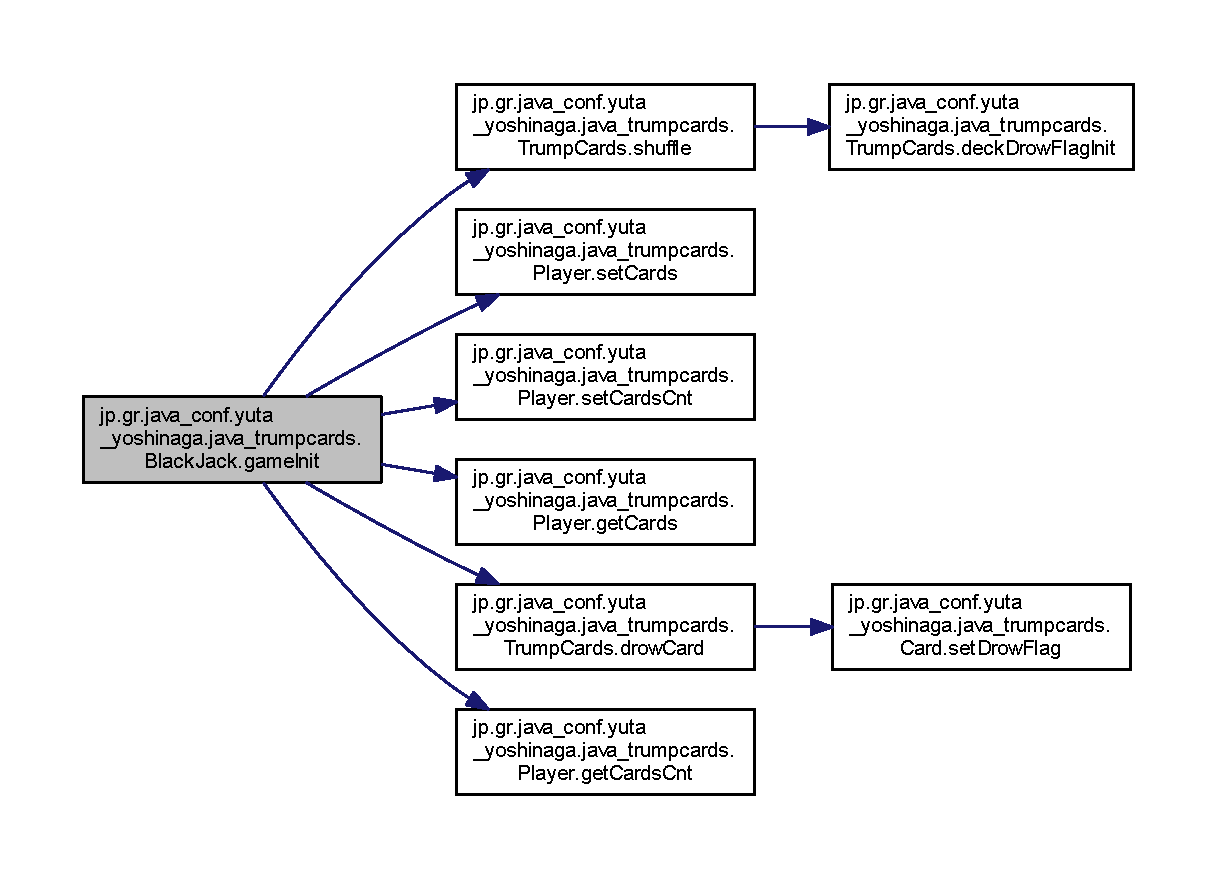
\includegraphics[width=350pt]{classjp_1_1gr_1_1java__conf_1_1yuta__yoshinaga_1_1java__trumpcards_1_1_black_jack_aecf1c840d9643b4809cd5e93710256a4_cgraph}
\end{center}
\end{figure}
Here is the caller graph for this function\+:
\nopagebreak
\begin{figure}[H]
\begin{center}
\leavevmode
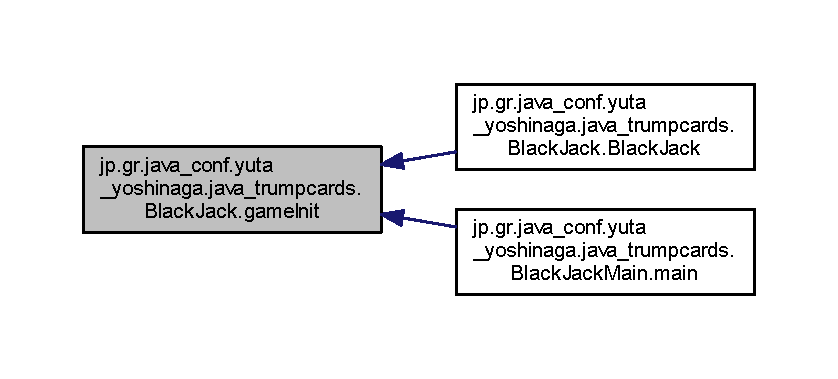
\includegraphics[width=350pt]{classjp_1_1gr_1_1java__conf_1_1yuta__yoshinaga_1_1java__trumpcards_1_1_black_jack_aecf1c840d9643b4809cd5e93710256a4_icgraph}
\end{center}
\end{figure}
\mbox{\Hypertarget{classjp_1_1gr_1_1java__conf_1_1yuta__yoshinaga_1_1java__trumpcards_1_1_black_jack_a26f4a11e36c237ec64f08010b8ea0a01}\label{classjp_1_1gr_1_1java__conf_1_1yuta__yoshinaga_1_1java__trumpcards_1_1_black_jack_a26f4a11e36c237ec64f08010b8ea0a01}} 
\index{jp\+::gr\+::java\+\_\+conf\+::yuta\+\_\+yoshinaga\+::java\+\_\+trumpcards\+::\+Black\+Jack@{jp\+::gr\+::java\+\_\+conf\+::yuta\+\_\+yoshinaga\+::java\+\_\+trumpcards\+::\+Black\+Jack}!game\+Judgment@{game\+Judgment}}
\index{game\+Judgment@{game\+Judgment}!jp\+::gr\+::java\+\_\+conf\+::yuta\+\_\+yoshinaga\+::java\+\_\+trumpcards\+::\+Black\+Jack@{jp\+::gr\+::java\+\_\+conf\+::yuta\+\_\+yoshinaga\+::java\+\_\+trumpcards\+::\+Black\+Jack}}
\subsubsection{\texorpdfstring{game\+Judgment()}{gameJudgment()}}
{\footnotesize\ttfamily public int jp.\+gr.\+java\+\_\+conf.\+yuta\+\_\+yoshinaga.\+java\+\_\+trumpcards.\+Black\+Jack.\+game\+Judgment (\begin{DoxyParamCaption}{ }\end{DoxyParamCaption})}



ゲーム勝敗判定 

\begin{DoxyReturn}{Returns}
ゲーム勝敗判定
\begin{DoxyItemize}
\item 1 \+: プレイヤーの勝利
\item 0 \+: 引き分け
\item -\/1 \+: プレイヤーの敗北
\end{DoxyItemize}
\end{DoxyReturn}
\begin{DoxyAuthor}{Author}
Yuta Yoshinaga 
\end{DoxyAuthor}
\begin{DoxyDate}{Date}
2019.\+04.\+27 
\end{DoxyDate}


Definition at line 311 of file Black\+Jack.\+java.

Here is the call graph for this function\+:
\nopagebreak
\begin{figure}[H]
\begin{center}
\leavevmode
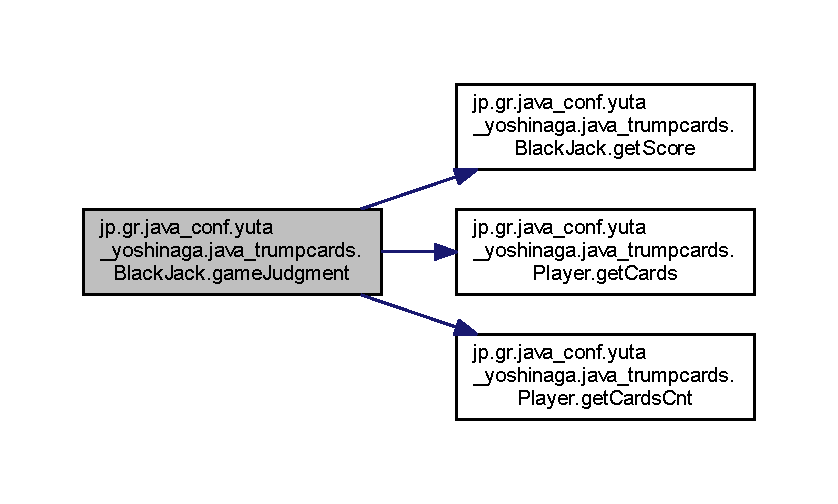
\includegraphics[width=350pt]{classjp_1_1gr_1_1java__conf_1_1yuta__yoshinaga_1_1java__trumpcards_1_1_black_jack_a26f4a11e36c237ec64f08010b8ea0a01_cgraph}
\end{center}
\end{figure}
\mbox{\Hypertarget{classjp_1_1gr_1_1java__conf_1_1yuta__yoshinaga_1_1java__trumpcards_1_1_black_jack_ae3829512336f2ca3f931924b435c8593}\label{classjp_1_1gr_1_1java__conf_1_1yuta__yoshinaga_1_1java__trumpcards_1_1_black_jack_ae3829512336f2ca3f931924b435c8593}} 
\index{jp\+::gr\+::java\+\_\+conf\+::yuta\+\_\+yoshinaga\+::java\+\_\+trumpcards\+::\+Black\+Jack@{jp\+::gr\+::java\+\_\+conf\+::yuta\+\_\+yoshinaga\+::java\+\_\+trumpcards\+::\+Black\+Jack}!get\+Dealer@{get\+Dealer}}
\index{get\+Dealer@{get\+Dealer}!jp\+::gr\+::java\+\_\+conf\+::yuta\+\_\+yoshinaga\+::java\+\_\+trumpcards\+::\+Black\+Jack@{jp\+::gr\+::java\+\_\+conf\+::yuta\+\_\+yoshinaga\+::java\+\_\+trumpcards\+::\+Black\+Jack}}
\subsubsection{\texorpdfstring{get\+Dealer()}{getDealer()}}
{\footnotesize\ttfamily public \hyperlink{classjp_1_1gr_1_1java__conf_1_1yuta__yoshinaga_1_1java__trumpcards_1_1_player}{Player} jp.\+gr.\+java\+\_\+conf.\+yuta\+\_\+yoshinaga.\+java\+\_\+trumpcards.\+Black\+Jack.\+get\+Dealer (\begin{DoxyParamCaption}{ }\end{DoxyParamCaption})}



ゲッター 

\begin{DoxyReturn}{Returns}
ディーラー 
\end{DoxyReturn}
\begin{DoxyAuthor}{Author}
Yuta Yoshinaga 
\end{DoxyAuthor}
\begin{DoxyDate}{Date}
2019.\+04.\+27 
\end{DoxyDate}


Definition at line 106 of file Black\+Jack.\+java.

\mbox{\Hypertarget{classjp_1_1gr_1_1java__conf_1_1yuta__yoshinaga_1_1java__trumpcards_1_1_black_jack_aa541fa5982861610f084bede8c5d6ac1}\label{classjp_1_1gr_1_1java__conf_1_1yuta__yoshinaga_1_1java__trumpcards_1_1_black_jack_aa541fa5982861610f084bede8c5d6ac1}} 
\index{jp\+::gr\+::java\+\_\+conf\+::yuta\+\_\+yoshinaga\+::java\+\_\+trumpcards\+::\+Black\+Jack@{jp\+::gr\+::java\+\_\+conf\+::yuta\+\_\+yoshinaga\+::java\+\_\+trumpcards\+::\+Black\+Jack}!get\+Game\+End\+Flag@{get\+Game\+End\+Flag}}
\index{get\+Game\+End\+Flag@{get\+Game\+End\+Flag}!jp\+::gr\+::java\+\_\+conf\+::yuta\+\_\+yoshinaga\+::java\+\_\+trumpcards\+::\+Black\+Jack@{jp\+::gr\+::java\+\_\+conf\+::yuta\+\_\+yoshinaga\+::java\+\_\+trumpcards\+::\+Black\+Jack}}
\subsubsection{\texorpdfstring{get\+Game\+End\+Flag()}{getGameEndFlag()}}
{\footnotesize\ttfamily public boolean jp.\+gr.\+java\+\_\+conf.\+yuta\+\_\+yoshinaga.\+java\+\_\+trumpcards.\+Black\+Jack.\+get\+Game\+End\+Flag (\begin{DoxyParamCaption}{ }\end{DoxyParamCaption})}



ゲッター 

\begin{DoxyReturn}{Returns}
ディーラー 
\end{DoxyReturn}
\begin{DoxyAuthor}{Author}
Yuta Yoshinaga 
\end{DoxyAuthor}
\begin{DoxyDate}{Date}
2019.\+04.\+27 
\end{DoxyDate}


Definition at line 131 of file Black\+Jack.\+java.

\mbox{\Hypertarget{classjp_1_1gr_1_1java__conf_1_1yuta__yoshinaga_1_1java__trumpcards_1_1_black_jack_aa4fff12d377006ce93d731a6808b67bd}\label{classjp_1_1gr_1_1java__conf_1_1yuta__yoshinaga_1_1java__trumpcards_1_1_black_jack_aa4fff12d377006ce93d731a6808b67bd}} 
\index{jp\+::gr\+::java\+\_\+conf\+::yuta\+\_\+yoshinaga\+::java\+\_\+trumpcards\+::\+Black\+Jack@{jp\+::gr\+::java\+\_\+conf\+::yuta\+\_\+yoshinaga\+::java\+\_\+trumpcards\+::\+Black\+Jack}!get\+Player@{get\+Player}}
\index{get\+Player@{get\+Player}!jp\+::gr\+::java\+\_\+conf\+::yuta\+\_\+yoshinaga\+::java\+\_\+trumpcards\+::\+Black\+Jack@{jp\+::gr\+::java\+\_\+conf\+::yuta\+\_\+yoshinaga\+::java\+\_\+trumpcards\+::\+Black\+Jack}}
\subsubsection{\texorpdfstring{get\+Player()}{getPlayer()}}
{\footnotesize\ttfamily public \hyperlink{classjp_1_1gr_1_1java__conf_1_1yuta__yoshinaga_1_1java__trumpcards_1_1_player}{Player} jp.\+gr.\+java\+\_\+conf.\+yuta\+\_\+yoshinaga.\+java\+\_\+trumpcards.\+Black\+Jack.\+get\+Player (\begin{DoxyParamCaption}{ }\end{DoxyParamCaption})}



ゲッター 

\begin{DoxyReturn}{Returns}
プレイヤー 
\end{DoxyReturn}
\begin{DoxyAuthor}{Author}
Yuta Yoshinaga 
\end{DoxyAuthor}
\begin{DoxyDate}{Date}
2019.\+04.\+27 
\end{DoxyDate}


Definition at line 81 of file Black\+Jack.\+java.

\mbox{\Hypertarget{classjp_1_1gr_1_1java__conf_1_1yuta__yoshinaga_1_1java__trumpcards_1_1_black_jack_a23b680e89ca3a4c306576ba0a7debfac}\label{classjp_1_1gr_1_1java__conf_1_1yuta__yoshinaga_1_1java__trumpcards_1_1_black_jack_a23b680e89ca3a4c306576ba0a7debfac}} 
\index{jp\+::gr\+::java\+\_\+conf\+::yuta\+\_\+yoshinaga\+::java\+\_\+trumpcards\+::\+Black\+Jack@{jp\+::gr\+::java\+\_\+conf\+::yuta\+\_\+yoshinaga\+::java\+\_\+trumpcards\+::\+Black\+Jack}!get\+Score@{get\+Score}}
\index{get\+Score@{get\+Score}!jp\+::gr\+::java\+\_\+conf\+::yuta\+\_\+yoshinaga\+::java\+\_\+trumpcards\+::\+Black\+Jack@{jp\+::gr\+::java\+\_\+conf\+::yuta\+\_\+yoshinaga\+::java\+\_\+trumpcards\+::\+Black\+Jack}}
\subsubsection{\texorpdfstring{get\+Score()}{getScore()}}
{\footnotesize\ttfamily public int jp.\+gr.\+java\+\_\+conf.\+yuta\+\_\+yoshinaga.\+java\+\_\+trumpcards.\+Black\+Jack.\+get\+Score (\begin{DoxyParamCaption}\item[{Array\+List$<$ \hyperlink{classjp_1_1gr_1_1java__conf_1_1yuta__yoshinaga_1_1java__trumpcards_1_1_card}{Card} $>$}]{cards,  }\item[{int}]{cards\+Cnt }\end{DoxyParamCaption})}



手札から現在のスコア取得 


\begin{DoxyParams}[1]{Parameters}
\mbox{\tt in}  & {\em Array\+List$<$\+Card$>$} & cards 手札 \\
\hline
\mbox{\tt in}  & {\em int} & cards\+Cnt 手札枚数 \\
\hline
\end{DoxyParams}
\begin{DoxyReturn}{Returns}
現在のスコア 
\end{DoxyReturn}
\begin{DoxyAuthor}{Author}
Yuta Yoshinaga 
\end{DoxyAuthor}
\begin{DoxyDate}{Date}
2019.\+04.\+27 
\end{DoxyDate}


Definition at line 253 of file Black\+Jack.\+java.



Referenced by jp.\+gr.\+java\+\_\+conf.\+yuta\+\_\+yoshinaga.\+java\+\_\+trumpcards.\+Black\+Jack.\+dealer\+Hit(), jp.\+gr.\+java\+\_\+conf.\+yuta\+\_\+yoshinaga.\+java\+\_\+trumpcards.\+Black\+Jack.\+game\+Judgment(), and jp.\+gr.\+java\+\_\+conf.\+yuta\+\_\+yoshinaga.\+java\+\_\+trumpcards.\+Black\+Jack.\+player\+Hit().

Here is the caller graph for this function\+:
\nopagebreak
\begin{figure}[H]
\begin{center}
\leavevmode
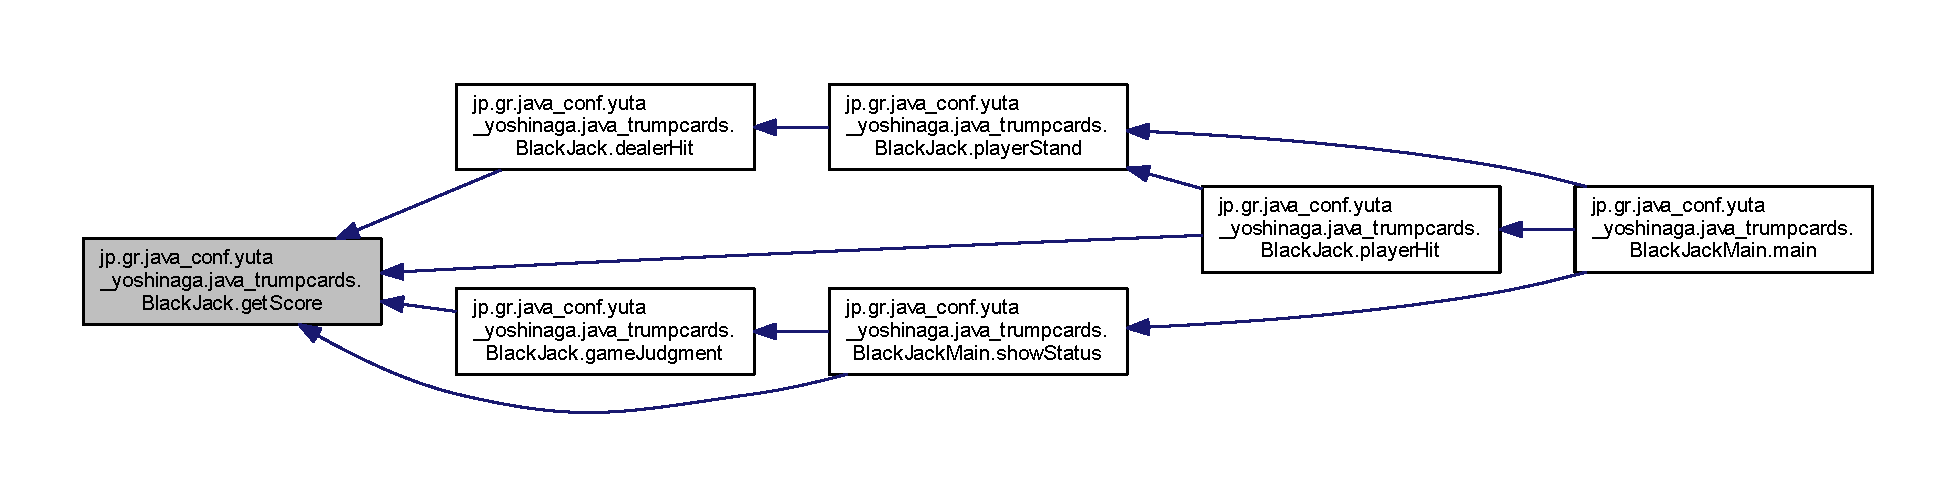
\includegraphics[width=350pt]{classjp_1_1gr_1_1java__conf_1_1yuta__yoshinaga_1_1java__trumpcards_1_1_black_jack_a23b680e89ca3a4c306576ba0a7debfac_icgraph}
\end{center}
\end{figure}
\mbox{\Hypertarget{classjp_1_1gr_1_1java__conf_1_1yuta__yoshinaga_1_1java__trumpcards_1_1_black_jack_a19f0d24ac49d16b9db099801cc6f7340}\label{classjp_1_1gr_1_1java__conf_1_1yuta__yoshinaga_1_1java__trumpcards_1_1_black_jack_a19f0d24ac49d16b9db099801cc6f7340}} 
\index{jp\+::gr\+::java\+\_\+conf\+::yuta\+\_\+yoshinaga\+::java\+\_\+trumpcards\+::\+Black\+Jack@{jp\+::gr\+::java\+\_\+conf\+::yuta\+\_\+yoshinaga\+::java\+\_\+trumpcards\+::\+Black\+Jack}!get\+Trump\+Cards@{get\+Trump\+Cards}}
\index{get\+Trump\+Cards@{get\+Trump\+Cards}!jp\+::gr\+::java\+\_\+conf\+::yuta\+\_\+yoshinaga\+::java\+\_\+trumpcards\+::\+Black\+Jack@{jp\+::gr\+::java\+\_\+conf\+::yuta\+\_\+yoshinaga\+::java\+\_\+trumpcards\+::\+Black\+Jack}}
\subsubsection{\texorpdfstring{get\+Trump\+Cards()}{getTrumpCards()}}
{\footnotesize\ttfamily \hyperlink{classjp_1_1gr_1_1java__conf_1_1yuta__yoshinaga_1_1java__trumpcards_1_1_trump_cards}{Trump\+Cards} jp.\+gr.\+java\+\_\+conf.\+yuta\+\_\+yoshinaga.\+java\+\_\+trumpcards.\+Black\+Jack.\+get\+Trump\+Cards (\begin{DoxyParamCaption}{ }\end{DoxyParamCaption})}



ゲッター 

\begin{DoxyReturn}{Returns}
トランプカード 
\end{DoxyReturn}
\begin{DoxyAuthor}{Author}
Yuta Yoshinaga 
\end{DoxyAuthor}
\begin{DoxyDate}{Date}
2019.\+04.\+27 
\end{DoxyDate}


Definition at line 56 of file Black\+Jack.\+java.

\mbox{\Hypertarget{classjp_1_1gr_1_1java__conf_1_1yuta__yoshinaga_1_1java__trumpcards_1_1_black_jack_a4b8f2248ac868b5d3b9506fb0ece0ea2}\label{classjp_1_1gr_1_1java__conf_1_1yuta__yoshinaga_1_1java__trumpcards_1_1_black_jack_a4b8f2248ac868b5d3b9506fb0ece0ea2}} 
\index{jp\+::gr\+::java\+\_\+conf\+::yuta\+\_\+yoshinaga\+::java\+\_\+trumpcards\+::\+Black\+Jack@{jp\+::gr\+::java\+\_\+conf\+::yuta\+\_\+yoshinaga\+::java\+\_\+trumpcards\+::\+Black\+Jack}!player\+Hit@{player\+Hit}}
\index{player\+Hit@{player\+Hit}!jp\+::gr\+::java\+\_\+conf\+::yuta\+\_\+yoshinaga\+::java\+\_\+trumpcards\+::\+Black\+Jack@{jp\+::gr\+::java\+\_\+conf\+::yuta\+\_\+yoshinaga\+::java\+\_\+trumpcards\+::\+Black\+Jack}}
\subsubsection{\texorpdfstring{player\+Hit()}{playerHit()}}
{\footnotesize\ttfamily public void jp.\+gr.\+java\+\_\+conf.\+yuta\+\_\+yoshinaga.\+java\+\_\+trumpcards.\+Black\+Jack.\+player\+Hit (\begin{DoxyParamCaption}{ }\end{DoxyParamCaption})}



プレイヤーヒット 

\begin{DoxyReturn}{Returns}
ありません 
\end{DoxyReturn}
\begin{DoxyAuthor}{Author}
Yuta Yoshinaga 
\end{DoxyAuthor}
\begin{DoxyDate}{Date}
2019.\+04.\+27 
\end{DoxyDate}


Definition at line 184 of file Black\+Jack.\+java.

Here is the call graph for this function\+:
\nopagebreak
\begin{figure}[H]
\begin{center}
\leavevmode
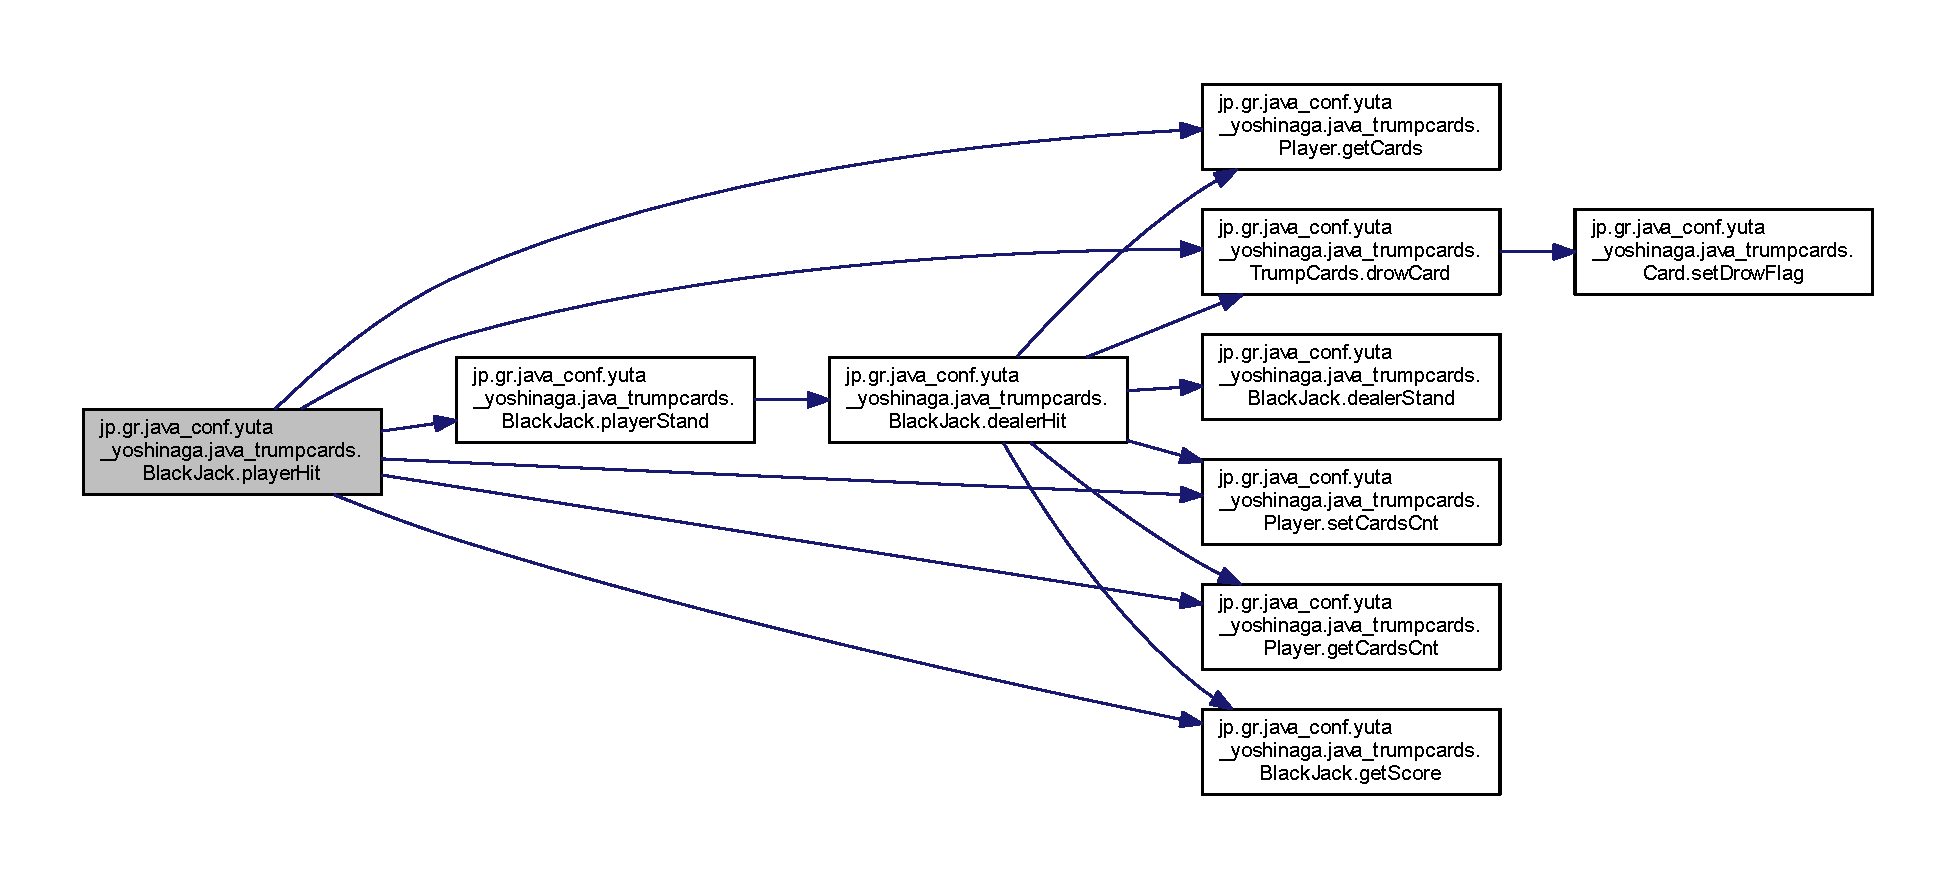
\includegraphics[width=350pt]{classjp_1_1gr_1_1java__conf_1_1yuta__yoshinaga_1_1java__trumpcards_1_1_black_jack_a4b8f2248ac868b5d3b9506fb0ece0ea2_cgraph}
\end{center}
\end{figure}
\mbox{\Hypertarget{classjp_1_1gr_1_1java__conf_1_1yuta__yoshinaga_1_1java__trumpcards_1_1_black_jack_a53f37ae6f1388143c70a8b138c6c2443}\label{classjp_1_1gr_1_1java__conf_1_1yuta__yoshinaga_1_1java__trumpcards_1_1_black_jack_a53f37ae6f1388143c70a8b138c6c2443}} 
\index{jp\+::gr\+::java\+\_\+conf\+::yuta\+\_\+yoshinaga\+::java\+\_\+trumpcards\+::\+Black\+Jack@{jp\+::gr\+::java\+\_\+conf\+::yuta\+\_\+yoshinaga\+::java\+\_\+trumpcards\+::\+Black\+Jack}!player\+Stand@{player\+Stand}}
\index{player\+Stand@{player\+Stand}!jp\+::gr\+::java\+\_\+conf\+::yuta\+\_\+yoshinaga\+::java\+\_\+trumpcards\+::\+Black\+Jack@{jp\+::gr\+::java\+\_\+conf\+::yuta\+\_\+yoshinaga\+::java\+\_\+trumpcards\+::\+Black\+Jack}}
\subsubsection{\texorpdfstring{player\+Stand()}{playerStand()}}
{\footnotesize\ttfamily public void jp.\+gr.\+java\+\_\+conf.\+yuta\+\_\+yoshinaga.\+java\+\_\+trumpcards.\+Black\+Jack.\+player\+Stand (\begin{DoxyParamCaption}{ }\end{DoxyParamCaption})}



プレイヤースタンド 

\begin{DoxyReturn}{Returns}
ありません 
\end{DoxyReturn}
\begin{DoxyAuthor}{Author}
Yuta Yoshinaga 
\end{DoxyAuthor}
\begin{DoxyDate}{Date}
2019.\+04.\+27 
\end{DoxyDate}


Definition at line 202 of file Black\+Jack.\+java.



Referenced by jp.\+gr.\+java\+\_\+conf.\+yuta\+\_\+yoshinaga.\+java\+\_\+trumpcards.\+Black\+Jack.\+player\+Hit().

Here is the call graph for this function\+:
\nopagebreak
\begin{figure}[H]
\begin{center}
\leavevmode
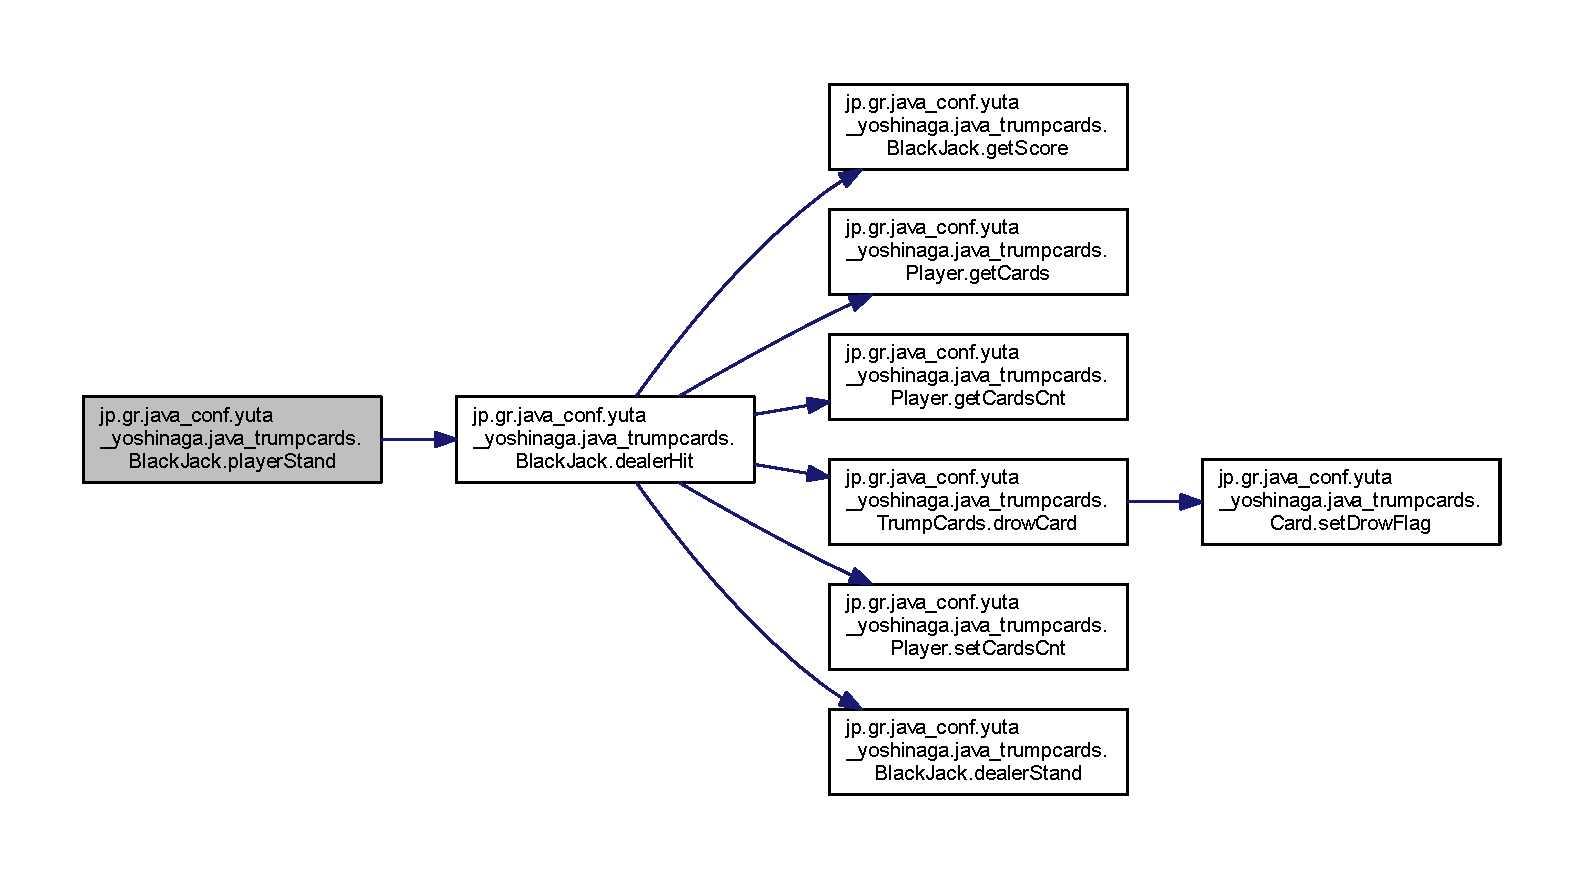
\includegraphics[width=350pt]{classjp_1_1gr_1_1java__conf_1_1yuta__yoshinaga_1_1java__trumpcards_1_1_black_jack_a53f37ae6f1388143c70a8b138c6c2443_cgraph}
\end{center}
\end{figure}
Here is the caller graph for this function\+:
\nopagebreak
\begin{figure}[H]
\begin{center}
\leavevmode
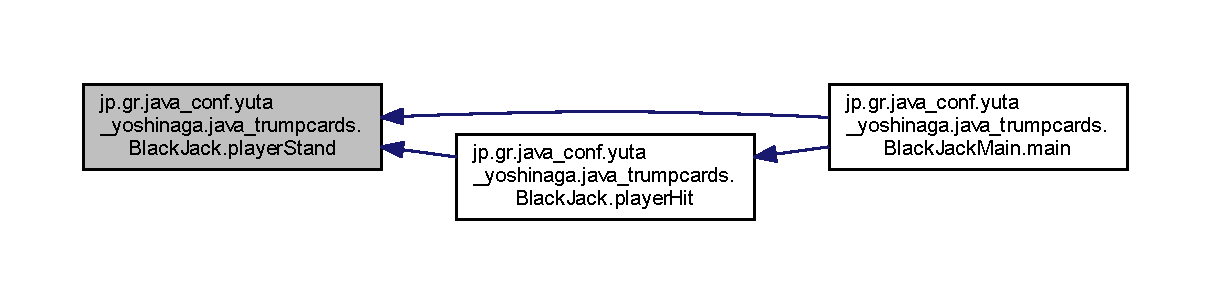
\includegraphics[width=350pt]{classjp_1_1gr_1_1java__conf_1_1yuta__yoshinaga_1_1java__trumpcards_1_1_black_jack_a53f37ae6f1388143c70a8b138c6c2443_icgraph}
\end{center}
\end{figure}
\mbox{\Hypertarget{classjp_1_1gr_1_1java__conf_1_1yuta__yoshinaga_1_1java__trumpcards_1_1_black_jack_a8fd066f80b7dd83f393a770bb24cd675}\label{classjp_1_1gr_1_1java__conf_1_1yuta__yoshinaga_1_1java__trumpcards_1_1_black_jack_a8fd066f80b7dd83f393a770bb24cd675}} 
\index{jp\+::gr\+::java\+\_\+conf\+::yuta\+\_\+yoshinaga\+::java\+\_\+trumpcards\+::\+Black\+Jack@{jp\+::gr\+::java\+\_\+conf\+::yuta\+\_\+yoshinaga\+::java\+\_\+trumpcards\+::\+Black\+Jack}!set\+Dealer@{set\+Dealer}}
\index{set\+Dealer@{set\+Dealer}!jp\+::gr\+::java\+\_\+conf\+::yuta\+\_\+yoshinaga\+::java\+\_\+trumpcards\+::\+Black\+Jack@{jp\+::gr\+::java\+\_\+conf\+::yuta\+\_\+yoshinaga\+::java\+\_\+trumpcards\+::\+Black\+Jack}}
\subsubsection{\texorpdfstring{set\+Dealer()}{setDealer()}}
{\footnotesize\ttfamily public void jp.\+gr.\+java\+\_\+conf.\+yuta\+\_\+yoshinaga.\+java\+\_\+trumpcards.\+Black\+Jack.\+set\+Dealer (\begin{DoxyParamCaption}\item[{\hyperlink{classjp_1_1gr_1_1java__conf_1_1yuta__yoshinaga_1_1java__trumpcards_1_1_player}{Player}}]{dealer }\end{DoxyParamCaption})}



セッター 


\begin{DoxyParams}[1]{Parameters}
\mbox{\tt in}  & {\em \hyperlink{classjp_1_1gr_1_1java__conf_1_1yuta__yoshinaga_1_1java__trumpcards_1_1_player}{Player}} & dealer ディーラー \\
\hline
\end{DoxyParams}
\begin{DoxyReturn}{Returns}
ありません 
\end{DoxyReturn}
\begin{DoxyAuthor}{Author}
Yuta Yoshinaga 
\end{DoxyAuthor}
\begin{DoxyDate}{Date}
2019.\+04.\+27 
\end{DoxyDate}


Definition at line 119 of file Black\+Jack.\+java.

\mbox{\Hypertarget{classjp_1_1gr_1_1java__conf_1_1yuta__yoshinaga_1_1java__trumpcards_1_1_black_jack_a75ef56d0490e7b343fc6c02acbe43dd7}\label{classjp_1_1gr_1_1java__conf_1_1yuta__yoshinaga_1_1java__trumpcards_1_1_black_jack_a75ef56d0490e7b343fc6c02acbe43dd7}} 
\index{jp\+::gr\+::java\+\_\+conf\+::yuta\+\_\+yoshinaga\+::java\+\_\+trumpcards\+::\+Black\+Jack@{jp\+::gr\+::java\+\_\+conf\+::yuta\+\_\+yoshinaga\+::java\+\_\+trumpcards\+::\+Black\+Jack}!set\+Game\+End\+Flag@{set\+Game\+End\+Flag}}
\index{set\+Game\+End\+Flag@{set\+Game\+End\+Flag}!jp\+::gr\+::java\+\_\+conf\+::yuta\+\_\+yoshinaga\+::java\+\_\+trumpcards\+::\+Black\+Jack@{jp\+::gr\+::java\+\_\+conf\+::yuta\+\_\+yoshinaga\+::java\+\_\+trumpcards\+::\+Black\+Jack}}
\subsubsection{\texorpdfstring{set\+Game\+End\+Flag()}{setGameEndFlag()}}
{\footnotesize\ttfamily public void jp.\+gr.\+java\+\_\+conf.\+yuta\+\_\+yoshinaga.\+java\+\_\+trumpcards.\+Black\+Jack.\+set\+Game\+End\+Flag (\begin{DoxyParamCaption}\item[{boolean}]{game\+End\+Flag }\end{DoxyParamCaption})}



セッター 


\begin{DoxyParams}[1]{Parameters}
\mbox{\tt in}  & {\em boolean} & game\+End\+Flag ゲーム終了フラグ \\
\hline
\end{DoxyParams}
\begin{DoxyReturn}{Returns}
ありません 
\end{DoxyReturn}
\begin{DoxyAuthor}{Author}
Yuta Yoshinaga 
\end{DoxyAuthor}
\begin{DoxyDate}{Date}
2019.\+04.\+27 
\end{DoxyDate}


Definition at line 144 of file Black\+Jack.\+java.

\mbox{\Hypertarget{classjp_1_1gr_1_1java__conf_1_1yuta__yoshinaga_1_1java__trumpcards_1_1_black_jack_a3c6bfcfb81ccad65be2f5cfb82819951}\label{classjp_1_1gr_1_1java__conf_1_1yuta__yoshinaga_1_1java__trumpcards_1_1_black_jack_a3c6bfcfb81ccad65be2f5cfb82819951}} 
\index{jp\+::gr\+::java\+\_\+conf\+::yuta\+\_\+yoshinaga\+::java\+\_\+trumpcards\+::\+Black\+Jack@{jp\+::gr\+::java\+\_\+conf\+::yuta\+\_\+yoshinaga\+::java\+\_\+trumpcards\+::\+Black\+Jack}!set\+Player@{set\+Player}}
\index{set\+Player@{set\+Player}!jp\+::gr\+::java\+\_\+conf\+::yuta\+\_\+yoshinaga\+::java\+\_\+trumpcards\+::\+Black\+Jack@{jp\+::gr\+::java\+\_\+conf\+::yuta\+\_\+yoshinaga\+::java\+\_\+trumpcards\+::\+Black\+Jack}}
\subsubsection{\texorpdfstring{set\+Player()}{setPlayer()}}
{\footnotesize\ttfamily public void jp.\+gr.\+java\+\_\+conf.\+yuta\+\_\+yoshinaga.\+java\+\_\+trumpcards.\+Black\+Jack.\+set\+Player (\begin{DoxyParamCaption}\item[{\hyperlink{classjp_1_1gr_1_1java__conf_1_1yuta__yoshinaga_1_1java__trumpcards_1_1_player}{Player}}]{player }\end{DoxyParamCaption})}



セッター 


\begin{DoxyParams}[1]{Parameters}
\mbox{\tt in}  & {\em \hyperlink{classjp_1_1gr_1_1java__conf_1_1yuta__yoshinaga_1_1java__trumpcards_1_1_player}{Player}} & player プレイヤー \\
\hline
\end{DoxyParams}
\begin{DoxyReturn}{Returns}
ありません 
\end{DoxyReturn}
\begin{DoxyAuthor}{Author}
Yuta Yoshinaga 
\end{DoxyAuthor}
\begin{DoxyDate}{Date}
2019.\+04.\+27 
\end{DoxyDate}


Definition at line 94 of file Black\+Jack.\+java.

\mbox{\Hypertarget{classjp_1_1gr_1_1java__conf_1_1yuta__yoshinaga_1_1java__trumpcards_1_1_black_jack_a216185ef3f8c02439b201ec52234aecf}\label{classjp_1_1gr_1_1java__conf_1_1yuta__yoshinaga_1_1java__trumpcards_1_1_black_jack_a216185ef3f8c02439b201ec52234aecf}} 
\index{jp\+::gr\+::java\+\_\+conf\+::yuta\+\_\+yoshinaga\+::java\+\_\+trumpcards\+::\+Black\+Jack@{jp\+::gr\+::java\+\_\+conf\+::yuta\+\_\+yoshinaga\+::java\+\_\+trumpcards\+::\+Black\+Jack}!set\+Trump\+Cards@{set\+Trump\+Cards}}
\index{set\+Trump\+Cards@{set\+Trump\+Cards}!jp\+::gr\+::java\+\_\+conf\+::yuta\+\_\+yoshinaga\+::java\+\_\+trumpcards\+::\+Black\+Jack@{jp\+::gr\+::java\+\_\+conf\+::yuta\+\_\+yoshinaga\+::java\+\_\+trumpcards\+::\+Black\+Jack}}
\subsubsection{\texorpdfstring{set\+Trump\+Cards()}{setTrumpCards()}}
{\footnotesize\ttfamily public void jp.\+gr.\+java\+\_\+conf.\+yuta\+\_\+yoshinaga.\+java\+\_\+trumpcards.\+Black\+Jack.\+set\+Trump\+Cards (\begin{DoxyParamCaption}\item[{\hyperlink{classjp_1_1gr_1_1java__conf_1_1yuta__yoshinaga_1_1java__trumpcards_1_1_trump_cards}{Trump\+Cards}}]{trump\+Cards }\end{DoxyParamCaption})}



セッター 


\begin{DoxyParams}[1]{Parameters}
\mbox{\tt in}  & {\em \hyperlink{classjp_1_1gr_1_1java__conf_1_1yuta__yoshinaga_1_1java__trumpcards_1_1_trump_cards}{Trump\+Cards}} & trump\+Cards トランプカード \\
\hline
\end{DoxyParams}
\begin{DoxyReturn}{Returns}
ありません 
\end{DoxyReturn}
\begin{DoxyAuthor}{Author}
Yuta Yoshinaga 
\end{DoxyAuthor}
\begin{DoxyDate}{Date}
2019.\+04.\+27 
\end{DoxyDate}


Definition at line 69 of file Black\+Jack.\+java.



The documentation for this class was generated from the following file\+:\begin{DoxyCompactItemize}
\item 
jp/gr/java\+\_\+conf/yuta\+\_\+yoshinaga/java\+\_\+trumpcards/\hyperlink{_black_jack_8java}{Black\+Jack.\+java}\end{DoxyCompactItemize}

\hypertarget{classjp_1_1gr_1_1java__conf_1_1yuta__yoshinaga_1_1java__trumpcards_1_1_card}{}\section{jp.\+gr.\+java\+\_\+conf.\+yuta\+\_\+yoshinaga.\+java\+\_\+trumpcards.\+Card Class Reference}
\label{classjp_1_1gr_1_1java__conf_1_1yuta__yoshinaga_1_1java__trumpcards_1_1_card}\index{jp.\+gr.\+java\+\_\+conf.\+yuta\+\_\+yoshinaga.\+java\+\_\+trumpcards.\+Card@{jp.\+gr.\+java\+\_\+conf.\+yuta\+\_\+yoshinaga.\+java\+\_\+trumpcards.\+Card}}


カードクラス  




Collaboration diagram for jp.\+gr.\+java\+\_\+conf.\+yuta\+\_\+yoshinaga.\+java\+\_\+trumpcards.\+Card\+:
\nopagebreak
\begin{figure}[H]
\begin{center}
\leavevmode
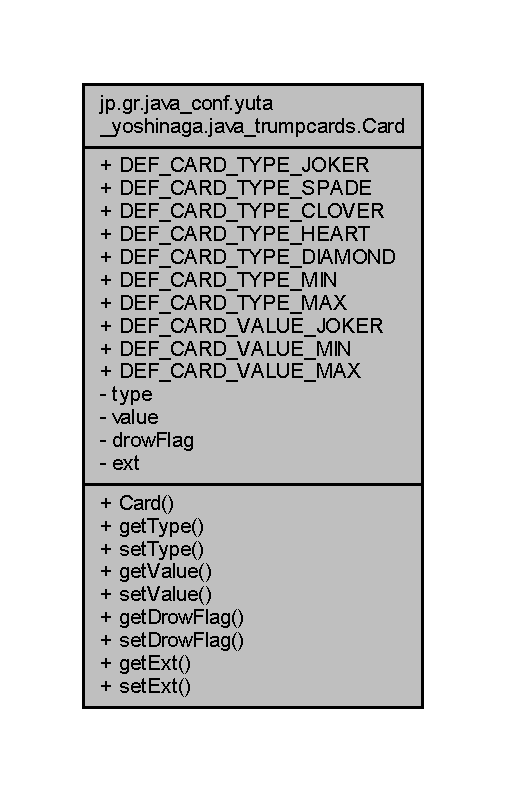
\includegraphics[width=243pt]{classjp_1_1gr_1_1java__conf_1_1yuta__yoshinaga_1_1java__trumpcards_1_1_card__coll__graph}
\end{center}
\end{figure}
\subsection*{Public Member Functions}
\begin{DoxyCompactItemize}
\item 
\hyperlink{classjp_1_1gr_1_1java__conf_1_1yuta__yoshinaga_1_1java__trumpcards_1_1_card_a890c2b43ae091887939cf88c00cc35e6}{Card} ()
\begin{DoxyCompactList}\small\item\em コンストラクタ \end{DoxyCompactList}\item 
int \hyperlink{classjp_1_1gr_1_1java__conf_1_1yuta__yoshinaga_1_1java__trumpcards_1_1_card_a5e3f4e60a101867dfed9db97f417465d}{get\+Type} ()
\begin{DoxyCompactList}\small\item\em ゲッター \end{DoxyCompactList}\item 
void \hyperlink{classjp_1_1gr_1_1java__conf_1_1yuta__yoshinaga_1_1java__trumpcards_1_1_card_a23261f01f6e562e720b5cf55919f1342}{set\+Type} (int \hyperlink{classjp_1_1gr_1_1java__conf_1_1yuta__yoshinaga_1_1java__trumpcards_1_1_card_af77cbc403a7cb0fb5be8610c187e4ff0}{type})
\begin{DoxyCompactList}\small\item\em セッター \end{DoxyCompactList}\item 
int \hyperlink{classjp_1_1gr_1_1java__conf_1_1yuta__yoshinaga_1_1java__trumpcards_1_1_card_aebe71c344f7ef4d1f15d4d30d08898d0}{get\+Value} ()
\begin{DoxyCompactList}\small\item\em ゲッター \end{DoxyCompactList}\item 
void \hyperlink{classjp_1_1gr_1_1java__conf_1_1yuta__yoshinaga_1_1java__trumpcards_1_1_card_a64976287ff631099e8cde6717b1611c6}{set\+Value} (int \hyperlink{classjp_1_1gr_1_1java__conf_1_1yuta__yoshinaga_1_1java__trumpcards_1_1_card_ac71a33a6ef74fca7746b80f02dcd9485}{value})
\begin{DoxyCompactList}\small\item\em セッター \end{DoxyCompactList}\item 
boolean \hyperlink{classjp_1_1gr_1_1java__conf_1_1yuta__yoshinaga_1_1java__trumpcards_1_1_card_a6f9611299599e58a99f53e80e57c1d0c}{get\+Drow\+Flag} ()
\begin{DoxyCompactList}\small\item\em ゲッター \end{DoxyCompactList}\item 
void \hyperlink{classjp_1_1gr_1_1java__conf_1_1yuta__yoshinaga_1_1java__trumpcards_1_1_card_a52e0de709fd788e13ad930562e8e4be2}{set\+Drow\+Flag} (boolean \hyperlink{classjp_1_1gr_1_1java__conf_1_1yuta__yoshinaga_1_1java__trumpcards_1_1_card_a5ea32985f61009d9e2a99733299bc659}{drow\+Flag})
\begin{DoxyCompactList}\small\item\em セッター \end{DoxyCompactList}\item 
String \hyperlink{classjp_1_1gr_1_1java__conf_1_1yuta__yoshinaga_1_1java__trumpcards_1_1_card_ad24d31ccf25cf1eb2ad4304aa5f775cf}{get\+Ext} ()
\begin{DoxyCompactList}\small\item\em ゲッター \end{DoxyCompactList}\item 
void \hyperlink{classjp_1_1gr_1_1java__conf_1_1yuta__yoshinaga_1_1java__trumpcards_1_1_card_a883f9a927c94481d9fd2f3a226499b23}{set\+Ext} (String \hyperlink{classjp_1_1gr_1_1java__conf_1_1yuta__yoshinaga_1_1java__trumpcards_1_1_card_abb47646d84d1b03f3734defbefd32664}{ext})
\begin{DoxyCompactList}\small\item\em セッター \end{DoxyCompactList}\end{DoxyCompactItemize}
\subsection*{Static Public Attributes}
\begin{DoxyCompactItemize}
\item 
\mbox{\Hypertarget{classjp_1_1gr_1_1java__conf_1_1yuta__yoshinaga_1_1java__trumpcards_1_1_card_ae88b4667b9e3b3921267685d1d601799}\label{classjp_1_1gr_1_1java__conf_1_1yuta__yoshinaga_1_1java__trumpcards_1_1_card_ae88b4667b9e3b3921267685d1d601799}} 
static final int {\bfseries D\+E\+F\+\_\+\+C\+A\+R\+D\+\_\+\+T\+Y\+P\+E\+\_\+\+J\+O\+K\+ER} = 0
\item 
\mbox{\Hypertarget{classjp_1_1gr_1_1java__conf_1_1yuta__yoshinaga_1_1java__trumpcards_1_1_card_afdfc14b6408462a614e512b1329327f6}\label{classjp_1_1gr_1_1java__conf_1_1yuta__yoshinaga_1_1java__trumpcards_1_1_card_afdfc14b6408462a614e512b1329327f6}} 
static final int {\bfseries D\+E\+F\+\_\+\+C\+A\+R\+D\+\_\+\+T\+Y\+P\+E\+\_\+\+S\+P\+A\+DE} = 1
\item 
\mbox{\Hypertarget{classjp_1_1gr_1_1java__conf_1_1yuta__yoshinaga_1_1java__trumpcards_1_1_card_a4286dd64dc393577368e71a1c969a14a}\label{classjp_1_1gr_1_1java__conf_1_1yuta__yoshinaga_1_1java__trumpcards_1_1_card_a4286dd64dc393577368e71a1c969a14a}} 
static final int {\bfseries D\+E\+F\+\_\+\+C\+A\+R\+D\+\_\+\+T\+Y\+P\+E\+\_\+\+C\+L\+O\+V\+ER} = 2
\item 
\mbox{\Hypertarget{classjp_1_1gr_1_1java__conf_1_1yuta__yoshinaga_1_1java__trumpcards_1_1_card_a8c257e8baa0cf6dce69a386e869e4c81}\label{classjp_1_1gr_1_1java__conf_1_1yuta__yoshinaga_1_1java__trumpcards_1_1_card_a8c257e8baa0cf6dce69a386e869e4c81}} 
static final int {\bfseries D\+E\+F\+\_\+\+C\+A\+R\+D\+\_\+\+T\+Y\+P\+E\+\_\+\+H\+E\+A\+RT} = 3
\item 
\mbox{\Hypertarget{classjp_1_1gr_1_1java__conf_1_1yuta__yoshinaga_1_1java__trumpcards_1_1_card_a3461c036ef26d9444ff4d7f8a21266a7}\label{classjp_1_1gr_1_1java__conf_1_1yuta__yoshinaga_1_1java__trumpcards_1_1_card_a3461c036ef26d9444ff4d7f8a21266a7}} 
static final int {\bfseries D\+E\+F\+\_\+\+C\+A\+R\+D\+\_\+\+T\+Y\+P\+E\+\_\+\+D\+I\+A\+M\+O\+ND} = 4
\item 
\mbox{\Hypertarget{classjp_1_1gr_1_1java__conf_1_1yuta__yoshinaga_1_1java__trumpcards_1_1_card_a82273fbdd1db45d311f6200597d8b2ff}\label{classjp_1_1gr_1_1java__conf_1_1yuta__yoshinaga_1_1java__trumpcards_1_1_card_a82273fbdd1db45d311f6200597d8b2ff}} 
static final int {\bfseries D\+E\+F\+\_\+\+C\+A\+R\+D\+\_\+\+T\+Y\+P\+E\+\_\+\+M\+IN} = D\+E\+F\+\_\+\+C\+A\+R\+D\+\_\+\+T\+Y\+P\+E\+\_\+\+J\+O\+K\+ER
\item 
\mbox{\Hypertarget{classjp_1_1gr_1_1java__conf_1_1yuta__yoshinaga_1_1java__trumpcards_1_1_card_aaffc3842efef34252ff6a57fb5ffef3c}\label{classjp_1_1gr_1_1java__conf_1_1yuta__yoshinaga_1_1java__trumpcards_1_1_card_aaffc3842efef34252ff6a57fb5ffef3c}} 
static final int {\bfseries D\+E\+F\+\_\+\+C\+A\+R\+D\+\_\+\+T\+Y\+P\+E\+\_\+\+M\+AX} = D\+E\+F\+\_\+\+C\+A\+R\+D\+\_\+\+T\+Y\+P\+E\+\_\+\+D\+I\+A\+M\+O\+ND
\item 
\mbox{\Hypertarget{classjp_1_1gr_1_1java__conf_1_1yuta__yoshinaga_1_1java__trumpcards_1_1_card_a319a77c902355f19915e7c843f3d89f6}\label{classjp_1_1gr_1_1java__conf_1_1yuta__yoshinaga_1_1java__trumpcards_1_1_card_a319a77c902355f19915e7c843f3d89f6}} 
static final int {\bfseries D\+E\+F\+\_\+\+C\+A\+R\+D\+\_\+\+V\+A\+L\+U\+E\+\_\+\+J\+O\+K\+ER} = 0
\item 
\mbox{\Hypertarget{classjp_1_1gr_1_1java__conf_1_1yuta__yoshinaga_1_1java__trumpcards_1_1_card_af7c535700f9899134c0361a4a782ed6f}\label{classjp_1_1gr_1_1java__conf_1_1yuta__yoshinaga_1_1java__trumpcards_1_1_card_af7c535700f9899134c0361a4a782ed6f}} 
static final int {\bfseries D\+E\+F\+\_\+\+C\+A\+R\+D\+\_\+\+V\+A\+L\+U\+E\+\_\+\+M\+IN} = 0
\item 
\mbox{\Hypertarget{classjp_1_1gr_1_1java__conf_1_1yuta__yoshinaga_1_1java__trumpcards_1_1_card_abe13d7fb6cfdf0454cb85d449b294893}\label{classjp_1_1gr_1_1java__conf_1_1yuta__yoshinaga_1_1java__trumpcards_1_1_card_abe13d7fb6cfdf0454cb85d449b294893}} 
static final int {\bfseries D\+E\+F\+\_\+\+C\+A\+R\+D\+\_\+\+V\+A\+L\+U\+E\+\_\+\+M\+AX} = 13
\end{DoxyCompactItemize}
\subsection*{Private Attributes}
\begin{DoxyCompactItemize}
\item 
\mbox{\Hypertarget{classjp_1_1gr_1_1java__conf_1_1yuta__yoshinaga_1_1java__trumpcards_1_1_card_af77cbc403a7cb0fb5be8610c187e4ff0}\label{classjp_1_1gr_1_1java__conf_1_1yuta__yoshinaga_1_1java__trumpcards_1_1_card_af77cbc403a7cb0fb5be8610c187e4ff0}} 
int \hyperlink{classjp_1_1gr_1_1java__conf_1_1yuta__yoshinaga_1_1java__trumpcards_1_1_card_af77cbc403a7cb0fb5be8610c187e4ff0}{type}
\begin{DoxyCompactList}\small\item\em カード種類 \end{DoxyCompactList}\item 
\mbox{\Hypertarget{classjp_1_1gr_1_1java__conf_1_1yuta__yoshinaga_1_1java__trumpcards_1_1_card_ac71a33a6ef74fca7746b80f02dcd9485}\label{classjp_1_1gr_1_1java__conf_1_1yuta__yoshinaga_1_1java__trumpcards_1_1_card_ac71a33a6ef74fca7746b80f02dcd9485}} 
int \hyperlink{classjp_1_1gr_1_1java__conf_1_1yuta__yoshinaga_1_1java__trumpcards_1_1_card_ac71a33a6ef74fca7746b80f02dcd9485}{value}
\begin{DoxyCompactList}\small\item\em カード値 \end{DoxyCompactList}\item 
\mbox{\Hypertarget{classjp_1_1gr_1_1java__conf_1_1yuta__yoshinaga_1_1java__trumpcards_1_1_card_a5ea32985f61009d9e2a99733299bc659}\label{classjp_1_1gr_1_1java__conf_1_1yuta__yoshinaga_1_1java__trumpcards_1_1_card_a5ea32985f61009d9e2a99733299bc659}} 
boolean \hyperlink{classjp_1_1gr_1_1java__conf_1_1yuta__yoshinaga_1_1java__trumpcards_1_1_card_a5ea32985f61009d9e2a99733299bc659}{drow\+Flag}
\begin{DoxyCompactList}\small\item\em カード払い出しフラグ \end{DoxyCompactList}\item 
\mbox{\Hypertarget{classjp_1_1gr_1_1java__conf_1_1yuta__yoshinaga_1_1java__trumpcards_1_1_card_abb47646d84d1b03f3734defbefd32664}\label{classjp_1_1gr_1_1java__conf_1_1yuta__yoshinaga_1_1java__trumpcards_1_1_card_abb47646d84d1b03f3734defbefd32664}} 
String \hyperlink{classjp_1_1gr_1_1java__conf_1_1yuta__yoshinaga_1_1java__trumpcards_1_1_card_abb47646d84d1b03f3734defbefd32664}{ext}
\begin{DoxyCompactList}\small\item\em カード拡張情報など(カード別にメッセージを出す場合など) \end{DoxyCompactList}\end{DoxyCompactItemize}


\subsection{Detailed Description}
カードクラス 

Definition at line 25 of file Card.\+java.



\subsection{Constructor \& Destructor Documentation}
\mbox{\Hypertarget{classjp_1_1gr_1_1java__conf_1_1yuta__yoshinaga_1_1java__trumpcards_1_1_card_a890c2b43ae091887939cf88c00cc35e6}\label{classjp_1_1gr_1_1java__conf_1_1yuta__yoshinaga_1_1java__trumpcards_1_1_card_a890c2b43ae091887939cf88c00cc35e6}} 
\index{jp\+::gr\+::java\+\_\+conf\+::yuta\+\_\+yoshinaga\+::java\+\_\+trumpcards\+::\+Card@{jp\+::gr\+::java\+\_\+conf\+::yuta\+\_\+yoshinaga\+::java\+\_\+trumpcards\+::\+Card}!Card@{Card}}
\index{Card@{Card}!jp\+::gr\+::java\+\_\+conf\+::yuta\+\_\+yoshinaga\+::java\+\_\+trumpcards\+::\+Card@{jp\+::gr\+::java\+\_\+conf\+::yuta\+\_\+yoshinaga\+::java\+\_\+trumpcards\+::\+Card}}
\subsubsection{\texorpdfstring{Card()}{Card()}}
{\footnotesize\ttfamily public jp.\+gr.\+java\+\_\+conf.\+yuta\+\_\+yoshinaga.\+java\+\_\+trumpcards.\+Card.\+Card (\begin{DoxyParamCaption}{ }\end{DoxyParamCaption})}



コンストラクタ 

\begin{DoxyReturn}{Returns}
ありません 
\end{DoxyReturn}
\begin{DoxyAuthor}{Author}
Yuta Yoshinaga 
\end{DoxyAuthor}
\begin{DoxyDate}{Date}
2019.\+04.\+27 
\end{DoxyDate}


Definition at line 51 of file Card.\+java.



\subsection{Member Function Documentation}
\mbox{\Hypertarget{classjp_1_1gr_1_1java__conf_1_1yuta__yoshinaga_1_1java__trumpcards_1_1_card_a6f9611299599e58a99f53e80e57c1d0c}\label{classjp_1_1gr_1_1java__conf_1_1yuta__yoshinaga_1_1java__trumpcards_1_1_card_a6f9611299599e58a99f53e80e57c1d0c}} 
\index{jp\+::gr\+::java\+\_\+conf\+::yuta\+\_\+yoshinaga\+::java\+\_\+trumpcards\+::\+Card@{jp\+::gr\+::java\+\_\+conf\+::yuta\+\_\+yoshinaga\+::java\+\_\+trumpcards\+::\+Card}!get\+Drow\+Flag@{get\+Drow\+Flag}}
\index{get\+Drow\+Flag@{get\+Drow\+Flag}!jp\+::gr\+::java\+\_\+conf\+::yuta\+\_\+yoshinaga\+::java\+\_\+trumpcards\+::\+Card@{jp\+::gr\+::java\+\_\+conf\+::yuta\+\_\+yoshinaga\+::java\+\_\+trumpcards\+::\+Card}}
\subsubsection{\texorpdfstring{get\+Drow\+Flag()}{getDrowFlag()}}
{\footnotesize\ttfamily public boolean jp.\+gr.\+java\+\_\+conf.\+yuta\+\_\+yoshinaga.\+java\+\_\+trumpcards.\+Card.\+get\+Drow\+Flag (\begin{DoxyParamCaption}{ }\end{DoxyParamCaption})}



ゲッター 

\begin{DoxyReturn}{Returns}
カード払い出しフラグ 
\end{DoxyReturn}
\begin{DoxyAuthor}{Author}
Yuta Yoshinaga 
\end{DoxyAuthor}
\begin{DoxyDate}{Date}
2019.\+04.\+27 
\end{DoxyDate}


Definition at line 120 of file Card.\+java.

\mbox{\Hypertarget{classjp_1_1gr_1_1java__conf_1_1yuta__yoshinaga_1_1java__trumpcards_1_1_card_ad24d31ccf25cf1eb2ad4304aa5f775cf}\label{classjp_1_1gr_1_1java__conf_1_1yuta__yoshinaga_1_1java__trumpcards_1_1_card_ad24d31ccf25cf1eb2ad4304aa5f775cf}} 
\index{jp\+::gr\+::java\+\_\+conf\+::yuta\+\_\+yoshinaga\+::java\+\_\+trumpcards\+::\+Card@{jp\+::gr\+::java\+\_\+conf\+::yuta\+\_\+yoshinaga\+::java\+\_\+trumpcards\+::\+Card}!get\+Ext@{get\+Ext}}
\index{get\+Ext@{get\+Ext}!jp\+::gr\+::java\+\_\+conf\+::yuta\+\_\+yoshinaga\+::java\+\_\+trumpcards\+::\+Card@{jp\+::gr\+::java\+\_\+conf\+::yuta\+\_\+yoshinaga\+::java\+\_\+trumpcards\+::\+Card}}
\subsubsection{\texorpdfstring{get\+Ext()}{getExt()}}
{\footnotesize\ttfamily public String jp.\+gr.\+java\+\_\+conf.\+yuta\+\_\+yoshinaga.\+java\+\_\+trumpcards.\+Card.\+get\+Ext (\begin{DoxyParamCaption}{ }\end{DoxyParamCaption})}



ゲッター 

\begin{DoxyReturn}{Returns}
カード払い出しフラグ 
\end{DoxyReturn}
\begin{DoxyAuthor}{Author}
Yuta Yoshinaga 
\end{DoxyAuthor}
\begin{DoxyDate}{Date}
2019.\+04.\+27 
\end{DoxyDate}


Definition at line 145 of file Card.\+java.

\mbox{\Hypertarget{classjp_1_1gr_1_1java__conf_1_1yuta__yoshinaga_1_1java__trumpcards_1_1_card_a5e3f4e60a101867dfed9db97f417465d}\label{classjp_1_1gr_1_1java__conf_1_1yuta__yoshinaga_1_1java__trumpcards_1_1_card_a5e3f4e60a101867dfed9db97f417465d}} 
\index{jp\+::gr\+::java\+\_\+conf\+::yuta\+\_\+yoshinaga\+::java\+\_\+trumpcards\+::\+Card@{jp\+::gr\+::java\+\_\+conf\+::yuta\+\_\+yoshinaga\+::java\+\_\+trumpcards\+::\+Card}!get\+Type@{get\+Type}}
\index{get\+Type@{get\+Type}!jp\+::gr\+::java\+\_\+conf\+::yuta\+\_\+yoshinaga\+::java\+\_\+trumpcards\+::\+Card@{jp\+::gr\+::java\+\_\+conf\+::yuta\+\_\+yoshinaga\+::java\+\_\+trumpcards\+::\+Card}}
\subsubsection{\texorpdfstring{get\+Type()}{getType()}}
{\footnotesize\ttfamily public int jp.\+gr.\+java\+\_\+conf.\+yuta\+\_\+yoshinaga.\+java\+\_\+trumpcards.\+Card.\+get\+Type (\begin{DoxyParamCaption}{ }\end{DoxyParamCaption})}



ゲッター 

\begin{DoxyReturn}{Returns}
カード種類 
\end{DoxyReturn}
\begin{DoxyAuthor}{Author}
Yuta Yoshinaga 
\end{DoxyAuthor}
\begin{DoxyDate}{Date}
2019.\+04.\+27 
\end{DoxyDate}


Definition at line 66 of file Card.\+java.



Referenced by jp.\+gr.\+java\+\_\+conf.\+yuta\+\_\+yoshinaga.\+java\+\_\+trumpcards.\+Black\+Jack\+Main.\+get\+Card\+Str().

Here is the caller graph for this function\+:
\nopagebreak
\begin{figure}[H]
\begin{center}
\leavevmode
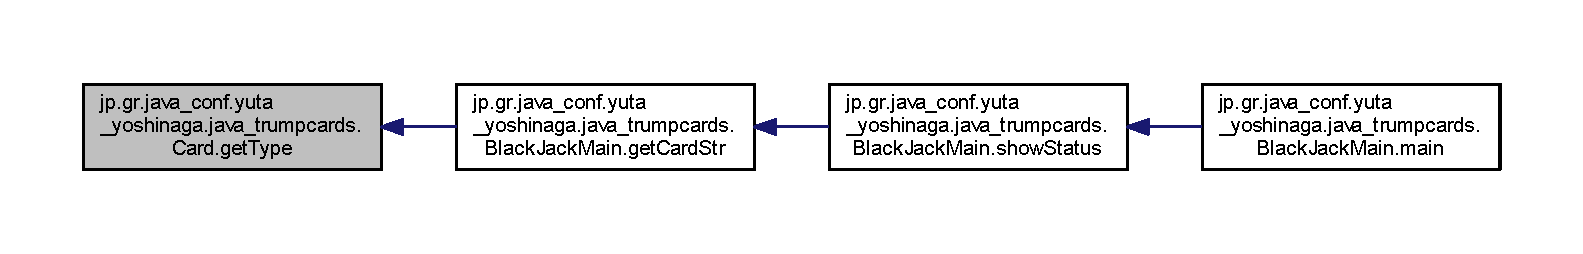
\includegraphics[width=350pt]{classjp_1_1gr_1_1java__conf_1_1yuta__yoshinaga_1_1java__trumpcards_1_1_card_a5e3f4e60a101867dfed9db97f417465d_icgraph}
\end{center}
\end{figure}
\mbox{\Hypertarget{classjp_1_1gr_1_1java__conf_1_1yuta__yoshinaga_1_1java__trumpcards_1_1_card_aebe71c344f7ef4d1f15d4d30d08898d0}\label{classjp_1_1gr_1_1java__conf_1_1yuta__yoshinaga_1_1java__trumpcards_1_1_card_aebe71c344f7ef4d1f15d4d30d08898d0}} 
\index{jp\+::gr\+::java\+\_\+conf\+::yuta\+\_\+yoshinaga\+::java\+\_\+trumpcards\+::\+Card@{jp\+::gr\+::java\+\_\+conf\+::yuta\+\_\+yoshinaga\+::java\+\_\+trumpcards\+::\+Card}!get\+Value@{get\+Value}}
\index{get\+Value@{get\+Value}!jp\+::gr\+::java\+\_\+conf\+::yuta\+\_\+yoshinaga\+::java\+\_\+trumpcards\+::\+Card@{jp\+::gr\+::java\+\_\+conf\+::yuta\+\_\+yoshinaga\+::java\+\_\+trumpcards\+::\+Card}}
\subsubsection{\texorpdfstring{get\+Value()}{getValue()}}
{\footnotesize\ttfamily public jp.\+gr.\+java\+\_\+conf.\+yuta\+\_\+yoshinaga.\+java\+\_\+trumpcards.\+Card.\+get\+Value (\begin{DoxyParamCaption}{ }\end{DoxyParamCaption})}



ゲッター 

\begin{DoxyReturn}{Returns}
カード値 
\end{DoxyReturn}
\begin{DoxyAuthor}{Author}
Yuta Yoshinaga 
\end{DoxyAuthor}
\begin{DoxyDate}{Date}
2019.\+04.\+27 
\end{DoxyDate}


Definition at line 93 of file Card.\+java.



Referenced by jp.\+gr.\+java\+\_\+conf.\+yuta\+\_\+yoshinaga.\+java\+\_\+trumpcards.\+Black\+Jack\+Main.\+get\+Card\+Str().

Here is the caller graph for this function\+:
\nopagebreak
\begin{figure}[H]
\begin{center}
\leavevmode
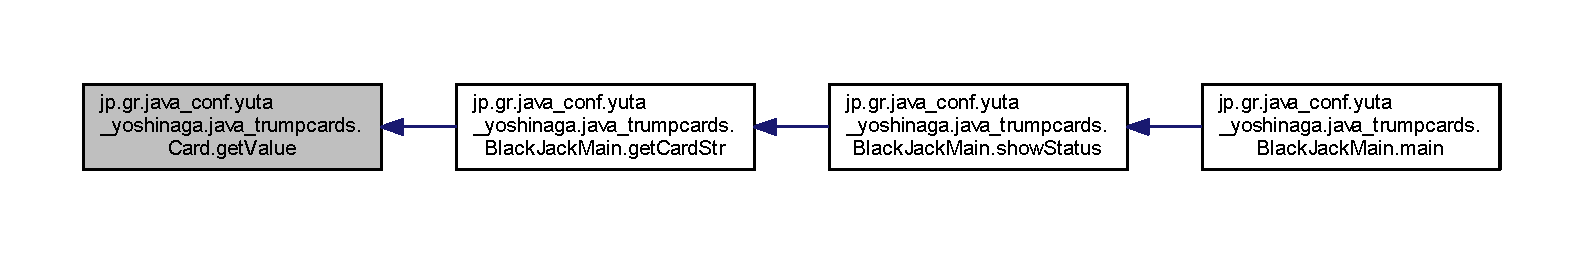
\includegraphics[width=350pt]{classjp_1_1gr_1_1java__conf_1_1yuta__yoshinaga_1_1java__trumpcards_1_1_card_aebe71c344f7ef4d1f15d4d30d08898d0_icgraph}
\end{center}
\end{figure}
\mbox{\Hypertarget{classjp_1_1gr_1_1java__conf_1_1yuta__yoshinaga_1_1java__trumpcards_1_1_card_a52e0de709fd788e13ad930562e8e4be2}\label{classjp_1_1gr_1_1java__conf_1_1yuta__yoshinaga_1_1java__trumpcards_1_1_card_a52e0de709fd788e13ad930562e8e4be2}} 
\index{jp\+::gr\+::java\+\_\+conf\+::yuta\+\_\+yoshinaga\+::java\+\_\+trumpcards\+::\+Card@{jp\+::gr\+::java\+\_\+conf\+::yuta\+\_\+yoshinaga\+::java\+\_\+trumpcards\+::\+Card}!set\+Drow\+Flag@{set\+Drow\+Flag}}
\index{set\+Drow\+Flag@{set\+Drow\+Flag}!jp\+::gr\+::java\+\_\+conf\+::yuta\+\_\+yoshinaga\+::java\+\_\+trumpcards\+::\+Card@{jp\+::gr\+::java\+\_\+conf\+::yuta\+\_\+yoshinaga\+::java\+\_\+trumpcards\+::\+Card}}
\subsubsection{\texorpdfstring{set\+Drow\+Flag()}{setDrowFlag()}}
{\footnotesize\ttfamily public void jp.\+gr.\+java\+\_\+conf.\+yuta\+\_\+yoshinaga.\+java\+\_\+trumpcards.\+Card.\+set\+Drow\+Flag (\begin{DoxyParamCaption}\item[{boolean}]{drow\+Flag }\end{DoxyParamCaption})}



セッター 


\begin{DoxyParams}[1]{Parameters}
\mbox{\tt in}  & {\em boolean} & drow\+Flag カード払い出しフラグ \\
\hline
\end{DoxyParams}
\begin{DoxyReturn}{Returns}
ありません 
\end{DoxyReturn}
\begin{DoxyAuthor}{Author}
Yuta Yoshinaga 
\end{DoxyAuthor}
\begin{DoxyDate}{Date}
2019.\+04.\+27 
\end{DoxyDate}


Definition at line 133 of file Card.\+java.



Referenced by jp.\+gr.\+java\+\_\+conf.\+yuta\+\_\+yoshinaga.\+java\+\_\+trumpcards.\+Trump\+Cards.\+cards\+Init(), and jp.\+gr.\+java\+\_\+conf.\+yuta\+\_\+yoshinaga.\+java\+\_\+trumpcards.\+Trump\+Cards.\+drow\+Card().

Here is the caller graph for this function\+:
\nopagebreak
\begin{figure}[H]
\begin{center}
\leavevmode
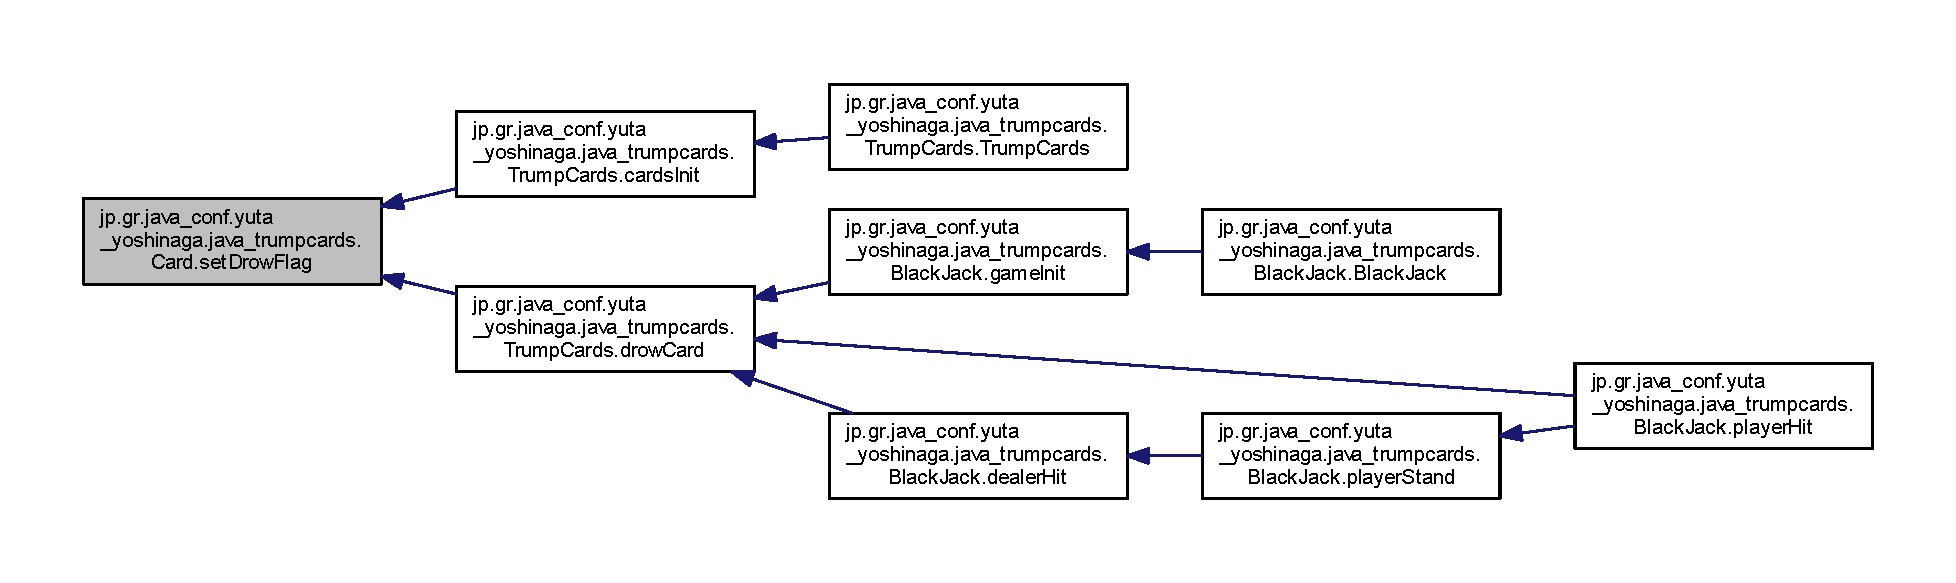
\includegraphics[width=350pt]{classjp_1_1gr_1_1java__conf_1_1yuta__yoshinaga_1_1java__trumpcards_1_1_card_a52e0de709fd788e13ad930562e8e4be2_icgraph}
\end{center}
\end{figure}
\mbox{\Hypertarget{classjp_1_1gr_1_1java__conf_1_1yuta__yoshinaga_1_1java__trumpcards_1_1_card_a883f9a927c94481d9fd2f3a226499b23}\label{classjp_1_1gr_1_1java__conf_1_1yuta__yoshinaga_1_1java__trumpcards_1_1_card_a883f9a927c94481d9fd2f3a226499b23}} 
\index{jp\+::gr\+::java\+\_\+conf\+::yuta\+\_\+yoshinaga\+::java\+\_\+trumpcards\+::\+Card@{jp\+::gr\+::java\+\_\+conf\+::yuta\+\_\+yoshinaga\+::java\+\_\+trumpcards\+::\+Card}!set\+Ext@{set\+Ext}}
\index{set\+Ext@{set\+Ext}!jp\+::gr\+::java\+\_\+conf\+::yuta\+\_\+yoshinaga\+::java\+\_\+trumpcards\+::\+Card@{jp\+::gr\+::java\+\_\+conf\+::yuta\+\_\+yoshinaga\+::java\+\_\+trumpcards\+::\+Card}}
\subsubsection{\texorpdfstring{set\+Ext()}{setExt()}}
{\footnotesize\ttfamily public void jp.\+gr.\+java\+\_\+conf.\+yuta\+\_\+yoshinaga.\+java\+\_\+trumpcards.\+Card.\+set\+Ext (\begin{DoxyParamCaption}\item[{String}]{ext }\end{DoxyParamCaption})}



セッター 


\begin{DoxyParams}[1]{Parameters}
\mbox{\tt in}  & {\em String} & ext カード拡張情報など(カード別にメッセージを出す場合など) \\
\hline
\end{DoxyParams}
\begin{DoxyReturn}{Returns}
ありません 
\end{DoxyReturn}
\begin{DoxyAuthor}{Author}
Yuta Yoshinaga 
\end{DoxyAuthor}
\begin{DoxyDate}{Date}
2019.\+04.\+27 
\end{DoxyDate}


Definition at line 158 of file Card.\+java.

\mbox{\Hypertarget{classjp_1_1gr_1_1java__conf_1_1yuta__yoshinaga_1_1java__trumpcards_1_1_card_a23261f01f6e562e720b5cf55919f1342}\label{classjp_1_1gr_1_1java__conf_1_1yuta__yoshinaga_1_1java__trumpcards_1_1_card_a23261f01f6e562e720b5cf55919f1342}} 
\index{jp\+::gr\+::java\+\_\+conf\+::yuta\+\_\+yoshinaga\+::java\+\_\+trumpcards\+::\+Card@{jp\+::gr\+::java\+\_\+conf\+::yuta\+\_\+yoshinaga\+::java\+\_\+trumpcards\+::\+Card}!set\+Type@{set\+Type}}
\index{set\+Type@{set\+Type}!jp\+::gr\+::java\+\_\+conf\+::yuta\+\_\+yoshinaga\+::java\+\_\+trumpcards\+::\+Card@{jp\+::gr\+::java\+\_\+conf\+::yuta\+\_\+yoshinaga\+::java\+\_\+trumpcards\+::\+Card}}
\subsubsection{\texorpdfstring{set\+Type()}{setType()}}
{\footnotesize\ttfamily public void jp.\+gr.\+java\+\_\+conf.\+yuta\+\_\+yoshinaga.\+java\+\_\+trumpcards.\+Card.\+set\+Type (\begin{DoxyParamCaption}\item[{int}]{type }\end{DoxyParamCaption})}



セッター 


\begin{DoxyParams}[1]{Parameters}
\mbox{\tt in}  & {\em int} & type カード種類 \\
\hline
\end{DoxyParams}
\begin{DoxyReturn}{Returns}
ありません 
\end{DoxyReturn}
\begin{DoxyAuthor}{Author}
Yuta Yoshinaga 
\end{DoxyAuthor}
\begin{DoxyDate}{Date}
2019.\+04.\+27 
\end{DoxyDate}


Definition at line 79 of file Card.\+java.



Referenced by jp.\+gr.\+java\+\_\+conf.\+yuta\+\_\+yoshinaga.\+java\+\_\+trumpcards.\+Trump\+Cards.\+cards\+Init().

Here is the caller graph for this function\+:
\nopagebreak
\begin{figure}[H]
\begin{center}
\leavevmode
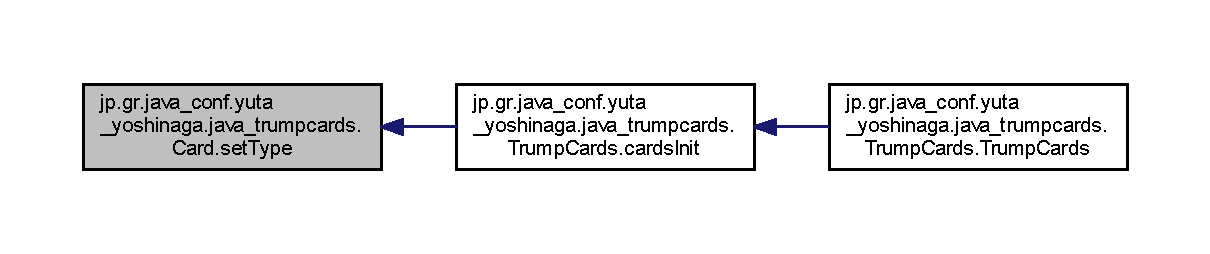
\includegraphics[width=350pt]{classjp_1_1gr_1_1java__conf_1_1yuta__yoshinaga_1_1java__trumpcards_1_1_card_a23261f01f6e562e720b5cf55919f1342_icgraph}
\end{center}
\end{figure}
\mbox{\Hypertarget{classjp_1_1gr_1_1java__conf_1_1yuta__yoshinaga_1_1java__trumpcards_1_1_card_a64976287ff631099e8cde6717b1611c6}\label{classjp_1_1gr_1_1java__conf_1_1yuta__yoshinaga_1_1java__trumpcards_1_1_card_a64976287ff631099e8cde6717b1611c6}} 
\index{jp\+::gr\+::java\+\_\+conf\+::yuta\+\_\+yoshinaga\+::java\+\_\+trumpcards\+::\+Card@{jp\+::gr\+::java\+\_\+conf\+::yuta\+\_\+yoshinaga\+::java\+\_\+trumpcards\+::\+Card}!set\+Value@{set\+Value}}
\index{set\+Value@{set\+Value}!jp\+::gr\+::java\+\_\+conf\+::yuta\+\_\+yoshinaga\+::java\+\_\+trumpcards\+::\+Card@{jp\+::gr\+::java\+\_\+conf\+::yuta\+\_\+yoshinaga\+::java\+\_\+trumpcards\+::\+Card}}
\subsubsection{\texorpdfstring{set\+Value()}{setValue()}}
{\footnotesize\ttfamily public void jp.\+gr.\+java\+\_\+conf.\+yuta\+\_\+yoshinaga.\+java\+\_\+trumpcards.\+Card.\+set\+Value (\begin{DoxyParamCaption}\item[{int}]{value }\end{DoxyParamCaption})}



セッター 


\begin{DoxyParams}[1]{Parameters}
\mbox{\tt in}  & {\em int} & value カード値 \\
\hline
\end{DoxyParams}
\begin{DoxyReturn}{Returns}
ありません 
\end{DoxyReturn}
\begin{DoxyAuthor}{Author}
Yuta Yoshinaga 
\end{DoxyAuthor}
\begin{DoxyDate}{Date}
2019.\+04.\+27 
\end{DoxyDate}


Definition at line 106 of file Card.\+java.



Referenced by jp.\+gr.\+java\+\_\+conf.\+yuta\+\_\+yoshinaga.\+java\+\_\+trumpcards.\+Trump\+Cards.\+cards\+Init().

Here is the caller graph for this function\+:
\nopagebreak
\begin{figure}[H]
\begin{center}
\leavevmode
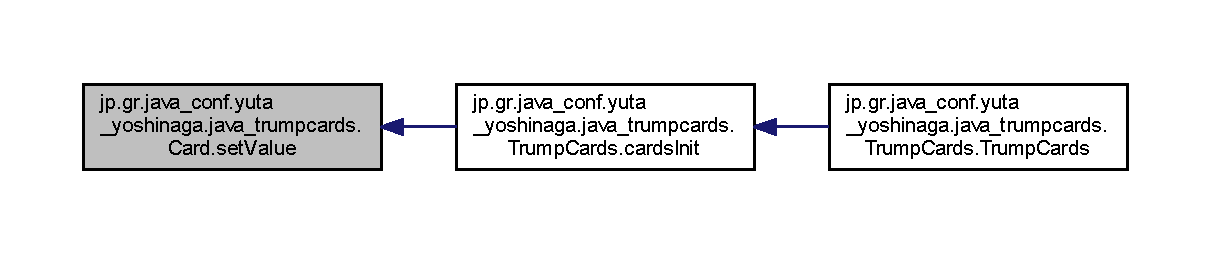
\includegraphics[width=350pt]{classjp_1_1gr_1_1java__conf_1_1yuta__yoshinaga_1_1java__trumpcards_1_1_card_a64976287ff631099e8cde6717b1611c6_icgraph}
\end{center}
\end{figure}


The documentation for this class was generated from the following file\+:\begin{DoxyCompactItemize}
\item 
jp/gr/java\+\_\+conf/yuta\+\_\+yoshinaga/java\+\_\+trumpcards/\hyperlink{_card_8java}{Card.\+java}\end{DoxyCompactItemize}

\hypertarget{classjp_1_1gr_1_1java__conf_1_1yuta__yoshinaga_1_1java__trumpcards_1_1_player}{}\section{jp.\+gr.\+java\+\_\+conf.\+yuta\+\_\+yoshinaga.\+java\+\_\+trumpcards.\+Player Class Reference}
\label{classjp_1_1gr_1_1java__conf_1_1yuta__yoshinaga_1_1java__trumpcards_1_1_player}\index{jp.\+gr.\+java\+\_\+conf.\+yuta\+\_\+yoshinaga.\+java\+\_\+trumpcards.\+Player@{jp.\+gr.\+java\+\_\+conf.\+yuta\+\_\+yoshinaga.\+java\+\_\+trumpcards.\+Player}}


プレイヤークラス  




Collaboration diagram for jp.\+gr.\+java\+\_\+conf.\+yuta\+\_\+yoshinaga.\+java\+\_\+trumpcards.\+Player\+:
\nopagebreak
\begin{figure}[H]
\begin{center}
\leavevmode
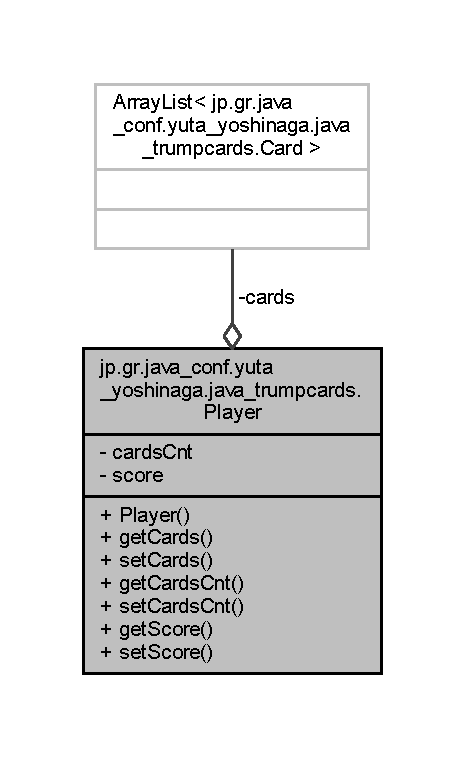
\includegraphics[width=223pt]{classjp_1_1gr_1_1java__conf_1_1yuta__yoshinaga_1_1java__trumpcards_1_1_player__coll__graph}
\end{center}
\end{figure}
\subsection*{Public Member Functions}
\begin{DoxyCompactItemize}
\item 
\hyperlink{classjp_1_1gr_1_1java__conf_1_1yuta__yoshinaga_1_1java__trumpcards_1_1_player_af0a2a1490bdad4fffb17913cf3e2082d}{Player} ()
\begin{DoxyCompactList}\small\item\em コンストラクタ \end{DoxyCompactList}\item 
Array\+List$<$ \hyperlink{classjp_1_1gr_1_1java__conf_1_1yuta__yoshinaga_1_1java__trumpcards_1_1_card}{Card} $>$ \hyperlink{classjp_1_1gr_1_1java__conf_1_1yuta__yoshinaga_1_1java__trumpcards_1_1_player_a6fa54bc94ad8959fbf76abb1107c7385}{get\+Cards} ()
\begin{DoxyCompactList}\small\item\em ゲッター \end{DoxyCompactList}\item 
void \hyperlink{classjp_1_1gr_1_1java__conf_1_1yuta__yoshinaga_1_1java__trumpcards_1_1_player_af3a6a421101b6e8ba60e9578a1b9ec74}{set\+Cards} (Array\+List$<$ \hyperlink{classjp_1_1gr_1_1java__conf_1_1yuta__yoshinaga_1_1java__trumpcards_1_1_card}{Card} $>$ \hyperlink{classjp_1_1gr_1_1java__conf_1_1yuta__yoshinaga_1_1java__trumpcards_1_1_player_a322d1b75dfc3743a73b3327924aad3c2}{cards})
\begin{DoxyCompactList}\small\item\em セッター \end{DoxyCompactList}\item 
int \hyperlink{classjp_1_1gr_1_1java__conf_1_1yuta__yoshinaga_1_1java__trumpcards_1_1_player_ae905e0de5c47509076823375e6995806}{get\+Cards\+Cnt} ()
\begin{DoxyCompactList}\small\item\em ゲッター \end{DoxyCompactList}\item 
void \hyperlink{classjp_1_1gr_1_1java__conf_1_1yuta__yoshinaga_1_1java__trumpcards_1_1_player_a658b393d95e9658b88c8aedcb44a5728}{set\+Cards\+Cnt} (int \hyperlink{classjp_1_1gr_1_1java__conf_1_1yuta__yoshinaga_1_1java__trumpcards_1_1_player_a6f2ad888db0e8899a2f15c8832433f34}{cards\+Cnt})
\begin{DoxyCompactList}\small\item\em セッター \end{DoxyCompactList}\item 
int \hyperlink{classjp_1_1gr_1_1java__conf_1_1yuta__yoshinaga_1_1java__trumpcards_1_1_player_a1158aaad3ebc046ddc15e7f5596b14b4}{get\+Score} ()
\begin{DoxyCompactList}\small\item\em ゲッター \end{DoxyCompactList}\item 
void \hyperlink{classjp_1_1gr_1_1java__conf_1_1yuta__yoshinaga_1_1java__trumpcards_1_1_player_a6c4e87ec9e1c67bfc9b754690b13c542}{set\+Score} (int \hyperlink{classjp_1_1gr_1_1java__conf_1_1yuta__yoshinaga_1_1java__trumpcards_1_1_player_a5eacf559cc78f5ca9ed30e0988810353}{score})
\begin{DoxyCompactList}\small\item\em セッター \end{DoxyCompactList}\end{DoxyCompactItemize}
\subsection*{Private Attributes}
\begin{DoxyCompactItemize}
\item 
\mbox{\Hypertarget{classjp_1_1gr_1_1java__conf_1_1yuta__yoshinaga_1_1java__trumpcards_1_1_player_a322d1b75dfc3743a73b3327924aad3c2}\label{classjp_1_1gr_1_1java__conf_1_1yuta__yoshinaga_1_1java__trumpcards_1_1_player_a322d1b75dfc3743a73b3327924aad3c2}} 
Array\+List$<$ \hyperlink{classjp_1_1gr_1_1java__conf_1_1yuta__yoshinaga_1_1java__trumpcards_1_1_card}{Card} $>$ \hyperlink{classjp_1_1gr_1_1java__conf_1_1yuta__yoshinaga_1_1java__trumpcards_1_1_player_a322d1b75dfc3743a73b3327924aad3c2}{cards}
\begin{DoxyCompactList}\small\item\em プレイヤーカード \end{DoxyCompactList}\item 
\mbox{\Hypertarget{classjp_1_1gr_1_1java__conf_1_1yuta__yoshinaga_1_1java__trumpcards_1_1_player_a6f2ad888db0e8899a2f15c8832433f34}\label{classjp_1_1gr_1_1java__conf_1_1yuta__yoshinaga_1_1java__trumpcards_1_1_player_a6f2ad888db0e8899a2f15c8832433f34}} 
int \hyperlink{classjp_1_1gr_1_1java__conf_1_1yuta__yoshinaga_1_1java__trumpcards_1_1_player_a6f2ad888db0e8899a2f15c8832433f34}{cards\+Cnt}
\begin{DoxyCompactList}\small\item\em プレイヤーカード枚数 \end{DoxyCompactList}\item 
\mbox{\Hypertarget{classjp_1_1gr_1_1java__conf_1_1yuta__yoshinaga_1_1java__trumpcards_1_1_player_a5eacf559cc78f5ca9ed30e0988810353}\label{classjp_1_1gr_1_1java__conf_1_1yuta__yoshinaga_1_1java__trumpcards_1_1_player_a5eacf559cc78f5ca9ed30e0988810353}} 
int \hyperlink{classjp_1_1gr_1_1java__conf_1_1yuta__yoshinaga_1_1java__trumpcards_1_1_player_a5eacf559cc78f5ca9ed30e0988810353}{score}
\begin{DoxyCompactList}\small\item\em プレイヤースコア \end{DoxyCompactList}\end{DoxyCompactItemize}


\subsection{Detailed Description}
プレイヤークラス 

Definition at line 26 of file Player.\+java.



\subsection{Constructor \& Destructor Documentation}
\mbox{\Hypertarget{classjp_1_1gr_1_1java__conf_1_1yuta__yoshinaga_1_1java__trumpcards_1_1_player_af0a2a1490bdad4fffb17913cf3e2082d}\label{classjp_1_1gr_1_1java__conf_1_1yuta__yoshinaga_1_1java__trumpcards_1_1_player_af0a2a1490bdad4fffb17913cf3e2082d}} 
\index{jp\+::gr\+::java\+\_\+conf\+::yuta\+\_\+yoshinaga\+::java\+\_\+trumpcards\+::\+Player@{jp\+::gr\+::java\+\_\+conf\+::yuta\+\_\+yoshinaga\+::java\+\_\+trumpcards\+::\+Player}!Player@{Player}}
\index{Player@{Player}!jp\+::gr\+::java\+\_\+conf\+::yuta\+\_\+yoshinaga\+::java\+\_\+trumpcards\+::\+Player@{jp\+::gr\+::java\+\_\+conf\+::yuta\+\_\+yoshinaga\+::java\+\_\+trumpcards\+::\+Player}}
\subsubsection{\texorpdfstring{Player()}{Player()}}
{\footnotesize\ttfamily public jp.\+gr.\+java\+\_\+conf.\+yuta\+\_\+yoshinaga.\+java\+\_\+trumpcards.\+Player.\+Player (\begin{DoxyParamCaption}{ }\end{DoxyParamCaption})}



コンストラクタ 

\begin{DoxyReturn}{Returns}
ありません 
\end{DoxyReturn}
\begin{DoxyAuthor}{Author}
Yuta Yoshinaga 
\end{DoxyAuthor}
\begin{DoxyDate}{Date}
2019.\+04.\+27 
\end{DoxyDate}


Definition at line 39 of file Player.\+java.



\subsection{Member Function Documentation}
\mbox{\Hypertarget{classjp_1_1gr_1_1java__conf_1_1yuta__yoshinaga_1_1java__trumpcards_1_1_player_a6fa54bc94ad8959fbf76abb1107c7385}\label{classjp_1_1gr_1_1java__conf_1_1yuta__yoshinaga_1_1java__trumpcards_1_1_player_a6fa54bc94ad8959fbf76abb1107c7385}} 
\index{jp\+::gr\+::java\+\_\+conf\+::yuta\+\_\+yoshinaga\+::java\+\_\+trumpcards\+::\+Player@{jp\+::gr\+::java\+\_\+conf\+::yuta\+\_\+yoshinaga\+::java\+\_\+trumpcards\+::\+Player}!get\+Cards@{get\+Cards}}
\index{get\+Cards@{get\+Cards}!jp\+::gr\+::java\+\_\+conf\+::yuta\+\_\+yoshinaga\+::java\+\_\+trumpcards\+::\+Player@{jp\+::gr\+::java\+\_\+conf\+::yuta\+\_\+yoshinaga\+::java\+\_\+trumpcards\+::\+Player}}
\subsubsection{\texorpdfstring{get\+Cards()}{getCards()}}
{\footnotesize\ttfamily Array\+List$<$ \hyperlink{classjp_1_1gr_1_1java__conf_1_1yuta__yoshinaga_1_1java__trumpcards_1_1_card}{Card} $>$ jp.\+gr.\+java\+\_\+conf.\+yuta\+\_\+yoshinaga.\+java\+\_\+trumpcards.\+Player.\+get\+Cards (\begin{DoxyParamCaption}{ }\end{DoxyParamCaption})}



ゲッター 

\begin{DoxyReturn}{Returns}
プレイヤーカード 
\end{DoxyReturn}
\begin{DoxyAuthor}{Author}
Yuta Yoshinaga 
\end{DoxyAuthor}
\begin{DoxyDate}{Date}
2019.\+04.\+27 
\end{DoxyDate}


Definition at line 53 of file Player.\+java.



Referenced by jp.\+gr.\+java\+\_\+conf.\+yuta\+\_\+yoshinaga.\+java\+\_\+trumpcards.\+Black\+Jack.\+dealer\+Hit(), jp.\+gr.\+java\+\_\+conf.\+yuta\+\_\+yoshinaga.\+java\+\_\+trumpcards.\+Black\+Jack.\+game\+Init(), jp.\+gr.\+java\+\_\+conf.\+yuta\+\_\+yoshinaga.\+java\+\_\+trumpcards.\+Black\+Jack.\+game\+Judgment(), jp.\+gr.\+java\+\_\+conf.\+yuta\+\_\+yoshinaga.\+java\+\_\+trumpcards.\+Black\+Jack.\+player\+Hit(), and jp.\+gr.\+java\+\_\+conf.\+yuta\+\_\+yoshinaga.\+java\+\_\+trumpcards.\+Black\+Jack\+Main.\+show\+Status().

Here is the caller graph for this function\+:
\nopagebreak
\begin{figure}[H]
\begin{center}
\leavevmode
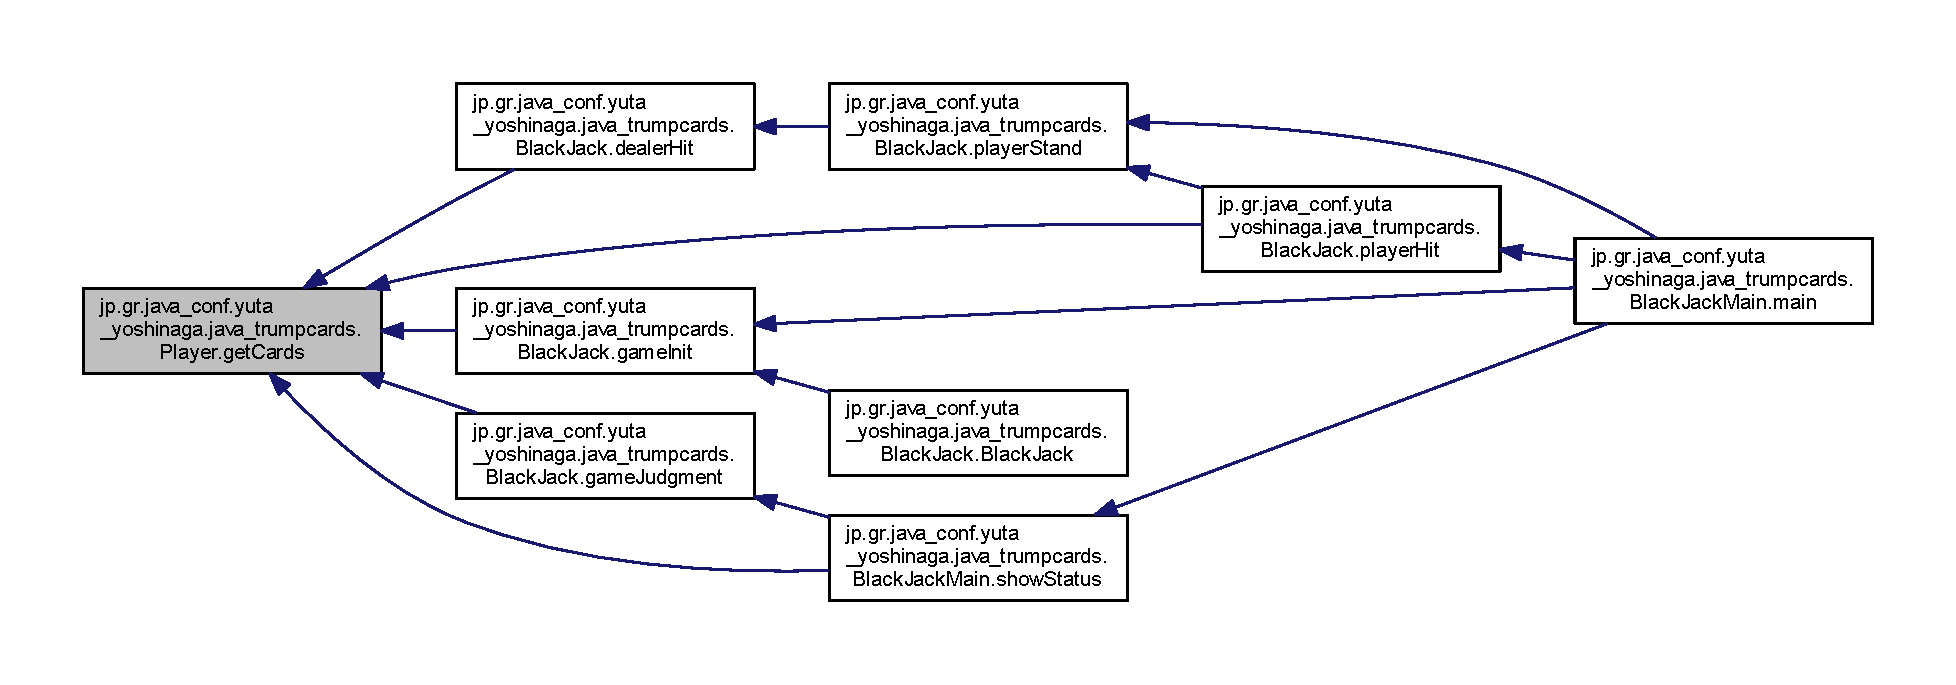
\includegraphics[width=350pt]{classjp_1_1gr_1_1java__conf_1_1yuta__yoshinaga_1_1java__trumpcards_1_1_player_a6fa54bc94ad8959fbf76abb1107c7385_icgraph}
\end{center}
\end{figure}
\mbox{\Hypertarget{classjp_1_1gr_1_1java__conf_1_1yuta__yoshinaga_1_1java__trumpcards_1_1_player_ae905e0de5c47509076823375e6995806}\label{classjp_1_1gr_1_1java__conf_1_1yuta__yoshinaga_1_1java__trumpcards_1_1_player_ae905e0de5c47509076823375e6995806}} 
\index{jp\+::gr\+::java\+\_\+conf\+::yuta\+\_\+yoshinaga\+::java\+\_\+trumpcards\+::\+Player@{jp\+::gr\+::java\+\_\+conf\+::yuta\+\_\+yoshinaga\+::java\+\_\+trumpcards\+::\+Player}!get\+Cards\+Cnt@{get\+Cards\+Cnt}}
\index{get\+Cards\+Cnt@{get\+Cards\+Cnt}!jp\+::gr\+::java\+\_\+conf\+::yuta\+\_\+yoshinaga\+::java\+\_\+trumpcards\+::\+Player@{jp\+::gr\+::java\+\_\+conf\+::yuta\+\_\+yoshinaga\+::java\+\_\+trumpcards\+::\+Player}}
\subsubsection{\texorpdfstring{get\+Cards\+Cnt()}{getCardsCnt()}}
{\footnotesize\ttfamily public int jp.\+gr.\+java\+\_\+conf.\+yuta\+\_\+yoshinaga.\+java\+\_\+trumpcards.\+Player.\+get\+Cards\+Cnt (\begin{DoxyParamCaption}{ }\end{DoxyParamCaption})}



ゲッター 

\begin{DoxyReturn}{Returns}
プレイヤーカード枚数 
\end{DoxyReturn}
\begin{DoxyAuthor}{Author}
Yuta Yoshinaga 
\end{DoxyAuthor}
\begin{DoxyDate}{Date}
2019.\+04.\+27 
\end{DoxyDate}


Definition at line 78 of file Player.\+java.



Referenced by jp.\+gr.\+java\+\_\+conf.\+yuta\+\_\+yoshinaga.\+java\+\_\+trumpcards.\+Black\+Jack.\+dealer\+Hit(), jp.\+gr.\+java\+\_\+conf.\+yuta\+\_\+yoshinaga.\+java\+\_\+trumpcards.\+Black\+Jack.\+game\+Init(), jp.\+gr.\+java\+\_\+conf.\+yuta\+\_\+yoshinaga.\+java\+\_\+trumpcards.\+Black\+Jack.\+game\+Judgment(), jp.\+gr.\+java\+\_\+conf.\+yuta\+\_\+yoshinaga.\+java\+\_\+trumpcards.\+Black\+Jack.\+player\+Hit(), and jp.\+gr.\+java\+\_\+conf.\+yuta\+\_\+yoshinaga.\+java\+\_\+trumpcards.\+Black\+Jack\+Main.\+show\+Status().

Here is the caller graph for this function\+:
\nopagebreak
\begin{figure}[H]
\begin{center}
\leavevmode
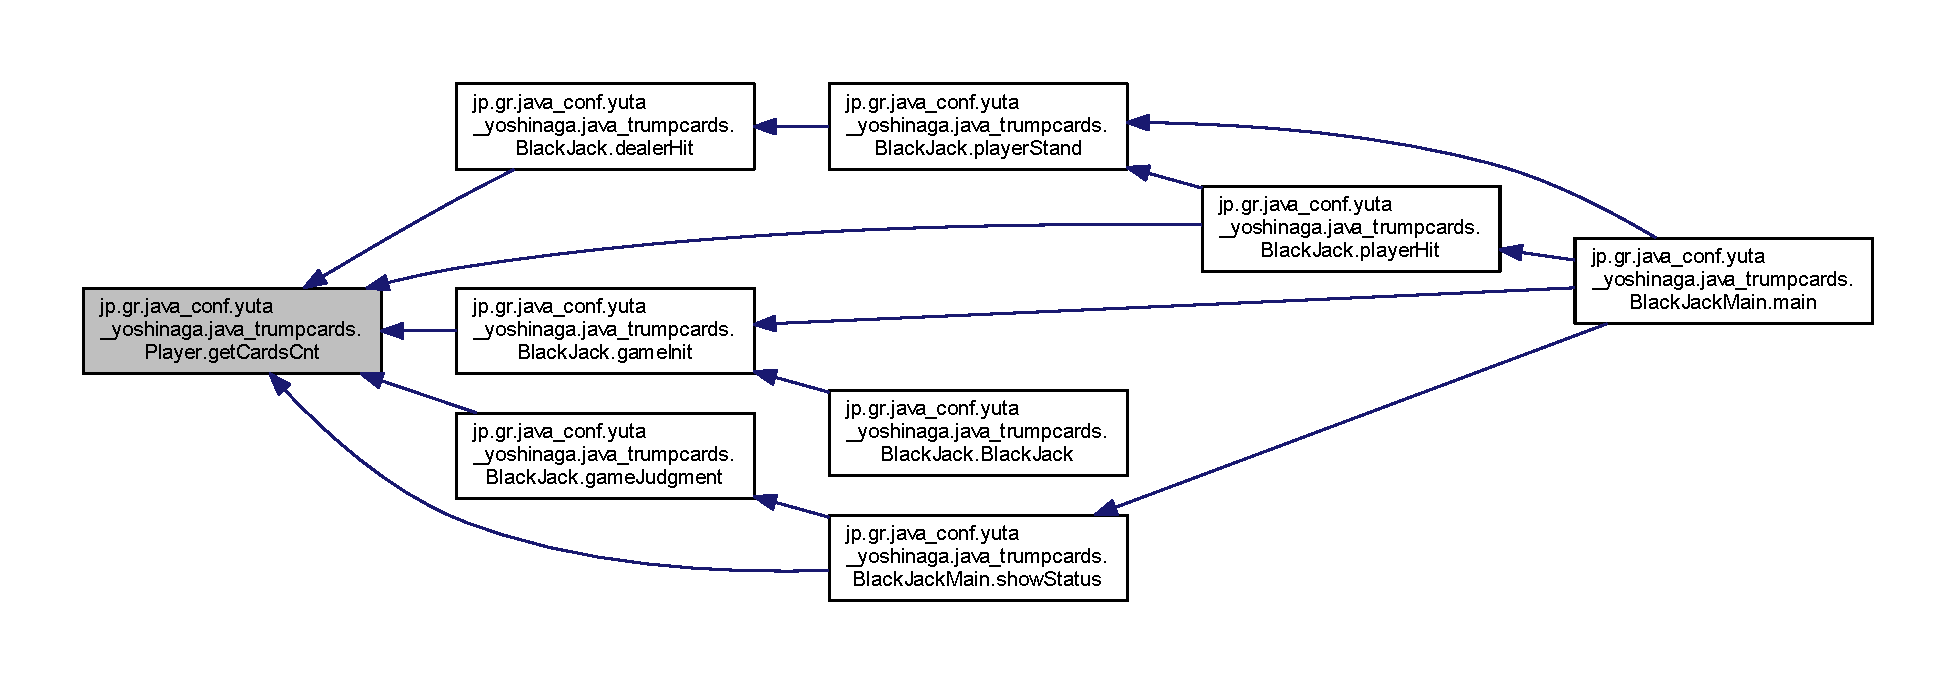
\includegraphics[width=350pt]{classjp_1_1gr_1_1java__conf_1_1yuta__yoshinaga_1_1java__trumpcards_1_1_player_ae905e0de5c47509076823375e6995806_icgraph}
\end{center}
\end{figure}
\mbox{\Hypertarget{classjp_1_1gr_1_1java__conf_1_1yuta__yoshinaga_1_1java__trumpcards_1_1_player_a1158aaad3ebc046ddc15e7f5596b14b4}\label{classjp_1_1gr_1_1java__conf_1_1yuta__yoshinaga_1_1java__trumpcards_1_1_player_a1158aaad3ebc046ddc15e7f5596b14b4}} 
\index{jp\+::gr\+::java\+\_\+conf\+::yuta\+\_\+yoshinaga\+::java\+\_\+trumpcards\+::\+Player@{jp\+::gr\+::java\+\_\+conf\+::yuta\+\_\+yoshinaga\+::java\+\_\+trumpcards\+::\+Player}!get\+Score@{get\+Score}}
\index{get\+Score@{get\+Score}!jp\+::gr\+::java\+\_\+conf\+::yuta\+\_\+yoshinaga\+::java\+\_\+trumpcards\+::\+Player@{jp\+::gr\+::java\+\_\+conf\+::yuta\+\_\+yoshinaga\+::java\+\_\+trumpcards\+::\+Player}}
\subsubsection{\texorpdfstring{get\+Score()}{getScore()}}
{\footnotesize\ttfamily public int jp.\+gr.\+java\+\_\+conf.\+yuta\+\_\+yoshinaga.\+java\+\_\+trumpcards.\+Player.\+get\+Score (\begin{DoxyParamCaption}{ }\end{DoxyParamCaption})}



ゲッター 

\begin{DoxyReturn}{Returns}
プレイヤースコア 
\end{DoxyReturn}
\begin{DoxyAuthor}{Author}
Yuta Yoshinaga 
\end{DoxyAuthor}
\begin{DoxyDate}{Date}
2019.\+04.\+27 
\end{DoxyDate}


Definition at line 103 of file Player.\+java.

\mbox{\Hypertarget{classjp_1_1gr_1_1java__conf_1_1yuta__yoshinaga_1_1java__trumpcards_1_1_player_af3a6a421101b6e8ba60e9578a1b9ec74}\label{classjp_1_1gr_1_1java__conf_1_1yuta__yoshinaga_1_1java__trumpcards_1_1_player_af3a6a421101b6e8ba60e9578a1b9ec74}} 
\index{jp\+::gr\+::java\+\_\+conf\+::yuta\+\_\+yoshinaga\+::java\+\_\+trumpcards\+::\+Player@{jp\+::gr\+::java\+\_\+conf\+::yuta\+\_\+yoshinaga\+::java\+\_\+trumpcards\+::\+Player}!set\+Cards@{set\+Cards}}
\index{set\+Cards@{set\+Cards}!jp\+::gr\+::java\+\_\+conf\+::yuta\+\_\+yoshinaga\+::java\+\_\+trumpcards\+::\+Player@{jp\+::gr\+::java\+\_\+conf\+::yuta\+\_\+yoshinaga\+::java\+\_\+trumpcards\+::\+Player}}
\subsubsection{\texorpdfstring{set\+Cards()}{setCards()}}
{\footnotesize\ttfamily public void jp.\+gr.\+java\+\_\+conf.\+yuta\+\_\+yoshinaga.\+java\+\_\+trumpcards.\+Player.\+set\+Cards (\begin{DoxyParamCaption}\item[{Array\+List$<$ \hyperlink{classjp_1_1gr_1_1java__conf_1_1yuta__yoshinaga_1_1java__trumpcards_1_1_card}{Card} $>$}]{cards }\end{DoxyParamCaption})}



セッター 


\begin{DoxyParams}[1]{Parameters}
\mbox{\tt in}  & {\em Array\+List$<$\+Card$>$} & cards プレイヤーカード \\
\hline
\end{DoxyParams}
\begin{DoxyReturn}{Returns}
ありません 
\end{DoxyReturn}
\begin{DoxyAuthor}{Author}
Yuta Yoshinaga 
\end{DoxyAuthor}
\begin{DoxyDate}{Date}
2019.\+04.\+27 
\end{DoxyDate}


Definition at line 66 of file Player.\+java.



Referenced by jp.\+gr.\+java\+\_\+conf.\+yuta\+\_\+yoshinaga.\+java\+\_\+trumpcards.\+Black\+Jack.\+game\+Init().

Here is the caller graph for this function\+:
\nopagebreak
\begin{figure}[H]
\begin{center}
\leavevmode
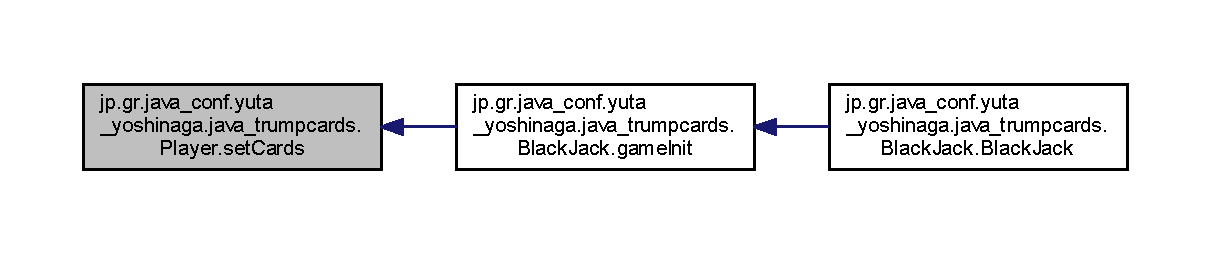
\includegraphics[width=350pt]{classjp_1_1gr_1_1java__conf_1_1yuta__yoshinaga_1_1java__trumpcards_1_1_player_af3a6a421101b6e8ba60e9578a1b9ec74_icgraph}
\end{center}
\end{figure}
\mbox{\Hypertarget{classjp_1_1gr_1_1java__conf_1_1yuta__yoshinaga_1_1java__trumpcards_1_1_player_a658b393d95e9658b88c8aedcb44a5728}\label{classjp_1_1gr_1_1java__conf_1_1yuta__yoshinaga_1_1java__trumpcards_1_1_player_a658b393d95e9658b88c8aedcb44a5728}} 
\index{jp\+::gr\+::java\+\_\+conf\+::yuta\+\_\+yoshinaga\+::java\+\_\+trumpcards\+::\+Player@{jp\+::gr\+::java\+\_\+conf\+::yuta\+\_\+yoshinaga\+::java\+\_\+trumpcards\+::\+Player}!set\+Cards\+Cnt@{set\+Cards\+Cnt}}
\index{set\+Cards\+Cnt@{set\+Cards\+Cnt}!jp\+::gr\+::java\+\_\+conf\+::yuta\+\_\+yoshinaga\+::java\+\_\+trumpcards\+::\+Player@{jp\+::gr\+::java\+\_\+conf\+::yuta\+\_\+yoshinaga\+::java\+\_\+trumpcards\+::\+Player}}
\subsubsection{\texorpdfstring{set\+Cards\+Cnt()}{setCardsCnt()}}
{\footnotesize\ttfamily public void jp.\+gr.\+java\+\_\+conf.\+yuta\+\_\+yoshinaga.\+java\+\_\+trumpcards.\+Player.\+set\+Cards\+Cnt (\begin{DoxyParamCaption}\item[{int}]{cards\+Cnt }\end{DoxyParamCaption})}



セッター 


\begin{DoxyParams}[1]{Parameters}
\mbox{\tt in}  & {\em int} & cards\+Cnt プレイヤーカード枚数 \\
\hline
\end{DoxyParams}
\begin{DoxyReturn}{Returns}
ありません 
\end{DoxyReturn}
\begin{DoxyAuthor}{Author}
Yuta Yoshinaga 
\end{DoxyAuthor}
\begin{DoxyDate}{Date}
2019.\+04.\+27 
\end{DoxyDate}


Definition at line 91 of file Player.\+java.



Referenced by jp.\+gr.\+java\+\_\+conf.\+yuta\+\_\+yoshinaga.\+java\+\_\+trumpcards.\+Black\+Jack.\+dealer\+Hit(), jp.\+gr.\+java\+\_\+conf.\+yuta\+\_\+yoshinaga.\+java\+\_\+trumpcards.\+Black\+Jack.\+game\+Init(), and jp.\+gr.\+java\+\_\+conf.\+yuta\+\_\+yoshinaga.\+java\+\_\+trumpcards.\+Black\+Jack.\+player\+Hit().

Here is the caller graph for this function\+:
\nopagebreak
\begin{figure}[H]
\begin{center}
\leavevmode
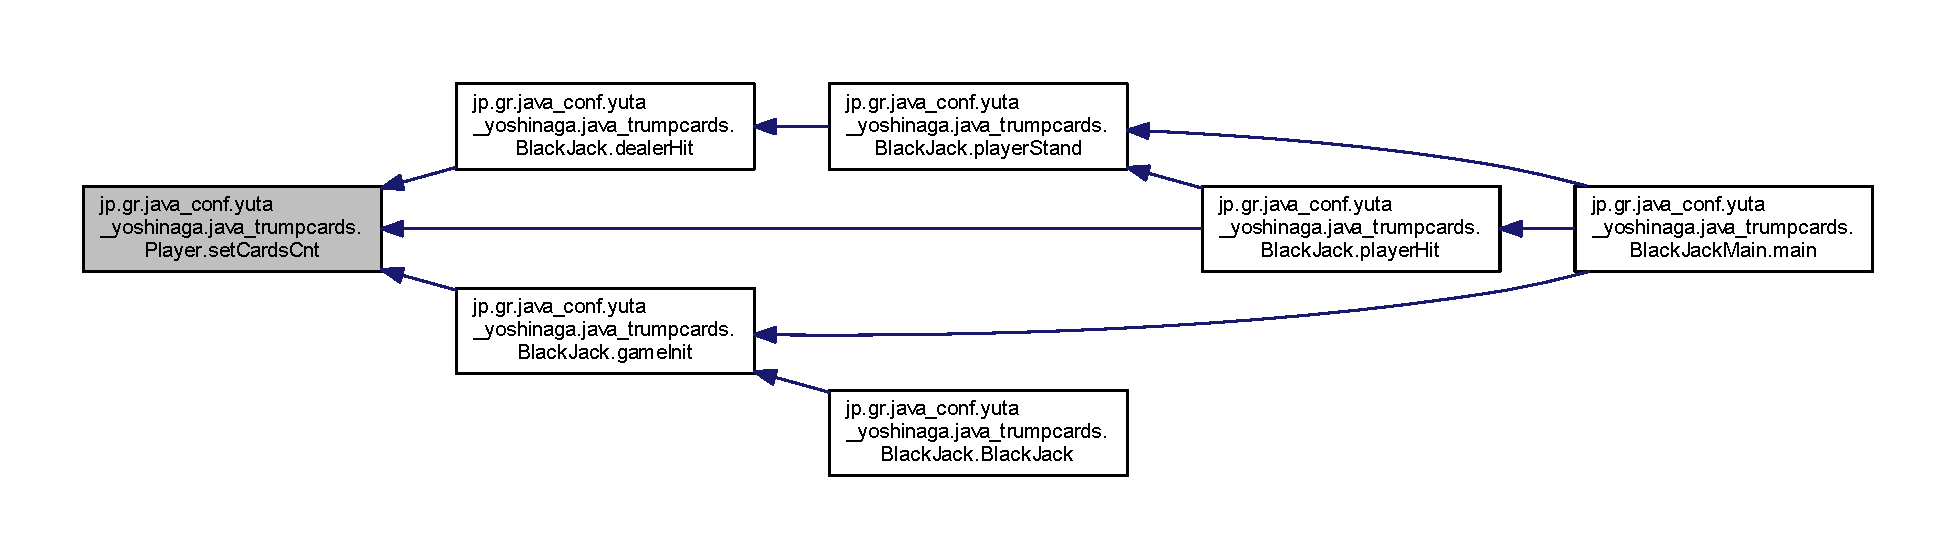
\includegraphics[width=350pt]{classjp_1_1gr_1_1java__conf_1_1yuta__yoshinaga_1_1java__trumpcards_1_1_player_a658b393d95e9658b88c8aedcb44a5728_icgraph}
\end{center}
\end{figure}
\mbox{\Hypertarget{classjp_1_1gr_1_1java__conf_1_1yuta__yoshinaga_1_1java__trumpcards_1_1_player_a6c4e87ec9e1c67bfc9b754690b13c542}\label{classjp_1_1gr_1_1java__conf_1_1yuta__yoshinaga_1_1java__trumpcards_1_1_player_a6c4e87ec9e1c67bfc9b754690b13c542}} 
\index{jp\+::gr\+::java\+\_\+conf\+::yuta\+\_\+yoshinaga\+::java\+\_\+trumpcards\+::\+Player@{jp\+::gr\+::java\+\_\+conf\+::yuta\+\_\+yoshinaga\+::java\+\_\+trumpcards\+::\+Player}!set\+Score@{set\+Score}}
\index{set\+Score@{set\+Score}!jp\+::gr\+::java\+\_\+conf\+::yuta\+\_\+yoshinaga\+::java\+\_\+trumpcards\+::\+Player@{jp\+::gr\+::java\+\_\+conf\+::yuta\+\_\+yoshinaga\+::java\+\_\+trumpcards\+::\+Player}}
\subsubsection{\texorpdfstring{set\+Score()}{setScore()}}
{\footnotesize\ttfamily public void jp.\+gr.\+java\+\_\+conf.\+yuta\+\_\+yoshinaga.\+java\+\_\+trumpcards.\+Player.\+set\+Score (\begin{DoxyParamCaption}\item[{int}]{score }\end{DoxyParamCaption})}



セッター 


\begin{DoxyParams}[1]{Parameters}
\mbox{\tt in}  & {\em int} & score プレイヤースコア \\
\hline
\end{DoxyParams}
\begin{DoxyReturn}{Returns}
ありません 
\end{DoxyReturn}
\begin{DoxyAuthor}{Author}
Yuta Yoshinaga 
\end{DoxyAuthor}
\begin{DoxyDate}{Date}
2019.\+04.\+27 
\end{DoxyDate}


Definition at line 116 of file Player.\+java.



The documentation for this class was generated from the following file\+:\begin{DoxyCompactItemize}
\item 
jp/gr/java\+\_\+conf/yuta\+\_\+yoshinaga/java\+\_\+trumpcards/\hyperlink{_player_8java}{Player.\+java}\end{DoxyCompactItemize}

\hypertarget{classjp_1_1gr_1_1java__conf_1_1yuta__yoshinaga_1_1java__trumpcards_1_1_trump_cards}{}\section{jp.\+gr.\+java\+\_\+conf.\+yuta\+\_\+yoshinaga.\+java\+\_\+trumpcards.\+Trump\+Cards Class Reference}
\label{classjp_1_1gr_1_1java__conf_1_1yuta__yoshinaga_1_1java__trumpcards_1_1_trump_cards}\index{jp.\+gr.\+java\+\_\+conf.\+yuta\+\_\+yoshinaga.\+java\+\_\+trumpcards.\+Trump\+Cards@{jp.\+gr.\+java\+\_\+conf.\+yuta\+\_\+yoshinaga.\+java\+\_\+trumpcards.\+Trump\+Cards}}


トランプカードクラス  




Collaboration diagram for jp.\+gr.\+java\+\_\+conf.\+yuta\+\_\+yoshinaga.\+java\+\_\+trumpcards.\+Trump\+Cards\+:
\nopagebreak
\begin{figure}[H]
\begin{center}
\leavevmode
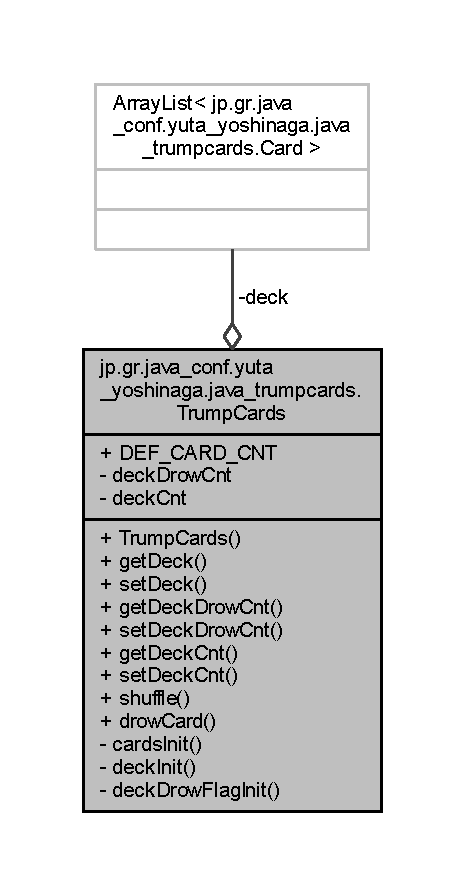
\includegraphics[width=223pt]{classjp_1_1gr_1_1java__conf_1_1yuta__yoshinaga_1_1java__trumpcards_1_1_trump_cards__coll__graph}
\end{center}
\end{figure}
\subsection*{Public Member Functions}
\begin{DoxyCompactItemize}
\item 
\hyperlink{classjp_1_1gr_1_1java__conf_1_1yuta__yoshinaga_1_1java__trumpcards_1_1_trump_cards_aa72c9dd291a7af6a879f7d501debe4cd}{Trump\+Cards} (int joker\+Cnt)
\begin{DoxyCompactList}\small\item\em コンストラクタ \end{DoxyCompactList}\item 
Array\+List$<$ \hyperlink{classjp_1_1gr_1_1java__conf_1_1yuta__yoshinaga_1_1java__trumpcards_1_1_card}{Card} $>$ \hyperlink{classjp_1_1gr_1_1java__conf_1_1yuta__yoshinaga_1_1java__trumpcards_1_1_trump_cards_a45f2e4f7204b7fed4689e9187791df23}{get\+Deck} ()
\begin{DoxyCompactList}\small\item\em ゲッター \end{DoxyCompactList}\item 
void \hyperlink{classjp_1_1gr_1_1java__conf_1_1yuta__yoshinaga_1_1java__trumpcards_1_1_trump_cards_a03b3d1fbcd1d4aaf2ae750ba7c68b9c7}{set\+Deck} (Array\+List$<$ \hyperlink{classjp_1_1gr_1_1java__conf_1_1yuta__yoshinaga_1_1java__trumpcards_1_1_card}{Card} $>$ \hyperlink{classjp_1_1gr_1_1java__conf_1_1yuta__yoshinaga_1_1java__trumpcards_1_1_trump_cards_a313f49864c7810e4fdcd26ecd3e89ec9}{deck})
\begin{DoxyCompactList}\small\item\em セッター \end{DoxyCompactList}\item 
int \hyperlink{classjp_1_1gr_1_1java__conf_1_1yuta__yoshinaga_1_1java__trumpcards_1_1_trump_cards_a3af28b4f707526b638eb976ce8b348e7}{get\+Deck\+Drow\+Cnt} ()
\begin{DoxyCompactList}\small\item\em ゲッター \end{DoxyCompactList}\item 
void \hyperlink{classjp_1_1gr_1_1java__conf_1_1yuta__yoshinaga_1_1java__trumpcards_1_1_trump_cards_afe29b19a537d9a7416dc4c3b289d3b2b}{set\+Deck\+Drow\+Cnt} (int \hyperlink{classjp_1_1gr_1_1java__conf_1_1yuta__yoshinaga_1_1java__trumpcards_1_1_trump_cards_a07cfdc2af869e26718dcdee36c661c38}{deck\+Drow\+Cnt})
\begin{DoxyCompactList}\small\item\em セッター \end{DoxyCompactList}\item 
int \hyperlink{classjp_1_1gr_1_1java__conf_1_1yuta__yoshinaga_1_1java__trumpcards_1_1_trump_cards_a4173ba48c18b6e9737b868c4fef0da47}{get\+Deck\+Cnt} ()
\begin{DoxyCompactList}\small\item\em ゲッター \end{DoxyCompactList}\item 
void \hyperlink{classjp_1_1gr_1_1java__conf_1_1yuta__yoshinaga_1_1java__trumpcards_1_1_trump_cards_ace7ea688cde83158d04d827b51153fdf}{set\+Deck\+Cnt} (int \hyperlink{classjp_1_1gr_1_1java__conf_1_1yuta__yoshinaga_1_1java__trumpcards_1_1_trump_cards_af6c55082de7cb0c1a873e97ce45a8597}{deck\+Cnt})
\begin{DoxyCompactList}\small\item\em セッター \end{DoxyCompactList}\item 
void \hyperlink{classjp_1_1gr_1_1java__conf_1_1yuta__yoshinaga_1_1java__trumpcards_1_1_trump_cards_af1dc4f53d030d1f772c847810e9367fb}{shuffle} ()
\begin{DoxyCompactList}\small\item\em 山札シャッフル \end{DoxyCompactList}\item 
\hyperlink{classjp_1_1gr_1_1java__conf_1_1yuta__yoshinaga_1_1java__trumpcards_1_1_card}{Card} \hyperlink{classjp_1_1gr_1_1java__conf_1_1yuta__yoshinaga_1_1java__trumpcards_1_1_trump_cards_a762812743e7d271596147b7dbcdd4ada}{drow\+Card} ()
\begin{DoxyCompactList}\small\item\em 山札配る \end{DoxyCompactList}\end{DoxyCompactItemize}
\subsection*{Static Public Attributes}
\begin{DoxyCompactItemize}
\item 
\mbox{\Hypertarget{classjp_1_1gr_1_1java__conf_1_1yuta__yoshinaga_1_1java__trumpcards_1_1_trump_cards_afd2b67f2dcb5a18482ad32cc93dd8f6a}\label{classjp_1_1gr_1_1java__conf_1_1yuta__yoshinaga_1_1java__trumpcards_1_1_trump_cards_afd2b67f2dcb5a18482ad32cc93dd8f6a}} 
static final int {\bfseries D\+E\+F\+\_\+\+C\+A\+R\+D\+\_\+\+C\+NT} = (13 $\ast$ 4)
\end{DoxyCompactItemize}
\subsection*{Private Member Functions}
\begin{DoxyCompactItemize}
\item 
void \hyperlink{classjp_1_1gr_1_1java__conf_1_1yuta__yoshinaga_1_1java__trumpcards_1_1_trump_cards_a8e8a4cda3a952cb6a295274765240808}{cards\+Init} ()
\begin{DoxyCompactList}\small\item\em カード初期化 \end{DoxyCompactList}\item 
void \hyperlink{classjp_1_1gr_1_1java__conf_1_1yuta__yoshinaga_1_1java__trumpcards_1_1_trump_cards_af1a1d8299e1e79a272351c9e4b4026fa}{deck\+Init} ()
\begin{DoxyCompactList}\small\item\em 山札初期化 \end{DoxyCompactList}\item 
void \hyperlink{classjp_1_1gr_1_1java__conf_1_1yuta__yoshinaga_1_1java__trumpcards_1_1_trump_cards_aa1db686e11e2c281976505d527eaffbd}{deck\+Drow\+Flag\+Init} ()
\begin{DoxyCompactList}\small\item\em 山札ドローフラグ初期化 \end{DoxyCompactList}\end{DoxyCompactItemize}
\subsection*{Private Attributes}
\begin{DoxyCompactItemize}
\item 
\mbox{\Hypertarget{classjp_1_1gr_1_1java__conf_1_1yuta__yoshinaga_1_1java__trumpcards_1_1_trump_cards_a313f49864c7810e4fdcd26ecd3e89ec9}\label{classjp_1_1gr_1_1java__conf_1_1yuta__yoshinaga_1_1java__trumpcards_1_1_trump_cards_a313f49864c7810e4fdcd26ecd3e89ec9}} 
Array\+List$<$ \hyperlink{classjp_1_1gr_1_1java__conf_1_1yuta__yoshinaga_1_1java__trumpcards_1_1_card}{Card} $>$ \hyperlink{classjp_1_1gr_1_1java__conf_1_1yuta__yoshinaga_1_1java__trumpcards_1_1_trump_cards_a313f49864c7810e4fdcd26ecd3e89ec9}{deck}
\begin{DoxyCompactList}\small\item\em 山札 \end{DoxyCompactList}\item 
\mbox{\Hypertarget{classjp_1_1gr_1_1java__conf_1_1yuta__yoshinaga_1_1java__trumpcards_1_1_trump_cards_a07cfdc2af869e26718dcdee36c661c38}\label{classjp_1_1gr_1_1java__conf_1_1yuta__yoshinaga_1_1java__trumpcards_1_1_trump_cards_a07cfdc2af869e26718dcdee36c661c38}} 
int \hyperlink{classjp_1_1gr_1_1java__conf_1_1yuta__yoshinaga_1_1java__trumpcards_1_1_trump_cards_a07cfdc2af869e26718dcdee36c661c38}{deck\+Drow\+Cnt}
\begin{DoxyCompactList}\small\item\em 山札配った枚数 \end{DoxyCompactList}\item 
\mbox{\Hypertarget{classjp_1_1gr_1_1java__conf_1_1yuta__yoshinaga_1_1java__trumpcards_1_1_trump_cards_af6c55082de7cb0c1a873e97ce45a8597}\label{classjp_1_1gr_1_1java__conf_1_1yuta__yoshinaga_1_1java__trumpcards_1_1_trump_cards_af6c55082de7cb0c1a873e97ce45a8597}} 
int \hyperlink{classjp_1_1gr_1_1java__conf_1_1yuta__yoshinaga_1_1java__trumpcards_1_1_trump_cards_af6c55082de7cb0c1a873e97ce45a8597}{deck\+Cnt}
\begin{DoxyCompactList}\small\item\em 山札枚数 \end{DoxyCompactList}\end{DoxyCompactItemize}


\subsection{Detailed Description}
トランプカードクラス 

Definition at line 27 of file Trump\+Cards.\+java.



\subsection{Constructor \& Destructor Documentation}
\mbox{\Hypertarget{classjp_1_1gr_1_1java__conf_1_1yuta__yoshinaga_1_1java__trumpcards_1_1_trump_cards_aa72c9dd291a7af6a879f7d501debe4cd}\label{classjp_1_1gr_1_1java__conf_1_1yuta__yoshinaga_1_1java__trumpcards_1_1_trump_cards_aa72c9dd291a7af6a879f7d501debe4cd}} 
\index{jp\+::gr\+::java\+\_\+conf\+::yuta\+\_\+yoshinaga\+::java\+\_\+trumpcards\+::\+Trump\+Cards@{jp\+::gr\+::java\+\_\+conf\+::yuta\+\_\+yoshinaga\+::java\+\_\+trumpcards\+::\+Trump\+Cards}!Trump\+Cards@{Trump\+Cards}}
\index{Trump\+Cards@{Trump\+Cards}!jp\+::gr\+::java\+\_\+conf\+::yuta\+\_\+yoshinaga\+::java\+\_\+trumpcards\+::\+Trump\+Cards@{jp\+::gr\+::java\+\_\+conf\+::yuta\+\_\+yoshinaga\+::java\+\_\+trumpcards\+::\+Trump\+Cards}}
\subsubsection{\texorpdfstring{Trump\+Cards()}{TrumpCards()}}
{\footnotesize\ttfamily public jp.\+gr.\+java\+\_\+conf.\+yuta\+\_\+yoshinaga.\+java\+\_\+trumpcards.\+Trump\+Cards.\+Trump\+Cards (\begin{DoxyParamCaption}\item[{int}]{joker\+Cnt }\end{DoxyParamCaption})}



コンストラクタ 


\begin{DoxyParams}[1]{Parameters}
\mbox{\tt in}  & {\em int} & joker\+Cnt ジョーカー枚数 \\
\hline
\end{DoxyParams}
\begin{DoxyReturn}{Returns}
ありません 
\end{DoxyReturn}
\begin{DoxyAuthor}{Author}
Yuta Yoshinaga 
\end{DoxyAuthor}
\begin{DoxyDate}{Date}
2019.\+04.\+27 
\end{DoxyDate}


Definition at line 42 of file Trump\+Cards.\+java.

Here is the call graph for this function\+:
\nopagebreak
\begin{figure}[H]
\begin{center}
\leavevmode
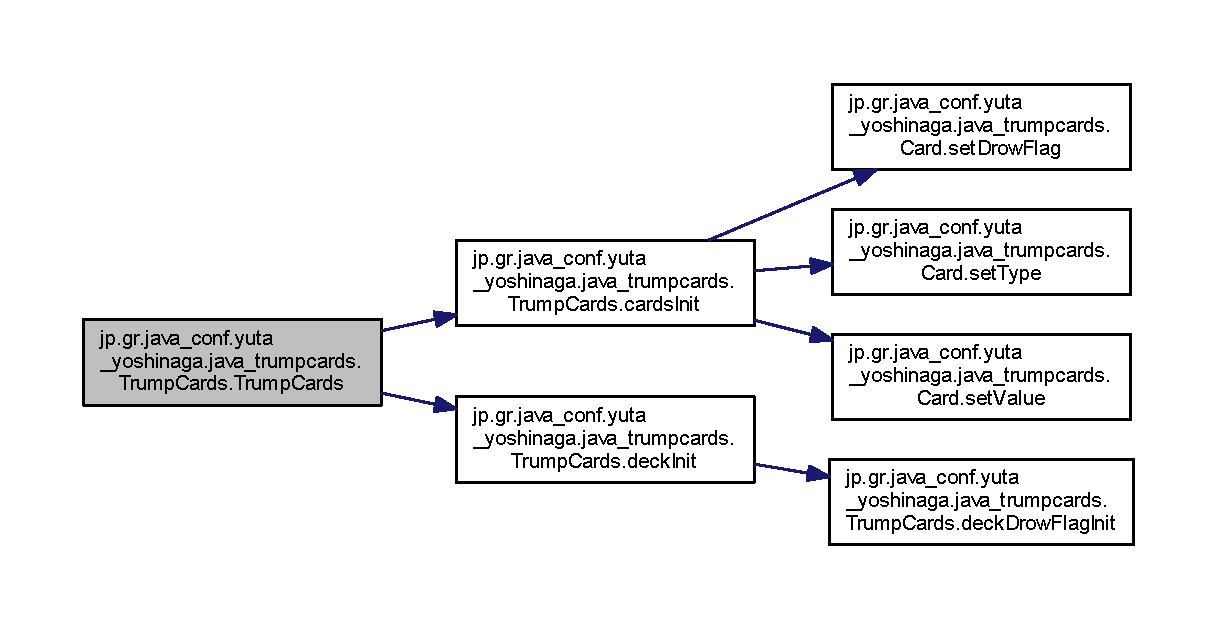
\includegraphics[width=350pt]{classjp_1_1gr_1_1java__conf_1_1yuta__yoshinaga_1_1java__trumpcards_1_1_trump_cards_aa72c9dd291a7af6a879f7d501debe4cd_cgraph}
\end{center}
\end{figure}


\subsection{Member Function Documentation}
\mbox{\Hypertarget{classjp_1_1gr_1_1java__conf_1_1yuta__yoshinaga_1_1java__trumpcards_1_1_trump_cards_a8e8a4cda3a952cb6a295274765240808}\label{classjp_1_1gr_1_1java__conf_1_1yuta__yoshinaga_1_1java__trumpcards_1_1_trump_cards_a8e8a4cda3a952cb6a295274765240808}} 
\index{jp\+::gr\+::java\+\_\+conf\+::yuta\+\_\+yoshinaga\+::java\+\_\+trumpcards\+::\+Trump\+Cards@{jp\+::gr\+::java\+\_\+conf\+::yuta\+\_\+yoshinaga\+::java\+\_\+trumpcards\+::\+Trump\+Cards}!cards\+Init@{cards\+Init}}
\index{cards\+Init@{cards\+Init}!jp\+::gr\+::java\+\_\+conf\+::yuta\+\_\+yoshinaga\+::java\+\_\+trumpcards\+::\+Trump\+Cards@{jp\+::gr\+::java\+\_\+conf\+::yuta\+\_\+yoshinaga\+::java\+\_\+trumpcards\+::\+Trump\+Cards}}
\subsubsection{\texorpdfstring{cards\+Init()}{cardsInit()}}
{\footnotesize\ttfamily private void jp.\+gr.\+java\+\_\+conf.\+yuta\+\_\+yoshinaga.\+java\+\_\+trumpcards.\+Trump\+Cards.\+cards\+Init (\begin{DoxyParamCaption}{ }\end{DoxyParamCaption})\hspace{0.3cm}{\ttfamily [private]}}



カード初期化 

\begin{DoxyReturn}{Returns}
ありません 
\end{DoxyReturn}
\begin{DoxyAuthor}{Author}
Yuta Yoshinaga 
\end{DoxyAuthor}
\begin{DoxyDate}{Date}
2019.\+04.\+27 
\end{DoxyDate}


Definition at line 131 of file Trump\+Cards.\+java.



Referenced by jp.\+gr.\+java\+\_\+conf.\+yuta\+\_\+yoshinaga.\+java\+\_\+trumpcards.\+Trump\+Cards.\+Trump\+Cards().

Here is the call graph for this function\+:
\nopagebreak
\begin{figure}[H]
\begin{center}
\leavevmode
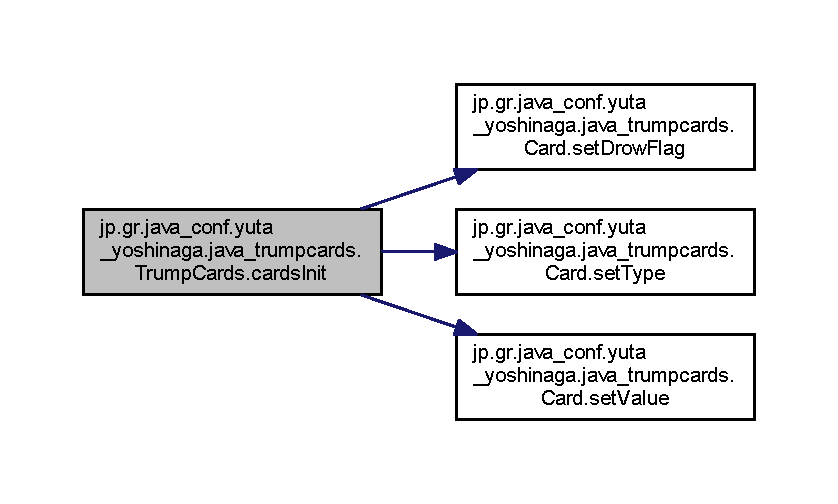
\includegraphics[width=350pt]{classjp_1_1gr_1_1java__conf_1_1yuta__yoshinaga_1_1java__trumpcards_1_1_trump_cards_a8e8a4cda3a952cb6a295274765240808_cgraph}
\end{center}
\end{figure}
Here is the caller graph for this function\+:
\nopagebreak
\begin{figure}[H]
\begin{center}
\leavevmode
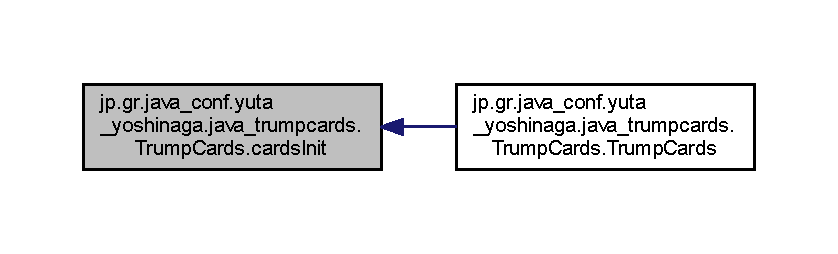
\includegraphics[width=350pt]{classjp_1_1gr_1_1java__conf_1_1yuta__yoshinaga_1_1java__trumpcards_1_1_trump_cards_a8e8a4cda3a952cb6a295274765240808_icgraph}
\end{center}
\end{figure}
\mbox{\Hypertarget{classjp_1_1gr_1_1java__conf_1_1yuta__yoshinaga_1_1java__trumpcards_1_1_trump_cards_aa1db686e11e2c281976505d527eaffbd}\label{classjp_1_1gr_1_1java__conf_1_1yuta__yoshinaga_1_1java__trumpcards_1_1_trump_cards_aa1db686e11e2c281976505d527eaffbd}} 
\index{jp\+::gr\+::java\+\_\+conf\+::yuta\+\_\+yoshinaga\+::java\+\_\+trumpcards\+::\+Trump\+Cards@{jp\+::gr\+::java\+\_\+conf\+::yuta\+\_\+yoshinaga\+::java\+\_\+trumpcards\+::\+Trump\+Cards}!deck\+Drow\+Flag\+Init@{deck\+Drow\+Flag\+Init}}
\index{deck\+Drow\+Flag\+Init@{deck\+Drow\+Flag\+Init}!jp\+::gr\+::java\+\_\+conf\+::yuta\+\_\+yoshinaga\+::java\+\_\+trumpcards\+::\+Trump\+Cards@{jp\+::gr\+::java\+\_\+conf\+::yuta\+\_\+yoshinaga\+::java\+\_\+trumpcards\+::\+Trump\+Cards}}
\subsubsection{\texorpdfstring{deck\+Drow\+Flag\+Init()}{deckDrowFlagInit()}}
{\footnotesize\ttfamily private jp.\+gr.\+java\+\_\+conf.\+yuta\+\_\+yoshinaga.\+java\+\_\+trumpcards.\+Trump\+Cards.\+deck\+Drow\+Flag\+Init (\begin{DoxyParamCaption}{ }\end{DoxyParamCaption})\hspace{0.3cm}{\ttfamily [private]}}



山札ドローフラグ初期化 

\begin{DoxyReturn}{Returns}
ありません 
\end{DoxyReturn}
\begin{DoxyAuthor}{Author}
Yuta Yoshinaga 
\end{DoxyAuthor}
\begin{DoxyDate}{Date}
2019.\+04.\+27 
\end{DoxyDate}


Definition at line 182 of file Trump\+Cards.\+java.



Referenced by jp.\+gr.\+java\+\_\+conf.\+yuta\+\_\+yoshinaga.\+java\+\_\+trumpcards.\+Trump\+Cards.\+deck\+Init(), and jp.\+gr.\+java\+\_\+conf.\+yuta\+\_\+yoshinaga.\+java\+\_\+trumpcards.\+Trump\+Cards.\+shuffle().

Here is the caller graph for this function\+:
\nopagebreak
\begin{figure}[H]
\begin{center}
\leavevmode
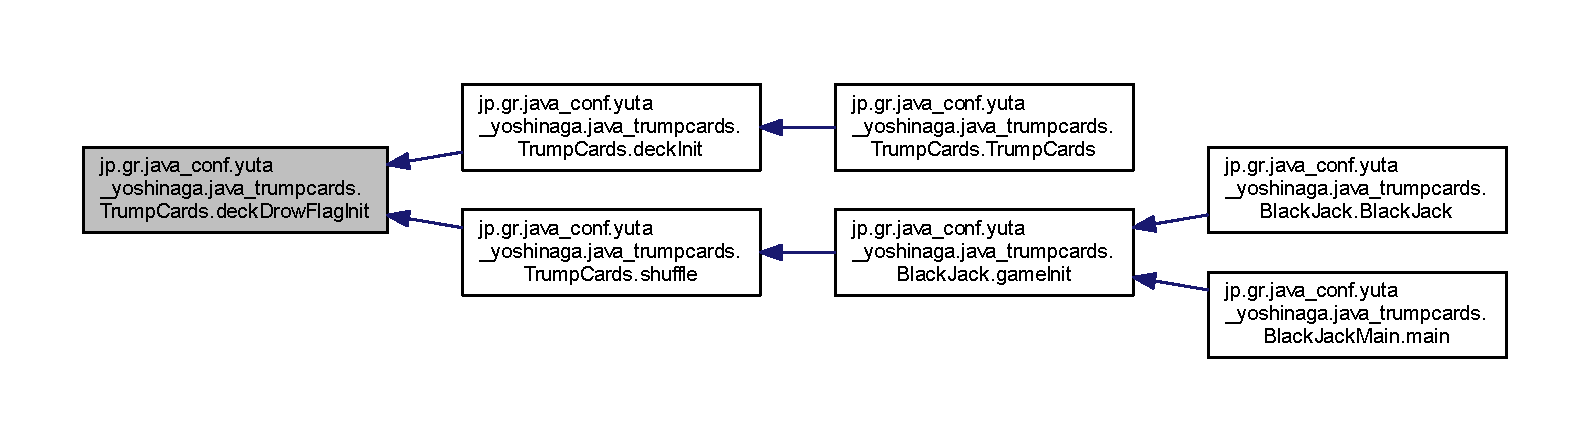
\includegraphics[width=350pt]{classjp_1_1gr_1_1java__conf_1_1yuta__yoshinaga_1_1java__trumpcards_1_1_trump_cards_aa1db686e11e2c281976505d527eaffbd_icgraph}
\end{center}
\end{figure}
\mbox{\Hypertarget{classjp_1_1gr_1_1java__conf_1_1yuta__yoshinaga_1_1java__trumpcards_1_1_trump_cards_af1a1d8299e1e79a272351c9e4b4026fa}\label{classjp_1_1gr_1_1java__conf_1_1yuta__yoshinaga_1_1java__trumpcards_1_1_trump_cards_af1a1d8299e1e79a272351c9e4b4026fa}} 
\index{jp\+::gr\+::java\+\_\+conf\+::yuta\+\_\+yoshinaga\+::java\+\_\+trumpcards\+::\+Trump\+Cards@{jp\+::gr\+::java\+\_\+conf\+::yuta\+\_\+yoshinaga\+::java\+\_\+trumpcards\+::\+Trump\+Cards}!deck\+Init@{deck\+Init}}
\index{deck\+Init@{deck\+Init}!jp\+::gr\+::java\+\_\+conf\+::yuta\+\_\+yoshinaga\+::java\+\_\+trumpcards\+::\+Trump\+Cards@{jp\+::gr\+::java\+\_\+conf\+::yuta\+\_\+yoshinaga\+::java\+\_\+trumpcards\+::\+Trump\+Cards}}
\subsubsection{\texorpdfstring{deck\+Init()}{deckInit()}}
{\footnotesize\ttfamily private void jp.\+gr.\+java\+\_\+conf.\+yuta\+\_\+yoshinaga.\+java\+\_\+trumpcards.\+Trump\+Cards.\+deck\+Init (\begin{DoxyParamCaption}{ }\end{DoxyParamCaption})\hspace{0.3cm}{\ttfamily [private]}}



山札初期化 

\begin{DoxyReturn}{Returns}
ありません 
\end{DoxyReturn}
\begin{DoxyAuthor}{Author}
Yuta Yoshinaga 
\end{DoxyAuthor}
\begin{DoxyDate}{Date}
2019.\+04.\+27 
\end{DoxyDate}


Definition at line 169 of file Trump\+Cards.\+java.



Referenced by jp.\+gr.\+java\+\_\+conf.\+yuta\+\_\+yoshinaga.\+java\+\_\+trumpcards.\+Trump\+Cards.\+Trump\+Cards().

Here is the call graph for this function\+:
\nopagebreak
\begin{figure}[H]
\begin{center}
\leavevmode
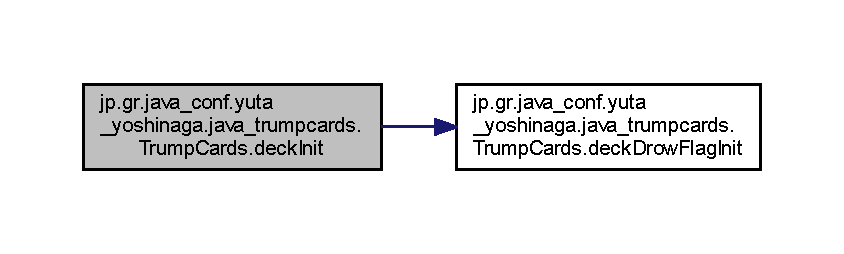
\includegraphics[width=350pt]{classjp_1_1gr_1_1java__conf_1_1yuta__yoshinaga_1_1java__trumpcards_1_1_trump_cards_af1a1d8299e1e79a272351c9e4b4026fa_cgraph}
\end{center}
\end{figure}
Here is the caller graph for this function\+:
\nopagebreak
\begin{figure}[H]
\begin{center}
\leavevmode
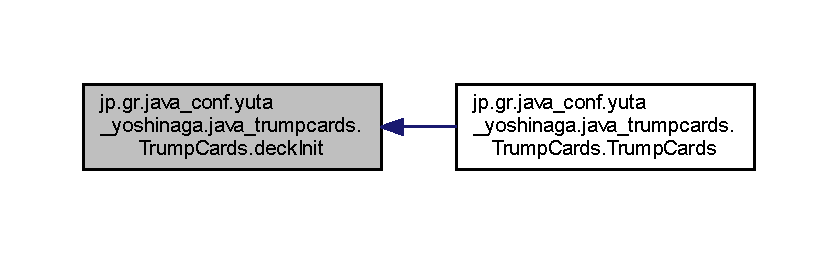
\includegraphics[width=350pt]{classjp_1_1gr_1_1java__conf_1_1yuta__yoshinaga_1_1java__trumpcards_1_1_trump_cards_af1a1d8299e1e79a272351c9e4b4026fa_icgraph}
\end{center}
\end{figure}
\mbox{\Hypertarget{classjp_1_1gr_1_1java__conf_1_1yuta__yoshinaga_1_1java__trumpcards_1_1_trump_cards_a762812743e7d271596147b7dbcdd4ada}\label{classjp_1_1gr_1_1java__conf_1_1yuta__yoshinaga_1_1java__trumpcards_1_1_trump_cards_a762812743e7d271596147b7dbcdd4ada}} 
\index{jp\+::gr\+::java\+\_\+conf\+::yuta\+\_\+yoshinaga\+::java\+\_\+trumpcards\+::\+Trump\+Cards@{jp\+::gr\+::java\+\_\+conf\+::yuta\+\_\+yoshinaga\+::java\+\_\+trumpcards\+::\+Trump\+Cards}!drow\+Card@{drow\+Card}}
\index{drow\+Card@{drow\+Card}!jp\+::gr\+::java\+\_\+conf\+::yuta\+\_\+yoshinaga\+::java\+\_\+trumpcards\+::\+Trump\+Cards@{jp\+::gr\+::java\+\_\+conf\+::yuta\+\_\+yoshinaga\+::java\+\_\+trumpcards\+::\+Trump\+Cards}}
\subsubsection{\texorpdfstring{drow\+Card()}{drowCard()}}
{\footnotesize\ttfamily public jp.\+gr.\+java\+\_\+conf.\+yuta\+\_\+yoshinaga.\+java\+\_\+trumpcards.\+Trump\+Cards.\+drow\+Card (\begin{DoxyParamCaption}{ }\end{DoxyParamCaption})}



山札配る 

\begin{DoxyReturn}{Returns}
カードクラス 
\end{DoxyReturn}
\begin{DoxyAuthor}{Author}
Yuta Yoshinaga 
\end{DoxyAuthor}
\begin{DoxyDate}{Date}
2019.\+04.\+27 
\end{DoxyDate}


Definition at line 210 of file Trump\+Cards.\+java.



Referenced by jp.\+gr.\+java\+\_\+conf.\+yuta\+\_\+yoshinaga.\+java\+\_\+trumpcards.\+Black\+Jack.\+dealer\+Hit(), jp.\+gr.\+java\+\_\+conf.\+yuta\+\_\+yoshinaga.\+java\+\_\+trumpcards.\+Black\+Jack.\+game\+Init(), and jp.\+gr.\+java\+\_\+conf.\+yuta\+\_\+yoshinaga.\+java\+\_\+trumpcards.\+Black\+Jack.\+player\+Hit().

Here is the call graph for this function\+:
\nopagebreak
\begin{figure}[H]
\begin{center}
\leavevmode
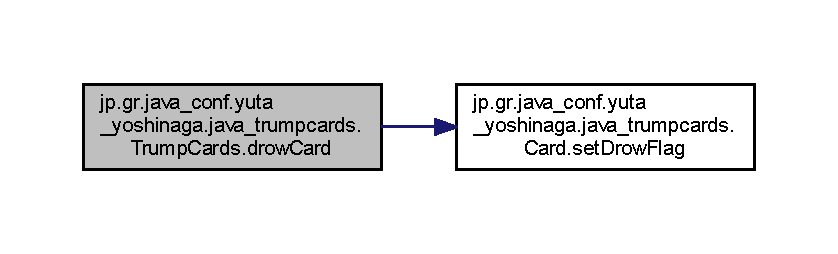
\includegraphics[width=350pt]{classjp_1_1gr_1_1java__conf_1_1yuta__yoshinaga_1_1java__trumpcards_1_1_trump_cards_a762812743e7d271596147b7dbcdd4ada_cgraph}
\end{center}
\end{figure}
Here is the caller graph for this function\+:
\nopagebreak
\begin{figure}[H]
\begin{center}
\leavevmode
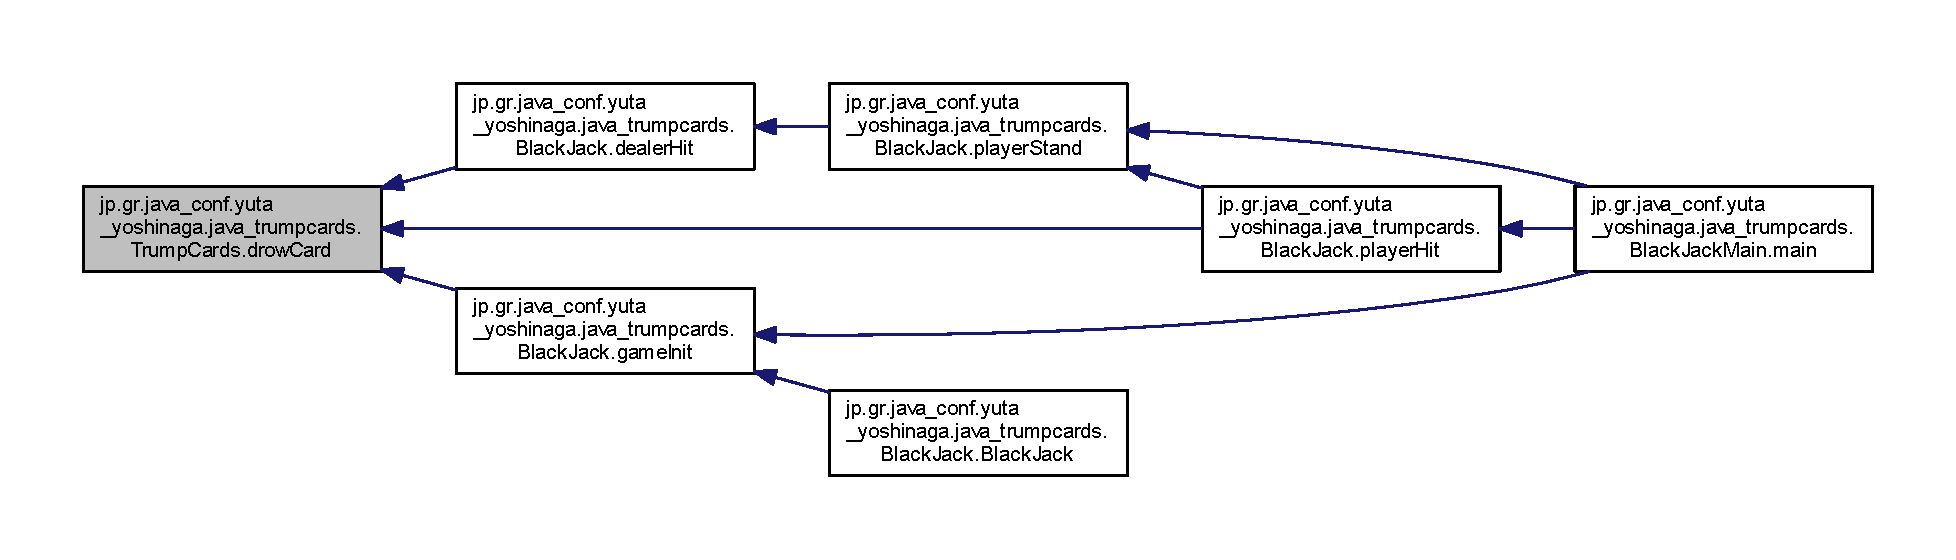
\includegraphics[width=350pt]{classjp_1_1gr_1_1java__conf_1_1yuta__yoshinaga_1_1java__trumpcards_1_1_trump_cards_a762812743e7d271596147b7dbcdd4ada_icgraph}
\end{center}
\end{figure}
\mbox{\Hypertarget{classjp_1_1gr_1_1java__conf_1_1yuta__yoshinaga_1_1java__trumpcards_1_1_trump_cards_a45f2e4f7204b7fed4689e9187791df23}\label{classjp_1_1gr_1_1java__conf_1_1yuta__yoshinaga_1_1java__trumpcards_1_1_trump_cards_a45f2e4f7204b7fed4689e9187791df23}} 
\index{jp\+::gr\+::java\+\_\+conf\+::yuta\+\_\+yoshinaga\+::java\+\_\+trumpcards\+::\+Trump\+Cards@{jp\+::gr\+::java\+\_\+conf\+::yuta\+\_\+yoshinaga\+::java\+\_\+trumpcards\+::\+Trump\+Cards}!get\+Deck@{get\+Deck}}
\index{get\+Deck@{get\+Deck}!jp\+::gr\+::java\+\_\+conf\+::yuta\+\_\+yoshinaga\+::java\+\_\+trumpcards\+::\+Trump\+Cards@{jp\+::gr\+::java\+\_\+conf\+::yuta\+\_\+yoshinaga\+::java\+\_\+trumpcards\+::\+Trump\+Cards}}
\subsubsection{\texorpdfstring{get\+Deck()}{getDeck()}}
{\footnotesize\ttfamily public Array\+List$<$ \hyperlink{classjp_1_1gr_1_1java__conf_1_1yuta__yoshinaga_1_1java__trumpcards_1_1_card}{Card} $>$ jp.\+gr.\+java\+\_\+conf.\+yuta\+\_\+yoshinaga.\+java\+\_\+trumpcards.\+Trump\+Cards.\+get\+Deck (\begin{DoxyParamCaption}{ }\end{DoxyParamCaption})}



ゲッター 

\begin{DoxyReturn}{Returns}
山札 
\end{DoxyReturn}
\begin{DoxyAuthor}{Author}
Yuta Yoshinaga 
\end{DoxyAuthor}
\begin{DoxyDate}{Date}
2019.\+04.\+27 
\end{DoxyDate}


Definition at line 56 of file Trump\+Cards.\+java.

\mbox{\Hypertarget{classjp_1_1gr_1_1java__conf_1_1yuta__yoshinaga_1_1java__trumpcards_1_1_trump_cards_a4173ba48c18b6e9737b868c4fef0da47}\label{classjp_1_1gr_1_1java__conf_1_1yuta__yoshinaga_1_1java__trumpcards_1_1_trump_cards_a4173ba48c18b6e9737b868c4fef0da47}} 
\index{jp\+::gr\+::java\+\_\+conf\+::yuta\+\_\+yoshinaga\+::java\+\_\+trumpcards\+::\+Trump\+Cards@{jp\+::gr\+::java\+\_\+conf\+::yuta\+\_\+yoshinaga\+::java\+\_\+trumpcards\+::\+Trump\+Cards}!get\+Deck\+Cnt@{get\+Deck\+Cnt}}
\index{get\+Deck\+Cnt@{get\+Deck\+Cnt}!jp\+::gr\+::java\+\_\+conf\+::yuta\+\_\+yoshinaga\+::java\+\_\+trumpcards\+::\+Trump\+Cards@{jp\+::gr\+::java\+\_\+conf\+::yuta\+\_\+yoshinaga\+::java\+\_\+trumpcards\+::\+Trump\+Cards}}
\subsubsection{\texorpdfstring{get\+Deck\+Cnt()}{getDeckCnt()}}
{\footnotesize\ttfamily public int jp.\+gr.\+java\+\_\+conf.\+yuta\+\_\+yoshinaga.\+java\+\_\+trumpcards.\+Trump\+Cards.\+get\+Deck\+Cnt (\begin{DoxyParamCaption}{ }\end{DoxyParamCaption})}



ゲッター 

\begin{DoxyReturn}{Returns}
山札枚数 
\end{DoxyReturn}
\begin{DoxyAuthor}{Author}
Yuta Yoshinaga 
\end{DoxyAuthor}
\begin{DoxyDate}{Date}
2019.\+04.\+27 
\end{DoxyDate}


Definition at line 106 of file Trump\+Cards.\+java.

\mbox{\Hypertarget{classjp_1_1gr_1_1java__conf_1_1yuta__yoshinaga_1_1java__trumpcards_1_1_trump_cards_a3af28b4f707526b638eb976ce8b348e7}\label{classjp_1_1gr_1_1java__conf_1_1yuta__yoshinaga_1_1java__trumpcards_1_1_trump_cards_a3af28b4f707526b638eb976ce8b348e7}} 
\index{jp\+::gr\+::java\+\_\+conf\+::yuta\+\_\+yoshinaga\+::java\+\_\+trumpcards\+::\+Trump\+Cards@{jp\+::gr\+::java\+\_\+conf\+::yuta\+\_\+yoshinaga\+::java\+\_\+trumpcards\+::\+Trump\+Cards}!get\+Deck\+Drow\+Cnt@{get\+Deck\+Drow\+Cnt}}
\index{get\+Deck\+Drow\+Cnt@{get\+Deck\+Drow\+Cnt}!jp\+::gr\+::java\+\_\+conf\+::yuta\+\_\+yoshinaga\+::java\+\_\+trumpcards\+::\+Trump\+Cards@{jp\+::gr\+::java\+\_\+conf\+::yuta\+\_\+yoshinaga\+::java\+\_\+trumpcards\+::\+Trump\+Cards}}
\subsubsection{\texorpdfstring{get\+Deck\+Drow\+Cnt()}{getDeckDrowCnt()}}
{\footnotesize\ttfamily public int jp.\+gr.\+java\+\_\+conf.\+yuta\+\_\+yoshinaga.\+java\+\_\+trumpcards.\+Trump\+Cards.\+get\+Deck\+Drow\+Cnt (\begin{DoxyParamCaption}{ }\end{DoxyParamCaption})}



ゲッター 

\begin{DoxyReturn}{Returns}
山札配った枚数 
\end{DoxyReturn}
\begin{DoxyAuthor}{Author}
Yuta Yoshinaga 
\end{DoxyAuthor}
\begin{DoxyDate}{Date}
2019.\+04.\+27 
\end{DoxyDate}


Definition at line 81 of file Trump\+Cards.\+java.

\mbox{\Hypertarget{classjp_1_1gr_1_1java__conf_1_1yuta__yoshinaga_1_1java__trumpcards_1_1_trump_cards_a03b3d1fbcd1d4aaf2ae750ba7c68b9c7}\label{classjp_1_1gr_1_1java__conf_1_1yuta__yoshinaga_1_1java__trumpcards_1_1_trump_cards_a03b3d1fbcd1d4aaf2ae750ba7c68b9c7}} 
\index{jp\+::gr\+::java\+\_\+conf\+::yuta\+\_\+yoshinaga\+::java\+\_\+trumpcards\+::\+Trump\+Cards@{jp\+::gr\+::java\+\_\+conf\+::yuta\+\_\+yoshinaga\+::java\+\_\+trumpcards\+::\+Trump\+Cards}!set\+Deck@{set\+Deck}}
\index{set\+Deck@{set\+Deck}!jp\+::gr\+::java\+\_\+conf\+::yuta\+\_\+yoshinaga\+::java\+\_\+trumpcards\+::\+Trump\+Cards@{jp\+::gr\+::java\+\_\+conf\+::yuta\+\_\+yoshinaga\+::java\+\_\+trumpcards\+::\+Trump\+Cards}}
\subsubsection{\texorpdfstring{set\+Deck()}{setDeck()}}
{\footnotesize\ttfamily public void jp.\+gr.\+java\+\_\+conf.\+yuta\+\_\+yoshinaga.\+java\+\_\+trumpcards.\+Trump\+Cards.\+set\+Deck (\begin{DoxyParamCaption}\item[{Array\+List$<$ \hyperlink{classjp_1_1gr_1_1java__conf_1_1yuta__yoshinaga_1_1java__trumpcards_1_1_card}{Card} $>$}]{deck }\end{DoxyParamCaption})}



セッター 


\begin{DoxyParams}[1]{Parameters}
\mbox{\tt in}  & {\em Array\+List$<$\+Card$>$} & deck 山札 \\
\hline
\end{DoxyParams}
\begin{DoxyReturn}{Returns}
ありません 
\end{DoxyReturn}
\begin{DoxyAuthor}{Author}
Yuta Yoshinaga 
\end{DoxyAuthor}
\begin{DoxyDate}{Date}
2019.\+04.\+27 
\end{DoxyDate}


Definition at line 69 of file Trump\+Cards.\+java.

\mbox{\Hypertarget{classjp_1_1gr_1_1java__conf_1_1yuta__yoshinaga_1_1java__trumpcards_1_1_trump_cards_ace7ea688cde83158d04d827b51153fdf}\label{classjp_1_1gr_1_1java__conf_1_1yuta__yoshinaga_1_1java__trumpcards_1_1_trump_cards_ace7ea688cde83158d04d827b51153fdf}} 
\index{jp\+::gr\+::java\+\_\+conf\+::yuta\+\_\+yoshinaga\+::java\+\_\+trumpcards\+::\+Trump\+Cards@{jp\+::gr\+::java\+\_\+conf\+::yuta\+\_\+yoshinaga\+::java\+\_\+trumpcards\+::\+Trump\+Cards}!set\+Deck\+Cnt@{set\+Deck\+Cnt}}
\index{set\+Deck\+Cnt@{set\+Deck\+Cnt}!jp\+::gr\+::java\+\_\+conf\+::yuta\+\_\+yoshinaga\+::java\+\_\+trumpcards\+::\+Trump\+Cards@{jp\+::gr\+::java\+\_\+conf\+::yuta\+\_\+yoshinaga\+::java\+\_\+trumpcards\+::\+Trump\+Cards}}
\subsubsection{\texorpdfstring{set\+Deck\+Cnt()}{setDeckCnt()}}
{\footnotesize\ttfamily public void jp.\+gr.\+java\+\_\+conf.\+yuta\+\_\+yoshinaga.\+java\+\_\+trumpcards.\+Trump\+Cards.\+set\+Deck\+Cnt (\begin{DoxyParamCaption}\item[{int}]{deck\+Cnt }\end{DoxyParamCaption})}



セッター 


\begin{DoxyParams}[1]{Parameters}
\mbox{\tt in}  & {\em int} & deck\+Cnt 山札枚数 \\
\hline
\end{DoxyParams}
\begin{DoxyReturn}{Returns}
ありません 
\end{DoxyReturn}
\begin{DoxyAuthor}{Author}
Yuta Yoshinaga 
\end{DoxyAuthor}
\begin{DoxyDate}{Date}
2019.\+04.\+27 
\end{DoxyDate}


Definition at line 119 of file Trump\+Cards.\+java.

\mbox{\Hypertarget{classjp_1_1gr_1_1java__conf_1_1yuta__yoshinaga_1_1java__trumpcards_1_1_trump_cards_afe29b19a537d9a7416dc4c3b289d3b2b}\label{classjp_1_1gr_1_1java__conf_1_1yuta__yoshinaga_1_1java__trumpcards_1_1_trump_cards_afe29b19a537d9a7416dc4c3b289d3b2b}} 
\index{jp\+::gr\+::java\+\_\+conf\+::yuta\+\_\+yoshinaga\+::java\+\_\+trumpcards\+::\+Trump\+Cards@{jp\+::gr\+::java\+\_\+conf\+::yuta\+\_\+yoshinaga\+::java\+\_\+trumpcards\+::\+Trump\+Cards}!set\+Deck\+Drow\+Cnt@{set\+Deck\+Drow\+Cnt}}
\index{set\+Deck\+Drow\+Cnt@{set\+Deck\+Drow\+Cnt}!jp\+::gr\+::java\+\_\+conf\+::yuta\+\_\+yoshinaga\+::java\+\_\+trumpcards\+::\+Trump\+Cards@{jp\+::gr\+::java\+\_\+conf\+::yuta\+\_\+yoshinaga\+::java\+\_\+trumpcards\+::\+Trump\+Cards}}
\subsubsection{\texorpdfstring{set\+Deck\+Drow\+Cnt()}{setDeckDrowCnt()}}
{\footnotesize\ttfamily public void jp.\+gr.\+java\+\_\+conf.\+yuta\+\_\+yoshinaga.\+java\+\_\+trumpcards.\+Trump\+Cards.\+set\+Deck\+Drow\+Cnt (\begin{DoxyParamCaption}\item[{int}]{deck\+Drow\+Cnt }\end{DoxyParamCaption})}



セッター 


\begin{DoxyParams}[1]{Parameters}
\mbox{\tt in}  & {\em int} & deck\+Drow\+Cnt 山札配った枚数 \\
\hline
\end{DoxyParams}
\begin{DoxyReturn}{Returns}
ありません 
\end{DoxyReturn}
\begin{DoxyAuthor}{Author}
Yuta Yoshinaga 
\end{DoxyAuthor}
\begin{DoxyDate}{Date}
2019.\+04.\+27 
\end{DoxyDate}


Definition at line 94 of file Trump\+Cards.\+java.

\mbox{\Hypertarget{classjp_1_1gr_1_1java__conf_1_1yuta__yoshinaga_1_1java__trumpcards_1_1_trump_cards_af1dc4f53d030d1f772c847810e9367fb}\label{classjp_1_1gr_1_1java__conf_1_1yuta__yoshinaga_1_1java__trumpcards_1_1_trump_cards_af1dc4f53d030d1f772c847810e9367fb}} 
\index{jp\+::gr\+::java\+\_\+conf\+::yuta\+\_\+yoshinaga\+::java\+\_\+trumpcards\+::\+Trump\+Cards@{jp\+::gr\+::java\+\_\+conf\+::yuta\+\_\+yoshinaga\+::java\+\_\+trumpcards\+::\+Trump\+Cards}!shuffle@{shuffle}}
\index{shuffle@{shuffle}!jp\+::gr\+::java\+\_\+conf\+::yuta\+\_\+yoshinaga\+::java\+\_\+trumpcards\+::\+Trump\+Cards@{jp\+::gr\+::java\+\_\+conf\+::yuta\+\_\+yoshinaga\+::java\+\_\+trumpcards\+::\+Trump\+Cards}}
\subsubsection{\texorpdfstring{shuffle()}{shuffle()}}
{\footnotesize\ttfamily public jp.\+gr.\+java\+\_\+conf.\+yuta\+\_\+yoshinaga.\+java\+\_\+trumpcards.\+Trump\+Cards.\+shuffle (\begin{DoxyParamCaption}{ }\end{DoxyParamCaption})}



山札シャッフル 

\begin{DoxyReturn}{Returns}
ありません 
\end{DoxyReturn}
\begin{DoxyAuthor}{Author}
Yuta Yoshinaga 
\end{DoxyAuthor}
\begin{DoxyDate}{Date}
2019.\+04.\+27 
\end{DoxyDate}


Definition at line 196 of file Trump\+Cards.\+java.



Referenced by jp.\+gr.\+java\+\_\+conf.\+yuta\+\_\+yoshinaga.\+java\+\_\+trumpcards.\+Black\+Jack.\+game\+Init().

Here is the call graph for this function\+:
\nopagebreak
\begin{figure}[H]
\begin{center}
\leavevmode
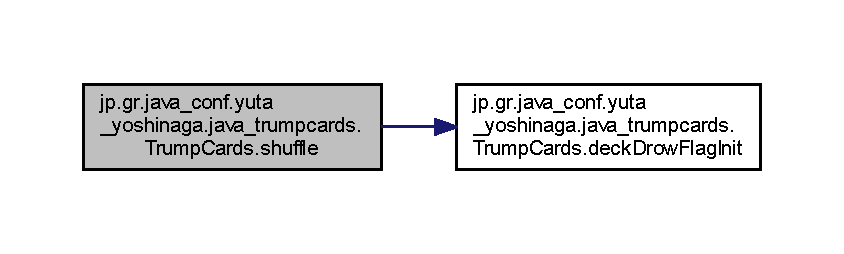
\includegraphics[width=350pt]{classjp_1_1gr_1_1java__conf_1_1yuta__yoshinaga_1_1java__trumpcards_1_1_trump_cards_af1dc4f53d030d1f772c847810e9367fb_cgraph}
\end{center}
\end{figure}
Here is the caller graph for this function\+:
\nopagebreak
\begin{figure}[H]
\begin{center}
\leavevmode
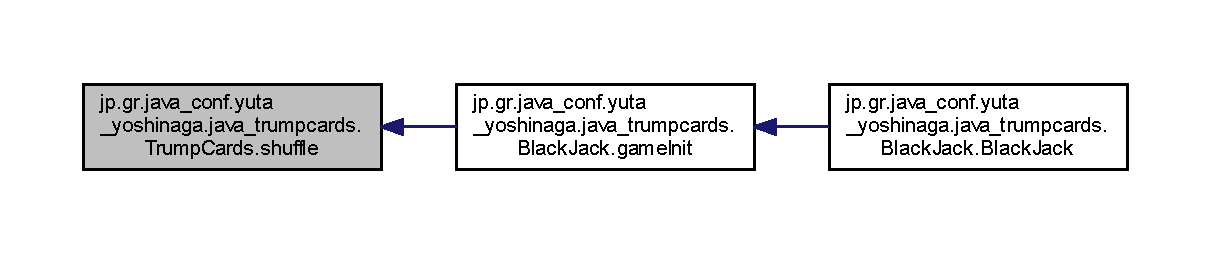
\includegraphics[width=350pt]{classjp_1_1gr_1_1java__conf_1_1yuta__yoshinaga_1_1java__trumpcards_1_1_trump_cards_af1dc4f53d030d1f772c847810e9367fb_icgraph}
\end{center}
\end{figure}


The documentation for this class was generated from the following file\+:\begin{DoxyCompactItemize}
\item 
jp/gr/java\+\_\+conf/yuta\+\_\+yoshinaga/java\+\_\+trumpcards/\hyperlink{_trump_cards_8java}{Trump\+Cards.\+java}\end{DoxyCompactItemize}

\chapter{File Documentation}
\hypertarget{_black_jack_8java}{}\section{jp/gr/java\+\_\+conf/yuta\+\_\+yoshinaga/java\+\_\+trumpcards/\+Black\+Jack.java File Reference}
\label{_black_jack_8java}\index{jp/gr/java\+\_\+conf/yuta\+\_\+yoshinaga/java\+\_\+trumpcards/\+Black\+Jack.\+java@{jp/gr/java\+\_\+conf/yuta\+\_\+yoshinaga/java\+\_\+trumpcards/\+Black\+Jack.\+java}}


ブラックジャッククラス  


\subsection*{Classes}
\begin{DoxyCompactItemize}
\item 
class \hyperlink{classjp_1_1gr_1_1java__conf_1_1yuta__yoshinaga_1_1java__trumpcards_1_1_black_jack}{jp.\+gr.\+java\+\_\+conf.\+yuta\+\_\+yoshinaga.\+java\+\_\+trumpcards.\+Black\+Jack}
\begin{DoxyCompactList}\small\item\em ブラックジャッククラス \end{DoxyCompactList}\end{DoxyCompactItemize}


\subsection{Detailed Description}
ブラックジャッククラス 

\begin{DoxyAuthor}{Author}
Yuta Yoshinaga 
\end{DoxyAuthor}
\begin{DoxyDate}{Date}
2019.\+04.\+27 
\end{DoxyDate}
\begin{DoxyParagraph}{Version}

\end{DoxyParagraph}
\begin{DoxyParagraph}{Revision}

\end{DoxyParagraph}


(c) 2019 Yuta Yoshinaga.


\begin{DoxyItemize}
\item 本ソフトウェアの一部又は全てを無断で複写複製(コピー)することは、 著作権侵害にあたりますので、これを禁止します。
\item 本製品の使用に起因する侵害または特許権その他権利の侵害に関しては 当方は一切その責任を負いません。 
\end{DoxyItemize}
\hypertarget{_card_8java}{}\section{jp/gr/java\+\_\+conf/yuta\+\_\+yoshinaga/java\+\_\+trumpcards/\+Card.java File Reference}
\label{_card_8java}\index{jp/gr/java\+\_\+conf/yuta\+\_\+yoshinaga/java\+\_\+trumpcards/\+Card.\+java@{jp/gr/java\+\_\+conf/yuta\+\_\+yoshinaga/java\+\_\+trumpcards/\+Card.\+java}}


カードクラス  


\subsection*{Classes}
\begin{DoxyCompactItemize}
\item 
class \hyperlink{classjp_1_1gr_1_1java__conf_1_1yuta__yoshinaga_1_1java__trumpcards_1_1_card}{jp.\+gr.\+java\+\_\+conf.\+yuta\+\_\+yoshinaga.\+java\+\_\+trumpcards.\+Card}
\begin{DoxyCompactList}\small\item\em カードクラス \end{DoxyCompactList}\end{DoxyCompactItemize}


\subsection{Detailed Description}
カードクラス 

\begin{DoxyAuthor}{Author}
Yuta Yoshinaga 
\end{DoxyAuthor}
\begin{DoxyDate}{Date}
2019.\+04.\+27 
\end{DoxyDate}
\begin{DoxyParagraph}{Version}

\end{DoxyParagraph}
\begin{DoxyParagraph}{Revision}

\end{DoxyParagraph}


(c) 2019 Yuta Yoshinaga.


\begin{DoxyItemize}
\item 本ソフトウェアの一部又は全てを無断で複写複製(コピー)することは、 著作権侵害にあたりますので、これを禁止します。
\item 本製品の使用に起因する侵害または特許権その他権利の侵害に関しては 当方は一切その責任を負いません。 
\end{DoxyItemize}
\hypertarget{_player_8java}{}\section{jp/gr/java\+\_\+conf/yuta\+\_\+yoshinaga/java\+\_\+trumpcards/\+Player.java File Reference}
\label{_player_8java}\index{jp/gr/java\+\_\+conf/yuta\+\_\+yoshinaga/java\+\_\+trumpcards/\+Player.\+java@{jp/gr/java\+\_\+conf/yuta\+\_\+yoshinaga/java\+\_\+trumpcards/\+Player.\+java}}


プレイヤークラス  


\subsection*{Classes}
\begin{DoxyCompactItemize}
\item 
class \hyperlink{classjp_1_1gr_1_1java__conf_1_1yuta__yoshinaga_1_1java__trumpcards_1_1_player}{jp.\+gr.\+java\+\_\+conf.\+yuta\+\_\+yoshinaga.\+java\+\_\+trumpcards.\+Player}
\begin{DoxyCompactList}\small\item\em プレイヤークラス \end{DoxyCompactList}\end{DoxyCompactItemize}


\subsection{Detailed Description}
プレイヤークラス 

\begin{DoxyAuthor}{Author}
Yuta Yoshinaga 
\end{DoxyAuthor}
\begin{DoxyDate}{Date}
2019.\+04.\+27 
\end{DoxyDate}
\begin{DoxyParagraph}{Version}

\end{DoxyParagraph}
\begin{DoxyParagraph}{Revision}

\end{DoxyParagraph}


(c) 2019 Yuta Yoshinaga.


\begin{DoxyItemize}
\item 本ソフトウェアの一部又は全てを無断で複写複製(コピー)することは、 著作権侵害にあたりますので、これを禁止します。
\item 本製品の使用に起因する侵害または特許権その他権利の侵害に関しては 当方は一切その責任を負いません。 
\end{DoxyItemize}
\hypertarget{_trump_cards_8java}{}\section{jp/gr/java\+\_\+conf/yuta\+\_\+yoshinaga/java\+\_\+trumpcards/\+Trump\+Cards.java File Reference}
\label{_trump_cards_8java}\index{jp/gr/java\+\_\+conf/yuta\+\_\+yoshinaga/java\+\_\+trumpcards/\+Trump\+Cards.\+java@{jp/gr/java\+\_\+conf/yuta\+\_\+yoshinaga/java\+\_\+trumpcards/\+Trump\+Cards.\+java}}


トランプカードクラス  


\subsection*{Classes}
\begin{DoxyCompactItemize}
\item 
class \hyperlink{classjp_1_1gr_1_1java__conf_1_1yuta__yoshinaga_1_1java__trumpcards_1_1_trump_cards}{jp.\+gr.\+java\+\_\+conf.\+yuta\+\_\+yoshinaga.\+java\+\_\+trumpcards.\+Trump\+Cards}
\begin{DoxyCompactList}\small\item\em トランプカードクラス \end{DoxyCompactList}\end{DoxyCompactItemize}


\subsection{Detailed Description}
トランプカードクラス 

\begin{DoxyAuthor}{Author}
Yuta Yoshinaga 
\end{DoxyAuthor}
\begin{DoxyDate}{Date}
2019.\+04.\+27 
\end{DoxyDate}
\begin{DoxyParagraph}{Version}

\end{DoxyParagraph}
\begin{DoxyParagraph}{Revision}

\end{DoxyParagraph}


(c) 2019 Yuta Yoshinaga.


\begin{DoxyItemize}
\item 本ソフトウェアの一部又は全てを無断で複写複製(コピー)することは、 著作権侵害にあたりますので、これを禁止します。
\item 本製品の使用に起因する侵害または特許権その他権利の侵害に関しては 当方は一切その責任を負いません。 
\end{DoxyItemize}
%--- End generated contents ---

% Index
\backmatter
\newpage
\phantomsection
\clearemptydoublepage
\addcontentsline{toc}{chapter}{Index}
\printindex

\end{document}
